%% GENERATED by generate_papers.py -- edit the bank_*.py files, not this file.
\documentclass[11pt,a4paper]{article}
\usepackage[a4paper, top=20mm, bottom=20mm, left=18mm, right=18mm, headheight=14pt]{geometry}
\usepackage[T1]{fontenc}
\usepackage{lmodern}
\usepackage{amsmath, amssymb, mathtools}
\usepackage{braket}
\usepackage{array, tabularx, booktabs, multicol}
\usepackage{enumitem}
\usepackage[dvipsnames]{xcolor}
\usepackage[most]{tcolorbox}
\usepackage{needspace}
\usepackage{fancyhdr, lastpage}
\usepackage{pifont}
\usepackage{tikz}
\usepackage[hidelinks]{hyperref}
\newcolumntype{L}{>{\raggedright\arraybackslash}X}
\definecolor{brand}{HTML}{1F4E79}
\definecolor{okgreen}{HTML}{1B7F3B}
\setlength{\parindent}{0pt}
\setlength{\parskip}{3pt}
\newcommand{\optlabel}[1]{\textbf{(#1)}}
\newcommand{\correctlabel}[1]{\textcolor{okgreen}{\textbf{(#1)}\,\ding{51}}}
\newenvironment{qitem}[1]{\begin{list}{}{\setlength{\leftmargin}{3.3em}\setlength{\labelwidth}{3.1em}%
  \setlength{\labelsep}{0.2em}\setlength{\topsep}{3pt}\setlength{\parsep}{3pt}}\item[\textbf{Q.#1}\hfill]}{\end{list}}
\newcommand{\qsep}{\par\vspace{2pt}{\color{black!15}\hrule}\vspace{4pt}}
\newcommand{\qmeta}[2]{{\footnotesize\color{black!60}\textsc{#1} \;$\cdot$\; #2}\par}
\newtcolorbox{passagebox}[1]{enhanced, breakable, colback=brand!4, colframe=brand!70, fonttitle=\bfseries,
  title={#1}, left=6pt, right=6pt, top=4pt, bottom=4pt}
\newtcolorbox{sectionbanner}{enhanced, colback=brand, colframe=brand, coltext=white, fontupper=\large\bfseries,
  left=8pt, right=8pt, top=6pt, bottom=6pt, sharp corners}
\newtcolorbox{infobox}[1]{enhanced, breakable, colback=black!3, colframe=black!45, fonttitle=\bfseries,
  title={#1}, left=6pt, right=6pt, top=4pt, bottom=4pt}
\newtcolorbox{solbox}[1]{enhanced, breakable, colback=okgreen!3, colframe=okgreen!60!black, fonttitle=\bfseries,
  title={Answer: (#1) \quad Detailed solution}, left=6pt, right=6pt, top=3pt, bottom=4pt, before skip=4pt, after skip=6pt}
\newcommand{\bub}[1]{\tikz[baseline=-0.65ex]\node[draw, circle, inner sep=0pt, minimum size=4.6mm, font=\scriptsize]{#1};}
\allowdisplaybreaks

\begin{document}
\pagestyle{fancy}\fancyhf{}
\fancyhead[L]{\small\color{black!70}Quantum Machine Learning --- Assessment}
\fancyhead[R]{\small\color{black!70}\textbf{Answer Book}}
\fancyfoot[C]{\small Page \thepage\ of \pageref*{LastPage}}
\renewcommand{\headrulewidth}{0.4pt}

\thispagestyle{empty}
\begin{center}
{\color{brand}\rule{\linewidth}{1.2pt}}\\[6pt]
{\Huge\bfseries\color{brand} Quantum Machine Learning}\\[4pt]
{\Large Assessment of QML: encodings, kernels, variational models and the QCNN}\\[4pt]
{\large\bfseries ANSWER BOOK}\\[2pt]
{\color{brand}\rule{\linewidth}{1.2pt}}
\end{center}
This book accompanies the separate \emph{Question Paper} (80 questions, 3 hours, 240 marks). It contains
\begin{enumerate}[leftmargin=1.4em, itemsep=0pt, topsep=2pt]
\item the \textbf{answer key}, section by section, with the topic tested by every question (page~\pageref{key}),
\item a \textbf{topic-wise map} grouping the questions by theme and a \textbf{quick-marking grid} (page~\pageref{topicmap}), and
\item the \textbf{Answer Bank}: every question restated with the correct option marked \textcolor{okgreen}{\ding{51}} and a
      complete solution with derivations (from page~\pageref{bank}).
\end{enumerate}
\begin{infobox}{Marking scheme (every question)}
Each question has \textbf{four} options (A), (B), (C) and (D). \textbf{ONLY ONE} of these four options is correct.\\[2pt]
\begin{tabular}{@{}ll@{}}
\emph{Full marks}: & $+3$ if ONLY the correct option is chosen;\\
\emph{Zero marks}: & $\phantom{+}0$ if none of the options is chosen (question unanswered);\\
\emph{Negative marks}: & $-1$ in all other cases (wrong option, or more than one option chosen).
\end{tabular}
\end{infobox}

\begin{infobox}{How to evaluate}
For each section count $N_{\mathrm c}$ = number of correct answers and $N_{\mathrm w}$ = number of questions answered wrongly (or with more than
one bubble darkened). Section marks $= 3N_{\mathrm c} - N_{\mathrm w}$; unanswered questions score $0$. The total is out of $240$.
Every numerical answer was re-computed independently (NumPy, exact rational arithmetic where possible, an independent NumPy state-vector simulator, and CUDA-Q for the circuits and for the QCNN kernel of \texttt{QML.ipynb}) by
\texttt{verify\_answers.py} in the source folder.
\end{infobox}
\begin{infobox}{Conventions (identical to the Question Paper)}
\footnotesize
\begin{itemize}[leftmargin=1.2em, itemsep=1pt, topsep=2pt]
\item Qubits are numbered $0, 1, \dots$; a basis state $\ket{q_0q_1\dots}$ lists \textbf{qubit 0 first} (as in CUDA-Q's bitstrings), and
      two-qubit matrices use the basis order $\ket{00}, \ket{01}, \ket{10}, \ket{11}$.
\item Gates: $H = \frac{1}{\sqrt2}\begin{psmallmatrix}1&1\\1&-1\end{psmallmatrix}$; $X, Y, Z$ are the Pauli matrices; $S = \operatorname{diag}(1, i)$;
      $R_P(\theta) = e^{-i\theta P/2}$ for $P \in \{X, Y, Z\}$, so $R_Y(\theta)\ket0 = \cos\frac\theta2\ket0 + \sin\frac\theta2\ket1$; CNOT (control $c$,
      target $t$) flips $t$ when $c$ is 1; a controlled-$U$ applies $U$ to the target when the control is $\ket1$.
\item Measurements are in the computational basis; $\langle M\rangle = \braket{\psi|M|\psi}$, so $\langle Z\rangle = P(0) - P(1)$; the Bloch vector is
      $(\langle X\rangle, \langle Y\rangle, \langle Z\rangle)$. Two-term parameter-shift rule: $f'(\theta) = \frac12\big[f(\theta + \frac\pi2) - f(\theta - \frac\pi2)\big]$.
\item Machine learning: labels $y \in \{+1, -1\}$ with prediction $\operatorname{sign}f$ unless stated ($y \in \{0, 1\}$ for cross-entropy);
      MSE $\mathcal L = \frac1M\sum_m(f_m - y_m)^2$; $\sigma(z) = 1/(1 + e^{-z})$; precision $= \frac{TP}{TP + FP}$, recall $= \frac{TP}{TP + FN}$,
      $F_1 = \frac{2PR}{P + R}$; $\ln$ is the natural logarithm. Numerical answers are rounded.
\item \textbf{Notebook} (\texttt{QML.ipynb}, defaults): $2\times4$ images with one line of 2 lit pixels (horizontal $= +1$, vertical $= -1$), background
      noise in $[0, 0.25]$, 20 training / 20 test images, \texttt{SEED = 42}; one qubit per pixel; encoding $R_Y(\pi x_i)$. QCNN
      layer $\ell = 1, 2, \dots$ has 4 shared parameters $\theta_{\ell,1..4}$ = \texttt{theta[4($\ell$-1)]}\,\dots\,\texttt{theta[4($\ell$-1)+3]}:
      convolution block $= \mathrm{CNOT}_{a\to b}\big(R_Y(\theta_{\ell,1})_a\otimes R_Y(\theta_{\ell,2})_b\big)$ on pairs $(0,1), (2,3), \dots$ then $(1,2), (3,4), \dots$;
      pooling block (source $a$, sink $b$) $= \ket1\!\bra1_a\otimes R_Z(\theta_{\ell,3}) + \ket0\!\bra0_a\otimes R_X(\theta_{\ell,4})$, then $a$ is discarded.
      Readout $\langle Z_{\text{out}}\rangle$ with \texttt{cudaq.observe} (exact); MSE loss; COBYLA with 100 loss evaluations.
\item \textbf{Previously recorded run} = outputs stored in the notebook (CUDA-Q 0.16.0, \texttt{qpp-cpu}, no GPU): 12 parameters, 69 gates,
      depth 21, 1.7 ms per circuit, 3.4 s training, loss $1.1214 \to 0.6704$, accuracy $90\,\%$ (training) / $85\,\%$ (test).
\end{itemize}
\end{infobox}
\newpage
\section*{Answer key}\label{key}
{\small Answer distribution: (A) 20, (B) 20, (C) 20, (D) 20.}

\needspace{14\baselineskip}
\subsection*{Section A --- Classical Machine Learning and Mathematics}
{\small\renewcommand{\arraystretch}{1.15}
\begin{tabularx}{\linewidth}{@{}r c L @{\hspace{1em}} r c L@{}}
\toprule
\textbf{Q.} & \textbf{Ans.} & \textbf{Topic tested} & \textbf{Q.} & \textbf{Ans.} & \textbf{Topic tested}\\ \midrule
1 & \textbf{C} & One gradient-descent step & 11 & \textbf{B} & Standard error of an accuracy \\
2 & \textbf{D} & Binary cross-entropy & 12 & \textbf{B} & Data leakage and test-set tuning \\
3 & \textbf{C} & Precision, recall, F1 & 13 & \textbf{C} & Gradient of the MSE (matrix form) \\
4 & \textbf{C} & PCA from the covariance matrix & 14 & \textbf{A} & Momentum \\
5 & \textbf{D} & Bayes' theorem; precision at low prevalence & 15 & \textbf{A} & Derivatives of activations \\
6 & \textbf{D} & Chain rule for one neuron & 16 & \textbf{B} & Over-/underfitting, early stopping, imbalance \\
7 & \textbf{B} & Softmax and cross-entropy & 17 & \textbf{A} & XOR and linear separability \\
8 & \textbf{B} & Parameter count of a dense network & 18 & \textbf{C} & GD step-size limit; effect of $L_2$ penalty \\
9 & \textbf{D} & Gaussian (RBF) kernel & 19 & \textbf{A} & Forward pass of a small network \\
10 & \textbf{D} & Kronecker product & 20 & \textbf{A} & Back-propagation; dead ReLU \\
\bottomrule
\end{tabularx}}

\needspace{14\baselineskip}
\subsection*{Section B --- Quantum Computing Foundations}
{\small\renewcommand{\arraystretch}{1.15}
\begin{tabularx}{\linewidth}{@{}r c L @{\hspace{1em}} r c L@{}}
\toprule
\textbf{Q.} & \textbf{Ans.} & \textbf{Topic tested} & \textbf{Q.} & \textbf{Ans.} & \textbf{Topic tested}\\ \midrule
21 & \textbf{B} & Expectation values from amplitudes & 31 & \textbf{A} & Conjugation $R_Y^\dagger ZR_Y$ \\
22 & \textbf{B} & Pauli algebra & 32 & \textbf{D} & Controlled-$R_Z$ matrix \\
23 & \textbf{D} & Period of $f(\theta)$; global phase & 33 & \textbf{A} & State-vector memory \\
24 & \textbf{D} & Product vs.\ entangled states & 34 & \textbf{A} & Two-parameter single-qubit circuit \\
25 & \textbf{C} & Bell-state correlations & 35 & \textbf{C} & Gate identities \\
26 & \textbf{C} & Local rotation on an entangled qubit & 36 & \textbf{D} & Bloch vectors \\
27 & \textbf{B} & $\langle Z\rangle$ from shots; standard error & 37 & \textbf{C} & Same statistics, different states \\
28 & \textbf{C} & Tensor product; qubit ordering & 38 & \textbf{D} & CNOT and the product-state criterion \\
29 & \textbf{B} & Unitarity & 39 & \textbf{A} & Correlations of $R_Y$ + CNOT state \\
30 & \textbf{A} & Global vs.\ relative phase & 40 & \textbf{B} & Purity and maximal entanglement \\
\bottomrule
\end{tabularx}}

\needspace{14\baselineskip}
\subsection*{Section C --- Quantum Machine Learning Fundamentals}
{\small\renewcommand{\arraystretch}{1.15}
\begin{tabularx}{\linewidth}{@{}r c L @{\hspace{1em}} r c L@{}}
\toprule
\textbf{Q.} & \textbf{Ans.} & \textbf{Topic tested} & \textbf{Q.} & \textbf{Ans.} & \textbf{Topic tested}\\ \midrule
41 & \textbf{A} & Angle encoding of a pixel & 51 & \textbf{B} & QCNN gate count \\
42 & \textbf{D} & Amplitude encoding & 52 & \textbf{A} & MSE vs.\ accuracy \\
43 & \textbf{C} & Qubit cost of encodings & 53 & \textbf{A} & Circuit count and run time of the notebook \\
44 & \textbf{B} & Fidelity kernel of angle encoding & 54 & \textbf{B} & Data re-uploading frequencies \\
45 & \textbf{A} & Size of the kernel computation & 55 & \textbf{C} & Encodings and feature maps \\
46 & \textbf{D} & Swap test & 56 & \textbf{C} & What each QML model trains \\
47 & \textbf{C} & Two-term parameter-shift rule & 57 & \textbf{B} & Gradient-free training; shift-rule validity \\
48 & \textbf{C} & Shared parameters in the QCNN & 58 & \textbf{A} & PSD kernel matrices; shot noise \\
49 & \textbf{D} & QCNN depth and parameters & 59 & \textbf{B} & VQC output (Heisenberg picture) \\
50 & \textbf{D} & Pooling block (code) & 60 & \textbf{D} & VQC gradient by parameter shift \\
\bottomrule
\end{tabularx}}

\needspace{14\baselineskip}
\subsection*{Section D --- Advanced QML and Implementation}
{\small\renewcommand{\arraystretch}{1.15}
\begin{tabularx}{\linewidth}{@{}r c L @{\hspace{1em}} r c L@{}}
\toprule
\textbf{Q.} & \textbf{Ans.} & \textbf{Topic tested} & \textbf{Q.} & \textbf{Ans.} & \textbf{Topic tested}\\ \midrule
61 & \textbf{B} & Barren plateau: shots needed & 71 & \textbf{A} & Quantum PCA \\
62 & \textbf{A} & Barren plateaus: what is known & 72 & \textbf{C} & GAN equilibrium \\
63 & \textbf{A} & Two- vs.\ four-term shift rule & 73 & \textbf{C} & Q-learning update \\
64 & \textbf{B} & Depolarising noise and accuracy & 74 & \textbf{B} & Swap-test distances (clustering) \\
65 & \textbf{D} & GPU memory and multi-GPU qubits & 75 & \textbf{C} & CUDA-Q targets \\
66 & \textbf{D} & Cost of an exact QCNN gradient & 76 & \textbf{D} & Limitations of QML \\
67 & \textbf{A} & Expectation values from counts & 77 & \textbf{D} & Quantum-advantage claims \\
68 & \textbf{A} & Interpreting MSE 0.67 at 90\,\% accuracy & 78 & \textbf{B} & Recorded hardware; target selection \\
69 & \textbf{B} & 15-qubit training time & 79 & \textbf{C} & Recorded run: precision, recall, F1 \\
70 & \textbf{C} & Kernel concentration & 80 & \textbf{D} & Recorded run vs.\ classical baselines \\
\bottomrule
\end{tabularx}}

\needspace{18\baselineskip}
\subsection*{Topic-wise map of the questions}\label{topicmap}
{\small Every question appears under at least one theme; several appear under two.\par}
{\small\renewcommand{\arraystretch}{1.2}
\begin{tabularx}{\linewidth}{@{}>{\raggedright\arraybackslash}p{0.42\linewidth}L@{}}
\toprule
\textbf{Theme} & \textbf{Question numbers}\\ \midrule
Linear algebra: vectors, matrices, eigenvalues, tensor products & 4, 10, 13, 22, 28, 29, 31 \\
Probability, statistics and sampling & 5, 11, 27, 61, 67, 70, 80 \\
Derivatives, gradient descent and optimizers & 1, 6, 13, 14, 18, 20, 57, 66 \\
Neural networks, activations and loss functions & 2, 7, 8, 15, 17, 19, 20, 52 \\
Model evaluation, data handling and diagnosis & 3, 11, 12, 16, 68, 79, 80 \\
Qubits, states, Bloch sphere and measurement & 21, 23, 27, 30, 33, 36, 37 \\
Gates, circuits and parameterized circuits & 29, 31, 32, 34, 35, 39, 50 \\
Entanglement and correlations & 24, 25, 26, 38, 39, 40 \\
Data encoding and feature maps & 36, 41, 42, 43, 54, 55 \\
Kernels, quantum kernels and kernel methods & 9, 44, 45, 46, 58, 70, 74 \\
Variational models, QNN, VQC and hybrid training & 34, 47, 52, 53, 56, 59, 60 \\
Parameter-shift rules and gradient cost & 47, 48, 57, 60, 63, 66 \\
The QCNN of \texttt{QML.ipynb}: layout, code, counts & 48, 49, 50, 51, 53, 66, 68 \\
Barren plateaus, noise and trainability & 26, 61, 62, 64 \\
Other QML algorithms: QSVM, qPCA, QGAN, QRL, clustering & 56, 70, 71, 72, 73, 74 \\
CUDA-Q, GPU simulation and performance & 33, 65, 67, 69, 75, 78 \\
Limitations, benchmarking and quantum-advantage claims & 44, 76, 77, 79, 80 \\
\bottomrule
\end{tabularx}}

\subsection*{Quick-marking grid}
\begin{center}\renewcommand{\arraystretch}{1.3}
\begin{tabular}{|c|c|c|c|c|c|c|c|c|c|}\hline
1\,\textbf{C} & 2\,\textbf{D} & 3\,\textbf{C} & 4\,\textbf{C} & 5\,\textbf{D} & 6\,\textbf{D} & 7\,\textbf{B} & 8\,\textbf{B} & 9\,\textbf{D} & 10\,\textbf{D} \\
\hline
11\,\textbf{B} & 12\,\textbf{B} & 13\,\textbf{C} & 14\,\textbf{A} & 15\,\textbf{A} & 16\,\textbf{B} & 17\,\textbf{A} & 18\,\textbf{C} & 19\,\textbf{A} & 20\,\textbf{A} \\
\hline
21\,\textbf{B} & 22\,\textbf{B} & 23\,\textbf{D} & 24\,\textbf{D} & 25\,\textbf{C} & 26\,\textbf{C} & 27\,\textbf{B} & 28\,\textbf{C} & 29\,\textbf{B} & 30\,\textbf{A} \\
\hline
31\,\textbf{A} & 32\,\textbf{D} & 33\,\textbf{A} & 34\,\textbf{A} & 35\,\textbf{C} & 36\,\textbf{D} & 37\,\textbf{C} & 38\,\textbf{D} & 39\,\textbf{A} & 40\,\textbf{B} \\
\hline
41\,\textbf{A} & 42\,\textbf{D} & 43\,\textbf{C} & 44\,\textbf{B} & 45\,\textbf{A} & 46\,\textbf{D} & 47\,\textbf{C} & 48\,\textbf{C} & 49\,\textbf{D} & 50\,\textbf{D} \\
\hline
51\,\textbf{B} & 52\,\textbf{A} & 53\,\textbf{A} & 54\,\textbf{B} & 55\,\textbf{C} & 56\,\textbf{C} & 57\,\textbf{B} & 58\,\textbf{A} & 59\,\textbf{B} & 60\,\textbf{D} \\
\hline
61\,\textbf{B} & 62\,\textbf{A} & 63\,\textbf{A} & 64\,\textbf{B} & 65\,\textbf{D} & 66\,\textbf{D} & 67\,\textbf{A} & 68\,\textbf{A} & 69\,\textbf{B} & 70\,\textbf{C} \\
\hline
71\,\textbf{A} & 72\,\textbf{C} & 73\,\textbf{C} & 74\,\textbf{B} & 75\,\textbf{C} & 76\,\textbf{D} & 77\,\textbf{D} & 78\,\textbf{B} & 79\,\textbf{C} & 80\,\textbf{D} \\
\hline\end{tabular}\end{center}
\newpage
\section*{Answer Bank --- questions with detailed solutions}\label{bank}

\begin{sectionbanner}SECTION A \enspace$\cdot$\enspace Classical Machine Learning and Mathematics \hfill Q.1--20\end{sectionbanner}

\needspace{13\baselineskip}
\begin{qitem}{1}
\qmeta{Single-correct MCQ}{One gradient-descent step}
The loss $L(w_1, w_2) = (w_1 - 3)^2 + 2(w_2 + 1)^2$ is minimised by gradient descent with learning rate
$\eta = 0.1$, starting from $\mathbf w = (0, 0)$. After \emph{one} step the parameters and the loss are
\par\smallskip\noindent\begin{tabularx}{\linewidth}{@{}*{2}{L}@{}}
\optlabel{A}\,$(0.6,\,-0.8)$ and $L = 5.84$ & \optlabel{B}\,$(-0.6,\,0.4)$ and $L = 16.88$ \\[3pt]
\correctlabel{C}\,$(0.6,\,-0.4)$ and $L = 6.48$ & \optlabel{D}\,$(0.6,\,-0.4)$ and $L = 11$
\end{tabularx}
\end{qitem}
\begin{solbox}{C}
\textbf{\color{brand}Correct answer.} \textcolor{okgreen}{\textbf{(C)}} $(0.6,\,-0.4)$ and $L = 6.48$

\textbf{\color{brand}Concepts required.} Gradient descent moves the parameters a small step \emph{against} the gradient; the gradient of a sum of squares is computed term by term.

\textbf{\color{brand}Relevant formulae.} $\mathbf w \leftarrow \mathbf w - \eta\nabla L(\mathbf w)$, $\eta$ = learning rate; $\frac{d}{dw}c(w - a)^2 = 2c(w - a)$.

\textbf{\color{brand}Step-by-step explanation.} The gradient is $\nabla L = \big(2(w_1 - 3),\ 4(w_2 + 1)\big)$; at $(0, 0)$ it equals $(-6,\ 4)$.
Gradient descent moves \emph{against} the gradient: $\mathbf w \leftarrow \mathbf w - \eta\nabla L = (0, 0) - 0.1\,(-6, 4) = (0.6,\ -0.4)$.
New loss: $L = (0.6 - 3)^2 + 2(-0.4 + 1)^2 = 5.76 + 2(0.36) = 5.76 + 0.72 = 6.48$, down from $L(0,0) = 9 + 2 = 11$.

\textbf{\color{brand}Why the other options are incorrect.}
\begin{itemize}[leftmargin=2.4em, itemsep=1pt, topsep=2pt]
\item[\textbf{(A)}] $(0.6, -0.8)$ uses $8(w_2 + 1)$ instead of $4(w_2 + 1)$ for the derivative of $2(w_2 + 1)^2$.
\item[\textbf{(B)}] $(-0.6, 0.4)$ is a step \emph{along} the gradient ($\mathbf w + \eta\nabla L$); the loss rises from 11 to $16.88$.
\item[\textbf{(D)}] The point is right but $11$ is the loss \emph{before} the step, $L(0, 0) = 9 + 2$.
\end{itemize}
\textbf{\color{brand}Key takeaway.} One GD step: compute $\nabla L$ at the current point, subtract $\eta\nabla L$, then re-evaluate the loss.
\end{solbox}
\qsep

\needspace{13\baselineskip}
\begin{qitem}{2}
\qmeta{Single-correct MCQ}{Binary cross-entropy}
A binary classifier outputs the probabilities $p = 0.9,\ 0.6,\ 0.2$ (probability of class 1) for three
examples whose true labels are $y = 1,\ 1,\ 0$. The \emph{mean} binary cross-entropy (natural logarithm) is closest to
\par\smallskip\noindent\begin{tabularx}{\linewidth}{@{}*{4}{L}@{}}
\optlabel{A}\,$0.742$ & \optlabel{B}\,$0.122$ & \optlabel{C}\,$0.839$ & \correctlabel{D}\,$0.280$
\end{tabularx}
\end{qitem}
\begin{solbox}{D}
\textbf{\color{brand}Correct answer.} \textcolor{okgreen}{\textbf{(D)}} $0.280$

\textbf{\color{brand}Concepts required.} Binary cross-entropy rewards a high probability for the \emph{correct} class; for label 0 the relevant probability is $1 - p$.

\textbf{\color{brand}Relevant formulae.} $\ell = -[y\ln p + (1 - y)\ln(1 - p)]$, mean $\bar\ell = \frac1M\sum_m\ell_m$; $\ln$ = natural log.

\textbf{\color{brand}Step-by-step explanation.} Per example $\ell = -[y\ln p + (1-y)\ln(1-p)]$:
$\ell_1 = -\ln 0.9 = 0.1054$, $\ell_2 = -\ln 0.6 = 0.5108$, $\ell_3 = -\ln(1 - 0.2) = -\ln 0.8 = 0.2231$ (label 0, so the
probability of the \emph{correct} class is $1 - p = 0.8$). Mean: $(0.1054 + 0.5108 + 0.2231)/3 = 0.8393/3 = 0.2798 \approx 0.280$.

\textbf{\color{brand}Why the other options are incorrect.}
\begin{itemize}[leftmargin=2.4em, itemsep=1pt, topsep=2pt]
\item[\textbf{(A)}] $0.742$ uses $-\ln 0.2$ for the third example, i.e.\ treats its label as 1.
\item[\textbf{(B)}] $0.122$ uses $\log_{10}$ instead of $\ln$.
\item[\textbf{(C)}] $0.839$ is the \emph{sum} of the three losses, not the mean.
\end{itemize}
\textbf{\color{brand}Key takeaway.} Cross-entropy $= -\ln(\text{probability assigned to the true class})$, averaged over the examples.
\end{solbox}
\qsep

\needspace{13\baselineskip}
\begin{qitem}{3}
\qmeta{Single-correct MCQ}{Precision, recall, F1}
On a test set a classifier gives $\text{TP} = 40$, $\text{FP} = 10$, $\text{FN} = 20$ and $\text{TN} = 130$. Its F1-score is
\par\smallskip\noindent\begin{tabularx}{\linewidth}{@{}*{4}{L}@{}}
\optlabel{A}\,$0.850$ & \optlabel{B}\,$0.800$ & \correctlabel{C}\,$0.727$ & \optlabel{D}\,$0.733$
\end{tabularx}
\end{qitem}
\begin{solbox}{C}
\textbf{\color{brand}Correct answer.} \textcolor{okgreen}{\textbf{(C)}} $0.727$

\textbf{\color{brand}Concepts required.} Precision: how many flagged items are right; recall: how many true items are found; F1 combines them harmonically.

\textbf{\color{brand}Relevant formulae.} $P = \frac{TP}{TP + FP}$, $R = \frac{TP}{TP + FN}$, $F_1 = \frac{2PR}{P + R} = \frac{2TP}{2TP + FP + FN}$, accuracy $= \frac{TP + TN}{\text{all}}$.

\textbf{\color{brand}Step-by-step explanation.} Precision $P = \frac{TP}{TP + FP} = \frac{40}{50} = 0.8$; recall $R = \frac{TP}{TP + FN} = \frac{40}{60} = 0.667$.
F1 is the \emph{harmonic} mean: $F_1 = \frac{2PR}{P + R} = \frac{2(0.8)(0.667)}{1.467} = \frac{1.0667}{1.4667} = 0.727$
(equivalently $F_1 = \frac{2TP}{2TP + FP + FN} = \frac{80}{110}$). For comparison the accuracy is $\frac{170}{200} = 0.85$.

\textbf{\color{brand}Why the other options are incorrect.}
\begin{itemize}[leftmargin=2.4em, itemsep=1pt, topsep=2pt]
\item[\textbf{(A)}] $0.850$ is the accuracy $(40 + 130)/200$, inflated by the many true negatives.
\item[\textbf{(B)}] $0.800$ is the precision alone.
\item[\textbf{(D)}] $0.733$ is the \emph{arithmetic} mean $(0.8 + 0.667)/2$; F1 is the harmonic mean, which is never larger.
\end{itemize}
\textbf{\color{brand}Key takeaway.} $F_1 = 2TP/(2TP + FP + FN)$ ignores true negatives, which is why it is preferred for imbalanced data.
\end{solbox}
\qsep

\needspace{13\baselineskip}
\begin{qitem}{4}
\qmeta{Single-correct MCQ}{PCA from the covariance matrix}
Centred two-dimensional data have the covariance matrix $C = \begin{pmatrix}2 & 1\\ 1 & 2\end{pmatrix}$. The first
principal component explains which fraction of the total variance, and along which direction does it point?
\par\smallskip\noindent\begin{tabularx}{\linewidth}{@{}*{2}{L}@{}}
\optlabel{A}\,$50\,\%$, along $(1, 0)$ & \optlabel{B}\,$67\,\%$, along $(1, 1)/\sqrt2$ \\[3pt]
\correctlabel{C}\,$75\,\%$, along $(1, 1)/\sqrt2$ & \optlabel{D}\,$75\,\%$, along $(1, -1)/\sqrt2$
\end{tabularx}
\end{qitem}
\begin{solbox}{C}
\textbf{\color{brand}Correct answer.} \textcolor{okgreen}{\textbf{(C)}} $75\,\%$, along $(1, 1)/\sqrt2$

\textbf{\color{brand}Concepts required.} PCA: the principal directions are the eigenvectors of the covariance matrix; the eigenvalues are the variances along them.

\textbf{\color{brand}Relevant formulae.} $C\mathbf v = \lambda\mathbf v$; explained fraction $= \lambda_1/\sum_k\lambda_k = \lambda_1/\operatorname{tr}C$.

\textbf{\color{brand}Step-by-step explanation.} PCA diagonalises the covariance matrix. $\det(C - \lambda I) = (2 - \lambda)^2 - 1 = 0$ gives $\lambda = 3$ and $\lambda = 1$.
For $\lambda = 3$: $(C - 3I)\mathbf v = 0 \Rightarrow -v_1 + v_2 = 0$, so $\mathbf v_1 = (1, 1)/\sqrt2$; for $\lambda = 1$, $\mathbf v_2 = (1, -1)/\sqrt2$.
The total variance is $\operatorname{tr} C = 4 = 3 + 1$, so the first component explains $3/4 = 75\,\%$ along $(1, 1)/\sqrt2$.

\textbf{\color{brand}Why the other options are incorrect.}
\begin{itemize}[leftmargin=2.4em, itemsep=1pt, topsep=2pt]
\item[\textbf{(A)}] $50\,\%$ along $(1, 0)$ reads variance off the diagonal and ignores the covariance $C_{12} = 1$, which tilts the main axis to $45^\circ$.
\item[\textbf{(B)}] $67\,\%$ divides the diagonal entry 2 by $2 + 1$; the eigenvalues, not the entries, give the variances.
\item[\textbf{(D)}] $(1, -1)/\sqrt2$ is the eigenvector of the \emph{smaller} eigenvalue $\lambda = 1$ (25\,\%).
\end{itemize}
\textbf{\color{brand}Key takeaway.} Diagonalise: $\lambda = 3, 1$; the first component carries $3/4$ of the variance along $(1,1)/\sqrt2$.
\end{solbox}
\qsep

\needspace{13\baselineskip}
\begin{qitem}{5}
\qmeta{Single-correct MCQ}{Bayes' theorem; precision at low prevalence}
A screening classifier has recall (sensitivity) $90\,\%$ and false-positive rate $5\,\%$. Only $1\,\%$ of the
population is positive. A randomly chosen person is flagged positive. The probability that the person is really positive
(the precision of the classifier on this population) is closest to
\par\smallskip\noindent\begin{tabularx}{\linewidth}{@{}*{4}{L}@{}}
\optlabel{A}\,$18\,\%$ & \optlabel{B}\,$90\,\%$ & \optlabel{C}\,$95\,\%$ & \correctlabel{D}\,$15\,\%$
\end{tabularx}
\end{qitem}
\begin{solbox}{D}
\textbf{\color{brand}Correct answer.} \textcolor{okgreen}{\textbf{(D)}} $15\,\%$

\textbf{\color{brand}Concepts required.} Bayes' theorem converts $P(\text{flag}\mid\text{positive})$ into $P(\text{positive}\mid\text{flag})$; base rates matter.

\textbf{\color{brand}Relevant formulae.} $P(D\mid +) = \frac{P(+\mid D)P(D)}{P(+\mid D)P(D) + P(+\mid\bar D)P(\bar D)}$.

\textbf{\color{brand}Step-by-step explanation.} Bayes' theorem: $P(D\mid +) = \frac{P(+\mid D)P(D)}{P(+)}$ with
$P(+) = P(+\mid D)P(D) + P(+\mid \bar D)P(\bar D) = 0.9(0.01) + 0.05(0.99) = 0.009 + 0.0495 = 0.0585$.
Hence $P(D\mid +) = 0.009/0.0585 = 0.154 \approx 15\,\%$. With rare positives most alarms are false alarms, which is
why accuracy and recall alone can be misleading on imbalanced data.

\textbf{\color{brand}Why the other options are incorrect.}
\begin{itemize}[leftmargin=2.4em, itemsep=1pt, topsep=2pt]
\item[\textbf{(A)}] $18\,\%$ divides $0.009$ by the false-positive rate $0.05$ instead of by the total positive rate $0.0585$.
\item[\textbf{(B)}] $90\,\%$ is the recall $P(+\mid D)$, confused with $P(D\mid +)$ (the ``prosecutor's fallacy'').
\item[\textbf{(C)}] $95\,\%$ is the specificity $1 - 0.05$, a property of the test, not of a flagged person.
\end{itemize}
\textbf{\color{brand}Key takeaway.} With rare positives, even a good classifier has low precision: most alarms are false.
\end{solbox}
\qsep

\needspace{13\baselineskip}
\begin{qitem}{6}
\qmeta{Single-correct MCQ}{Chain rule for one neuron}
A single neuron computes $f = \sigma(wx + b)$ with the sigmoid $\sigma$, and the loss is $L = (f - y)^2$.
For $x = 2$, $w = 0.5$, $b = -1$ and $y = 1$, the derivative $\partial L/\partial w$ equals
\par\smallskip\noindent\begin{tabularx}{\linewidth}{@{}*{4}{L}@{}}
\optlabel{A}\,$-0.25$ & \optlabel{B}\,$+0.5$ & \optlabel{C}\,$-2$ & \correctlabel{D}\,$-0.5$
\end{tabularx}
\end{qitem}
\begin{solbox}{D}
\textbf{\color{brand}Correct answer.} \textcolor{okgreen}{\textbf{(D)}} $-0.5$

\textbf{\color{brand}Concepts required.} Back-propagation is the chain rule: multiply the local derivatives along the path from the loss to the parameter.

\textbf{\color{brand}Relevant formulae.} $\frac{\partial L}{\partial w} = \frac{\partial L}{\partial f}\frac{\partial f}{\partial z}\frac{\partial z}{\partial w}$, $\sigma'(z) = \sigma(z)(1 - \sigma(z))$, $\sigma(0) = \frac12$.

\textbf{\color{brand}Step-by-step explanation.} Forward pass: $z = wx + b = 0.5(2) - 1 = 0$, $f = \sigma(0) = 0.5$.
Chain rule: $\frac{\partial L}{\partial w} = \frac{\partial L}{\partial f}\,\frac{\partial f}{\partial z}\,\frac{\partial z}{\partial w}
= 2(f - y)\cdot\sigma(z)\big(1-\sigma(z)\big)\cdot x = 2(-0.5)(0.25)(2) = -0.5$.
The negative sign means that increasing $w$ lowers the loss (it pushes $f$ towards $y = 1$).

\textbf{\color{brand}Why the other options are incorrect.}
\begin{itemize}[leftmargin=2.4em, itemsep=1pt, topsep=2pt]
\item[\textbf{(A)}] $-0.25$ forgets the factor $\partial z/\partial w = x = 2$.
\item[\textbf{(B)}] $+0.5$ has the wrong sign: $f - y = -0.5 < 0$.
\item[\textbf{(C)}] $-2$ forgets the sigmoid derivative $\sigma'(0) = 0.25$.
\end{itemize}
\textbf{\color{brand}Key takeaway.} Write the computation graph and multiply: $2(f - y)\cdot\sigma'(z)\cdot x$.
\end{solbox}
\qsep

\needspace{13\baselineskip}
\begin{qitem}{7}
\qmeta{Single-correct MCQ}{Softmax and cross-entropy}
A three-class network outputs the logits $(z_1, z_2, z_3) = (2, 1, 0)$ and uses the softmax
$p_k = e^{z_k}/\sum_j e^{z_j}$. The probability of class 1, and the cross-entropy loss $-\ln p_{\text{true}}$ if the true
class is class 2, are approximately
\par\smallskip\noindent\begin{tabularx}{\linewidth}{@{}*{4}{L}@{}}
\optlabel{A}\,$0.245$ and $1.408$ & \correctlabel{B}\,$0.665$ and $1.408$ & \optlabel{C}\,$0.667$ and $1.099$ & \optlabel{D}\,$0.665$ and $0.408$
\end{tabularx}
\end{qitem}
\begin{solbox}{B}
\textbf{\color{brand}Correct answer.} \textcolor{okgreen}{\textbf{(B)}} $0.665$ and $1.408$

\textbf{\color{brand}Concepts required.} Softmax turns logits into probabilities; cross-entropy is minus the log-probability of the true class.

\textbf{\color{brand}Relevant formulae.} $p_k = e^{z_k}/\sum_je^{z_j}$; $\ \ell = -\ln p_{\text{true}} = -z_{\text{true}} + \ln\sum_je^{z_j}$.

\textbf{\color{brand}Step-by-step explanation.} $\sum_j e^{z_j} = e^2 + e + 1 = 7.389 + 2.718 + 1 = 11.107$. Then $p_1 = 7.389/11.107 = 0.665$ and
$p_2 = 2.718/11.107 = 0.245$. The loss uses the probability of the \emph{true} class (class 2):
$-\ln p_2 = \ln 11.107 - 1 = 2.408 - 1 = 1.408$.

\textbf{\color{brand}Why the other options are incorrect.}
\begin{itemize}[leftmargin=2.4em, itemsep=1pt, topsep=2pt]
\item[\textbf{(A)}] $0.245$ is $p_2$, not the requested $p_1$.
\item[\textbf{(C)}] $0.667$ and $1.099$ normalise the logits linearly ($2/3$, $1/3$) instead of exponentially.
\item[\textbf{(D)}] $0.408 = -\ln p_1$ is the loss if the true class were class 1.
\end{itemize}
\textbf{\color{brand}Key takeaway.} Exponentiate, normalise, then take $-\ln$ of the true class's probability.
\end{solbox}
\qsep

\needspace{13\baselineskip}
\begin{qitem}{8}
\qmeta{Single-correct MCQ}{Parameter count of a dense network}
A fully connected network has 8 inputs, one hidden layer of 4 neurons and 1 output neuron; every neuron has a
bias. The number of trainable parameters is (compare: the 8-qubit QCNN of \texttt{QML.ipynb} has 12)
\par\smallskip\noindent\begin{tabularx}{\linewidth}{@{}*{4}{L}@{}}
\optlabel{A}\,$36$ & \correctlabel{B}\,$41$ & \optlabel{C}\,$37$ & \optlabel{D}\,$13$
\end{tabularx}
\end{qitem}
\begin{solbox}{B}
\textbf{\color{brand}Correct answer.} \textcolor{okgreen}{\textbf{(B)}} $41$

\textbf{\color{brand}Concepts required.} Counting parameters of dense layers: one weight per connection plus one bias per neuron.

\textbf{\color{brand}Relevant formulae.} Dense layer $n_{\text{in}}\to n_{\text{out}}$: $n_{\text{in}}n_{\text{out}} + n_{\text{out}}$ parameters.

\textbf{\color{brand}Step-by-step explanation.} A dense layer from $n_{\text{in}}$ to $n_{\text{out}}$ neurons has $n_{\text{in}}n_{\text{out}}$ weights and $n_{\text{out}}$ biases.
Input $\to$ hidden: $8 \times 4 + 4 = 36$. Hidden $\to$ output: $4 \times 1 + 1 = 5$. Total $36 + 5 = 41$.
(The QCNN needs only 12 because each of its 3 layers \emph{shares} 4 parameters among all its blocks, see Section C.)

\textbf{\color{brand}Why the other options are incorrect.}
\begin{itemize}[leftmargin=2.4em, itemsep=1pt, topsep=2pt]
\item[\textbf{(A)}] $36$ counts only the weights $32 + 4$, without biases.
\item[\textbf{(C)}] $37$ forgets the four hidden biases ($32 + 4 + 1$).
\item[\textbf{(D)}] $13$ counts neurons ($8 + 4 + 1$), not parameters.
\end{itemize}
\textbf{\color{brand}Key takeaway.} $8\cdot4 + 4 + 4\cdot1 + 1 = 41$; weight sharing (as in CNNs and the QCNN) is what keeps parameter counts small.
\end{solbox}
\qsep

\needspace{13\baselineskip}
\begin{qitem}{9}
\qmeta{Single-correct MCQ}{Gaussian (RBF) kernel}
The Gaussian (RBF) kernel is $k(\mathbf u, \mathbf v) = \exp\!\big(-\|\mathbf u - \mathbf v\|^2/(2\sigma^2)\big)$. For
$\mathbf u = (1, 2, 2)$, $\mathbf v = (2, 0, 1)$ and $\sigma = 1$, $k(\mathbf u, \mathbf v)$ equals
\par\smallskip\noindent\begin{tabularx}{\linewidth}{@{}*{4}{L}@{}}
\optlabel{A}\,$e^{-6}$ & \optlabel{B}\,$e^{-\sqrt6/2}$ & \optlabel{C}\,$e^{-3/2}$ & \correctlabel{D}\,$e^{-3}$
\end{tabularx}
\end{qitem}
\begin{solbox}{D}
\textbf{\color{brand}Correct answer.} \textcolor{okgreen}{\textbf{(D)}} $e^{-3}$

\textbf{\color{brand}Concepts required.} The RBF kernel is a similarity measure that decays with the squared Euclidean distance.

\textbf{\color{brand}Relevant formulae.} $k(\mathbf u, \mathbf v) = e^{-\|\mathbf u - \mathbf v\|^2/(2\sigma^2)}$, $\|\mathbf a\|^2 = \sum_ia_i^2$.

\textbf{\color{brand}Step-by-step explanation.} $\mathbf u - \mathbf v = (-1, 2, 1)$, so $\|\mathbf u - \mathbf v\|^2 = 1 + 4 + 1 = 6$ (the \emph{squared} norm).
With $2\sigma^2 = 2$: $k = e^{-6/2} = e^{-3} \approx 0.050$. Kernels measure similarity: $k = 1$ for identical points and
$k \to 0$ for distant ones. Quantum kernels (Section C) replace this formula by a state overlap.

\textbf{\color{brand}Why the other options are incorrect.}
\begin{itemize}[leftmargin=2.4em, itemsep=1pt, topsep=2pt]
\item[\textbf{(A)}] $e^{-6}$ forgets the denominator $2\sigma^2 = 2$.
\item[\textbf{(B)}] $e^{-\sqrt6/2}$ uses the distance $\sqrt6$ instead of the squared distance.
\item[\textbf{(C)}] $e^{-3/2}$ divides by 4 instead of $2\sigma^2 = 2$.
\end{itemize}
\textbf{\color{brand}Key takeaway.} Square the distance, divide by $2\sigma^2$, exponentiate the negative.
\end{solbox}
\qsep

\needspace{13\baselineskip}
\begin{qitem}{10}
\qmeta{Single-correct MCQ}{Kronecker product}
For $A = \begin{pmatrix}1 & 2\\ 0 & 1\end{pmatrix}$ and $B = \begin{pmatrix}0 & 1\\ 1 & 0\end{pmatrix}$ the Kronecker
(tensor) product $A \otimes B$ is
\par\smallskip\noindent\begin{tabularx}{\linewidth}{@{}*{4}{L}@{}}
\optlabel{A}\,$\begin{pmatrix}0&1&0&0\\1&0&0&0\\0&2&0&1\\2&0&1&0\end{pmatrix}$ & \optlabel{B}\,$\begin{pmatrix}0&0&1&2\\0&0&0&1\\1&2&0&0\\0&1&0&0\end{pmatrix}$ & \optlabel{C}\,$\begin{pmatrix}0&0&0&1\\0&0&1&0\\0&1&0&2\\1&0&2&0\end{pmatrix}$ & \correctlabel{D}\,$\begin{pmatrix}0&1&0&2\\1&0&2&0\\0&0&0&1\\0&0&1&0\end{pmatrix}$
\end{tabularx}
\end{qitem}
\begin{solbox}{D}
\textbf{\color{brand}Correct answer.} \textcolor{okgreen}{\textbf{(D)}} $\begin{pmatrix}0&1&0&2\\1&0&2&0\\0&0&0&1\\0&0&1&0\end{pmatrix}$

\textbf{\color{brand}Concepts required.} The Kronecker product replaces every entry $a_{ij}$ of $A$ by the block $a_{ij}B$; it is how multi-qubit operators are built.

\textbf{\color{brand}Relevant formulae.} $A\otimes B = (a_{ij}B)_{ij}$; $(A\otimes B)(C\otimes D) = AC\otimes BD$; $\operatorname{tr}(A\otimes B) = \operatorname{tr}A\operatorname{tr}B$.

\textbf{\color{brand}Step-by-step explanation.} By definition $A \otimes B = \begin{pmatrix} a_{11}B & a_{12}B\\ a_{21}B & a_{22}B\end{pmatrix}
= \begin{pmatrix} 1\cdot B & 2\cdot B\\ 0\cdot B & 1\cdot B\end{pmatrix}$: the top-left block is $B$, the top-right block is $2B$,
the bottom-left block is zero and the bottom-right block is $B$. Writing the blocks out gives the first matrix.
(The second matrix is $B \otimes A$: the Kronecker product is not commutative. Check: $\operatorname{tr}(A\otimes B) = \operatorname{tr}A\,\operatorname{tr}B = 2\cdot 0 = 0$.)

\textbf{\color{brand}Why the other options are incorrect.}
\begin{itemize}[leftmargin=2.4em, itemsep=1pt, topsep=2pt]
\item[\textbf{(A)}] This is $A^{\mathsf T}\otimes B = (A\otimes B)^{\mathsf T}$ (as $B$ is symmetric): the block $2B$ sits bottom-left instead of top-right.
\item[\textbf{(B)}] This is $B\otimes A$ (blocks $b_{ij}A$); the Kronecker product is not commutative.
\item[\textbf{(C)}] This is $A\otimes B$ with its two block rows exchanged, $(X\otimes I)(A\otimes B) = \begin{psmallmatrix}0&1\\1&2\end{psmallmatrix}\otimes B$: the zero block must be bottom-left.
\end{itemize}
\textbf{\color{brand}Key takeaway.} Top-left block $a_{11}B$, top-right $a_{12}B$, \dots: order matters, $A\otimes B \neq B\otimes A$.
\end{solbox}
\qsep

\needspace{13\baselineskip}
\begin{qitem}{11}
\qmeta{Single-correct MCQ}{Standard error of an accuracy}
A classifier is correct on $17$ of $20$ test images (accuracy $\hat a = 0.85$, the default test-set size and the
recorded test accuracy of \texttt{QML.ipynb}). Treating the images as independent trials, the standard error of the
accuracy estimate is about
\par\smallskip\noindent\begin{tabularx}{\linewidth}{@{}*{2}{L}@{}}
\optlabel{A}\,$1.8$ percentage points & \correctlabel{B}\,$8$ percentage points \\[3pt]
\optlabel{C}\,$36$ percentage points & \optlabel{D}\,$0.6$ percentage points
\end{tabularx}
\end{qitem}
\begin{solbox}{B}
\textbf{\color{brand}Correct answer.} \textcolor{okgreen}{\textbf{(B)}} $8$ percentage points

\textbf{\color{brand}Concepts required.} An accuracy measured on $M$ independent test examples is a binomial proportion with sampling error.

\textbf{\color{brand}Relevant formulae.} $\mathrm{SE}(\hat a) = \sqrt{\hat a(1 - \hat a)/M}$; 95\,\% interval $\approx \hat a \pm 2\,\mathrm{SE}$.

\textbf{\color{brand}Step-by-step explanation.} The number of correct answers is binomial, so the estimated accuracy has standard error
$\mathrm{SE} = \sqrt{\hat a(1 - \hat a)/M} = \sqrt{0.85 \times 0.15/20} = \sqrt{0.006375} = 0.080$, i.e.\ about
$8$ percentage points. A rough $95\,\%$ interval is $85 \pm 16\,\%$: twenty test images are far too few to distinguish
models whose accuracies differ by a few per cent.

\textbf{\color{brand}Why the other options are incorrect.}
\begin{itemize}[leftmargin=2.4em, itemsep=1pt, topsep=2pt]
\item[\textbf{(A)}] $1.8$ points divides by $M^2 = 400$ inside the square root.
\item[\textbf{(C)}] $36$ points is $\sqrt{0.85\cdot0.15}$, the spread of a \emph{single} trial (forgets dividing by $M$).
\item[\textbf{(D)}] $0.6$ points is the \emph{variance} $0.85\cdot0.15/20 = 0.0064$, not its square root.
\end{itemize}
\textbf{\color{brand}Key takeaway.} Twenty test images give $\pm8$ points: never over-interpret small differences on small test sets.
\end{solbox}
\qsep

\needspace{13\baselineskip}
\begin{qitem}{12}
\qmeta{Single-correct MCQ}{Data leakage and test-set tuning}
A student standardises all 200 images of a dataset (mean and standard deviation of every pixel computed over all
200 images), then splits them into 150 training and 50 test images, picks the learning rate that gives the best
\emph{test} accuracy, and reports that test accuracy. Which statement is correct?
\begin{itemize}[leftmargin=2.6em, labelsep=0.4em, itemsep=2pt, topsep=3pt]
\item[\optlabel{A}] The bias disappears if the split is changed from 150/50 to 100/100.
\item[\correctlabel{B}] The reported accuracy is optimistically biased: test data influenced both the preprocessing statistics and the choice of learning rate. Fit the scaler on the training data only, tune on a validation split and evaluate on the test set once.
\item[\optlabel{C}] Only the standardisation is a problem; choosing the learning rate on the test set is legitimate because the weights are fitted on the training set only.
\item[\optlabel{D}] The procedure is correct, because standardisation is a linear map that never uses the labels.
\end{itemize}
\end{qitem}
\begin{solbox}{B}
\textbf{\color{brand}Correct answer.} \textcolor{okgreen}{\textbf{(B)}} The reported accuracy is optimistically biased: test data influenced both the preprocessing statistics and the choice of learning rate. Fit the scaler on the training data only, tune on a validation split and evaluate on the test set once.

\textbf{\color{brand}Concepts required.} The test set must be independent of every modelling decision (preprocessing and hyper-parameters); otherwise the estimate is biased.

\textbf{\color{brand}Relevant formulae.} Pipeline: split $\to$ fit preprocessing on train $\to$ tune on validation (or cross-validation) $\to$ evaluate on test once.

\textbf{\color{brand}Step-by-step explanation.} The test set must play no role in any decision about the model. Here it was used twice:
(1) \emph{data leakage in preprocessing} --- the mean and standard deviation contain information about the test images;
(2) \emph{selection on the test set} --- choosing the hyper-parameter with the best test score and then reporting that
score is an optimistic (maximum-of-noisy-values) estimate. The correct pipeline is: split first; fit every preprocessing
step on the training split; choose hyper-parameters on a separate validation split (or by cross-validation); report the
test score once. The size of the split does not remove either bias.

\textbf{\color{brand}Why the other options are incorrect.}
\begin{itemize}[leftmargin=2.4em, itemsep=1pt, topsep=2pt]
\item[\textbf{(A)}] The split ratio changes the variance of the estimate, not the bias caused by leakage and test-set tuning.
\item[\textbf{(C)}] Choosing a hyper-parameter by its test score and reporting that score is selection on the test set: an optimistically biased maximum.
\item[\textbf{(D)}] Not using labels is not enough: test-set statistics still leak into the model, and the learning rate was chosen on the test set.
\end{itemize}
\textbf{\color{brand}Key takeaway.} Touch the test set once, at the very end; everything learned from data is learned from the training split.
\end{solbox}
\qsep

\needspace{13\baselineskip}
\begin{qitem}{13}
\qmeta{Single-correct MCQ}{Gradient of the MSE (matrix form)}
For linear regression with design matrix $X \in \mathbb R^{M\times d}$, targets $\mathbf y \in \mathbb R^M$ and
loss $L(\mathbf w) = \frac1M\|X\mathbf w - \mathbf y\|^2$, the gradient $\nabla_{\mathbf w}L$ is
\par\smallskip\noindent\begin{tabularx}{\linewidth}{@{}*{2}{L}@{}}
\optlabel{A}\,$\frac2M X^{\mathsf T}X\mathbf w$ & \optlabel{B}\,$\frac2M X(X\mathbf w - \mathbf y)$ \\[3pt]
\correctlabel{C}\,$\frac2M X^{\mathsf T}(X\mathbf w - \mathbf y)$ & \optlabel{D}\,$\frac1M X^{\mathsf T}(X\mathbf w - \mathbf y)$
\end{tabularx}
\end{qitem}
\begin{solbox}{C}
\textbf{\color{brand}Correct answer.} \textcolor{okgreen}{\textbf{(C)}} $\frac2M X^{\mathsf T}(X\mathbf w - \mathbf y)$

\textbf{\color{brand}Concepts required.} Matrix calculus for quadratic forms; the gradient must have the shape of $\mathbf w$ (length $d$).

\textbf{\color{brand}Relevant formulae.} $\nabla_{\mathbf w}\mathbf w^{\mathsf T}A\mathbf w = 2A\mathbf w$ ($A$ symmetric), $\nabla_{\mathbf w}\mathbf c^{\mathsf T}\mathbf w = \mathbf c$.

\textbf{\color{brand}Step-by-step explanation.} Write $L = \frac1M(X\mathbf w - \mathbf y)^{\mathsf T}(X\mathbf w - \mathbf y)
= \frac1M\big(\mathbf w^{\mathsf T}X^{\mathsf T}X\mathbf w - 2\mathbf y^{\mathsf T}X\mathbf w + \mathbf y^{\mathsf T}\mathbf y\big)$.
Using $\nabla_{\mathbf w}(\mathbf w^{\mathsf T}A\mathbf w) = 2A\mathbf w$ for symmetric $A$ and $\nabla_{\mathbf w}(\mathbf c^{\mathsf T}\mathbf w) = \mathbf c$:
$\nabla L = \frac1M\big(2X^{\mathsf T}X\mathbf w - 2X^{\mathsf T}\mathbf y\big) = \frac2M X^{\mathsf T}(X\mathbf w - \mathbf y)$,
a vector of length $d$ as required. Setting it to zero gives the normal equations $X^{\mathsf T}X\mathbf w = X^{\mathsf T}\mathbf y$.

\textbf{\color{brand}Why the other options are incorrect.}
\begin{itemize}[leftmargin=2.4em, itemsep=1pt, topsep=2pt]
\item[\textbf{(A)}] $\frac2M X^{\mathsf T}X\mathbf w$ drops the target term $-\frac2M X^{\mathsf T}\mathbf y$.
\item[\textbf{(B)}] $X(X\mathbf w - \mathbf y)$ is not even defined in general ($X$ is $M\times d$, the residual has length $M$).
\item[\textbf{(D)}] $\frac1M X^{\mathsf T}(X\mathbf w - \mathbf y)$ forgets the factor 2 from differentiating a square.
\end{itemize}
\textbf{\color{brand}Key takeaway.} $\nabla L = \frac2M X^{\mathsf T}(\text{residual})$; setting it to zero gives the normal equations.
\end{solbox}
\qsep

\needspace{13\baselineskip}
\begin{qitem}{14}
\qmeta{Single-correct MCQ}{Momentum}
Gradient descent with (heavy-ball) momentum uses $v_{t} = \beta v_{t-1} + g_t$ and $w_{t} = w_{t-1} - \eta v_t$,
with $v_0 = 0$. If the gradient is constant, $g_t = 1$, with $\beta = 0.9$ and $\eta = 0.1$, the total decrease
$w_0 - w_3$ after three steps is
\par\smallskip\noindent\begin{tabularx}{\linewidth}{@{}*{4}{L}@{}}
\correctlabel{A}\,$0.561$ & \optlabel{B}\,$0.271$ & \optlabel{C}\,$0.300$ & \optlabel{D}\,$0.0561$
\end{tabularx}
\end{qitem}
\begin{solbox}{A}
\textbf{\color{brand}Correct answer.} \textcolor{okgreen}{\textbf{(A)}} $0.561$

\textbf{\color{brand}Concepts required.} Momentum accumulates past gradients in a velocity, accelerating motion along consistent directions.

\textbf{\color{brand}Relevant formulae.} $v_t = \beta v_{t-1} + g_t$, $w_t = w_{t-1} - \eta v_t$; with constant $g$, $v_t = g\frac{1 - \beta^t}{1 - \beta}$.

\textbf{\color{brand}Step-by-step explanation.} $v_1 = 0.9(0) + 1 = 1$, $v_2 = 0.9(1) + 1 = 1.9$, $v_3 = 0.9(1.9) + 1 = 2.71$.
Total decrease $= \eta(v_1 + v_2 + v_3) = 0.1(1 + 1.9 + 2.71) = 0.1(5.61) = 0.561$.
Without momentum it would be $3\eta = 0.3$: momentum accelerates motion along directions where the gradient keeps the same
sign (the velocity approaches $g/(1-\beta) = 10$).

\textbf{\color{brand}Why the other options are incorrect.}
\begin{itemize}[leftmargin=2.4em, itemsep=1pt, topsep=2pt]
\item[\textbf{(B)}] $0.271$ counts only the last step $\eta v_3$.
\item[\textbf{(C)}] $0.300$ is plain gradient descent ($3\eta g$), ignoring the momentum term.
\item[\textbf{(D)}] $0.0561$ uses the exponential-moving-average form $v_t = \beta v_{t-1} + (1 - \beta)g_t$, which is a different update rule.
\end{itemize}
\textbf{\color{brand}Key takeaway.} Momentum: $v = 1, 1.9, 2.71$; the steps add up to $0.561$, almost twice plain GD.
\end{solbox}
\qsep

\needspace{13\baselineskip}
\begin{qitem}{15}
\qmeta{Matching lists}{Derivatives of activations}
Match each activation function (List-I) with its derivative (List-II).
\par\smallskip\noindent{\renewcommand{\arraystretch}{1.35}%
\begin{tabularx}{\linewidth}{@{}c>{\raggedright\arraybackslash}p{0.33\linewidth}@{\hspace{1.2em}}cL@{}}
\toprule
\multicolumn{2}{@{}l}{\textbf{List-I}} & \multicolumn{2}{l@{}}{\textbf{List-II}} \\ \midrule
\textbf{(P)} & sigmoid $\sigma(z) = \frac{1}{1 + e^{-z}}$ & \textbf{(1)} & $\sigma(z)$ \\
\textbf{(Q)} & $\tanh z$ & \textbf{(2)} & $1 - \tanh^2 z$ \\
\textbf{(R)} & $\operatorname{ReLU}(z) = \max(0, z)$ & \textbf{(3)} & $\sigma(z)\big(1 - \sigma(z)\big)$ \\
\textbf{(S)} & softplus $\ln(1 + e^{z})$ & \textbf{(4)} & $1$ for $z > 0$, $0$ for $z < 0$ \\
\bottomrule
\end{tabularx}}
\par\smallskip\noindent\begin{tabularx}{\linewidth}{@{}*{2}{L}@{}}
\correctlabel{A}\,P$\to$3, Q$\to$2, R$\to$4, S$\to$1 & \optlabel{B}\,P$\to$2, Q$\to$3, R$\to$4, S$\to$1 \\[3pt]
\optlabel{C}\,P$\to$1, Q$\to$2, R$\to$4, S$\to$3 & \optlabel{D}\,P$\to$3, Q$\to$4, R$\to$2, S$\to$1
\end{tabularx}
\end{qitem}
\begin{solbox}{A}
\textbf{\color{brand}Correct answer.} \textcolor{okgreen}{\textbf{(A)}} P$\to$3, Q$\to$2, R$\to$4, S$\to$1

\textbf{\color{brand}Concepts required.} Derivatives of common activation functions, used in every back-propagation step.

\textbf{\color{brand}Relevant formulae.} $\sigma' = \sigma(1 - \sigma)$, $\tanh' = 1 - \tanh^2$, $\operatorname{ReLU}' = [z > 0]$, $\frac{d}{dz}\ln(1 + e^z) = \sigma(z)$.

\textbf{\color{brand}Step-by-step explanation.} \begin{itemize}\itemsep0pt
\item Sigmoid: $\sigma' = \frac{e^{-z}}{(1 + e^{-z})^2} = \sigma(z)\cdot\frac{e^{-z}}{1 + e^{-z}} = \sigma(1 - \sigma)$ (3).
\item $\tanh$: $\frac{d}{dz}\frac{\sinh z}{\cosh z} = \frac{\cosh^2 z - \sinh^2 z}{\cosh^2 z} = 1 - \tanh^2 z$ (2).
\item ReLU: slope 1 for $z > 0$, 0 for $z < 0$ (not differentiable at 0; frameworks use 0 or 1 there) (4).
\item Softplus: $\frac{d}{dz}\ln(1 + e^z) = \frac{e^z}{1 + e^z} = \frac{1}{1 + e^{-z}} = \sigma(z)$ (1).
\end{itemize}
Hence P$\to$3, Q$\to$2, R$\to$4, S$\to$1.

\textbf{\color{brand}Why the other options are incorrect.}
\begin{itemize}[leftmargin=2.4em, itemsep=1pt, topsep=2pt]
\item[\textbf{(B)}] P$\to$2, Q$\to$3 swaps the derivatives of sigmoid and $\tanh$; they are related ($\tanh z = 2\sigma(2z) - 1$) but not equal.
\item[\textbf{(C)}] P$\to$1, S$\to$3 swaps sigmoid and softplus: the derivative of the softplus \emph{is} the sigmoid, the derivative of the sigmoid is $\sigma(1 - \sigma)$.
\item[\textbf{(D)}] Q$\to$4, R$\to$2 gives $\tanh$ a step derivative and ReLU the derivative $1 - \tanh^2$: $\tanh$ is smooth, ReLU is piecewise linear.
\end{itemize}
\textbf{\color{brand}Key takeaway.} Sigmoid $\to\sigma(1 - \sigma)$, $\tanh \to 1 - \tanh^2$, ReLU $\to$ step, softplus $\to$ sigmoid.
\end{solbox}
\qsep

\needspace{13\baselineskip}
\begin{qitem}{16}
\qmeta{Matching lists}{Over-/underfitting, early stopping, imbalance}
Match each observation (List-I) with the correct diagnosis and remedy (List-II).
\par\smallskip\noindent{\renewcommand{\arraystretch}{1.35}%
\begin{tabularx}{\linewidth}{@{}c>{\raggedright\arraybackslash}p{0.33\linewidth}@{\hspace{1.2em}}cL@{}}
\toprule
\multicolumn{2}{@{}l}{\textbf{List-I}} & \multicolumn{2}{l@{}}{\textbf{List-II}} \\ \midrule
\textbf{(P)} & training accuracy $99\,\%$, test accuracy $70\,\%$ & \textbf{(1)} & underfitting (high bias): increase model capacity or improve the features \\
\textbf{(Q)} & training and test accuracy both $55\,\%$ on a balanced two-class task & \textbf{(2)} & accuracy is misleading: report precision, recall and F1 \\
\textbf{(R)} & validation loss is lowest at epoch 40 and rises afterwards while training loss keeps falling & \textbf{(3)} & overfitting (high variance): regularise, add data or simplify the model \\
\textbf{(S)} & a model that predicts ``healthy'' for everybody has $99\,\%$ accuracy when $1\,\%$ of patients are sick & \textbf{(4)} & stop at the validation minimum (early stopping) \\
\bottomrule
\end{tabularx}}
\par\smallskip\noindent\begin{tabularx}{\linewidth}{@{}*{2}{L}@{}}
\optlabel{A}\,P$\to$4, Q$\to$1, R$\to$3, S$\to$2 & \correctlabel{B}\,P$\to$3, Q$\to$1, R$\to$4, S$\to$2 \\[3pt]
\optlabel{C}\,P$\to$1, Q$\to$3, R$\to$4, S$\to$2 & \optlabel{D}\,P$\to$3, Q$\to$1, R$\to$2, S$\to$4
\end{tabularx}
\end{qitem}
\begin{solbox}{B}
\textbf{\color{brand}Correct answer.} \textcolor{okgreen}{\textbf{(B)}} P$\to$3, Q$\to$1, R$\to$4, S$\to$2

\textbf{\color{brand}Concepts required.} Diagnosing models from training/validation/test behaviour; choosing metrics for imbalanced data.

\textbf{\color{brand}Relevant formulae.} Generalisation gap $= $ test error $-$ training error; high bias: both errors high; high variance: large gap.

\textbf{\color{brand}Step-by-step explanation.} \begin{itemize}\itemsep0pt
\item P: a large gap between training and test performance is the signature of \emph{overfitting} (3).
\item Q: both errors high and close to chance level (50\,\%): the model is too simple --- \emph{underfitting} (1).
\item R: the classic early-stopping picture: keep the parameters at the validation minimum (4).
\item S: with $1\,\%$ positives the trivial classifier reaches $99\,\%$ accuracy but recall 0: use precision, recall, F1 (2).
\end{itemize}
Hence P$\to$3, Q$\to$1, R$\to$4, S$\to$2.

\textbf{\color{brand}Why the other options are incorrect.}
\begin{itemize}[leftmargin=2.4em, itemsep=1pt, topsep=2pt]
\item[\textbf{(A)}] P$\to$4, R$\to$3: early stopping needs a validation curve; P only gives final accuracies, and R is the textbook early-stopping case.
\item[\textbf{(C)}] P$\to$1, Q$\to$3 swaps overfitting and underfitting: a $29$-point gap is high variance, $55\,\%/55\,\%$ is high bias.
\item[\textbf{(D)}] R$\to$2, S$\to$4 assigns early stopping to the imbalance problem; the rising validation loss is the early-stopping signal.
\end{itemize}
\textbf{\color{brand}Key takeaway.} Gap $\Rightarrow$ overfitting; both low $\Rightarrow$ underfitting; rising validation loss $\Rightarrow$ stop early; imbalance $\Rightarrow$ P/R/F1.
\end{solbox}
\qsep

\needspace{13\baselineskip}
\begin{qitem}{17}
\qmeta{Assertion--Reason}{XOR and linear separability}
\textbf{Assertion (A):} No linear classifier $\hat y = \operatorname{sign}(w_1x_1 + w_2x_2 + b)$ can classify all four
XOR points $(0,0)\mapsto -1$, $(1,1)\mapsto -1$, $(0,1)\mapsto +1$, $(1,0)\mapsto +1$ correctly.\\[1mm]
\textbf{Reason (R):} The two classes of the XOR data cannot be separated by a straight line.
\begin{itemize}[leftmargin=2.6em, labelsep=0.4em, itemsep=2pt, topsep=3pt]
\item[\correctlabel{A}] Both Assertion (A) and Reason (R) are true, and R is the correct explanation of A
\item[\optlabel{B}] Both A and R are true, but R is \emph{not} the correct explanation of A
\item[\optlabel{C}] A is true, but R is false
\item[\optlabel{D}] A is false, but R is true
\end{itemize}
\end{qitem}
\begin{solbox}{A}
\textbf{\color{brand}Correct answer.} \textcolor{okgreen}{\textbf{(A)}} Both Assertion (A) and Reason (R) are true, and R is the correct explanation of A

\textbf{\color{brand}Concepts required.} Linear separability: a linear classifier can only realise a half-plane decision boundary.

\textbf{\color{brand}Relevant formulae.} $\hat y = \operatorname{sign}(\mathbf w\cdot\mathbf x + b)$; summing the constraints of the two classes gives a contradiction for XOR.

\textbf{\color{brand}Step-by-step explanation.} \textbf{R is true:} suppose $g(\mathbf x) = w_1x_1 + w_2x_2 + b$ separated them. Then $g(0,1) > 0$ and $g(1,0) > 0$
give $w_1 + w_2 + 2b > 0$, while $g(0,0) < 0$ and $g(1,1) < 0$ give $w_1 + w_2 + 2b < 0$ --- a contradiction.
\textbf{A is true}, and it is exactly the statement that a linear decision boundary does not exist, so \textbf{R explains A}.
A hidden layer (or a feature map such as $x_1x_2$) makes XOR separable --- the same idea motivates quantum feature maps. Answer: (A).

\textbf{\color{brand}Why the other options are incorrect.}
\begin{itemize}[leftmargin=2.4em, itemsep=1pt, topsep=2pt]
\item[\textbf{(B)}] needs R not to explain A, but non-separability is exactly why no linear classifier works.
\item[\textbf{(C)}] needs R false, but XOR is the standard example of non-separable data (the inequalities contradict each other).
\item[\textbf{(D)}] needs A false, but no choice of $w_1, w_2, b$ classifies all four points.
\end{itemize}
\textbf{\color{brand}Key takeaway.} XOR needs a non-linear feature (hidden layer, kernel, feature map) --- the motivation for feature maps in QML.
\end{solbox}
\qsep

\needspace{13\baselineskip}
\begin{qitem}{18}
\qmeta{Statement I / II}{GD step-size limit; effect of $L_2$ penalty}
\textbf{Statement I:} For $L(\mathbf w) = \frac12\mathbf w^{\mathsf T}H\mathbf w$ with $H$ symmetric positive definite and
largest eigenvalue $\lambda_{\max}$, gradient descent with constant step $\eta$ converges to $\mathbf 0$ from every starting
point if and only if $0 < \eta < 2/\lambda_{\max}$.\\[1mm]
\textbf{Statement II:} Adding the penalty $\lambda\|\mathbf w\|^2$ ($\lambda > 0$) to the training loss of linear regression
can never increase the training mean squared error of the fitted model.
\begin{itemize}[leftmargin=2.6em, labelsep=0.4em, itemsep=2pt, topsep=3pt]
\item[\optlabel{A}] Both Statement I and Statement II are true
\item[\optlabel{B}] Both Statement I and Statement II are false
\item[\correctlabel{C}] Statement I is true, but Statement II is false
\item[\optlabel{D}] Statement I is false, but Statement II is true
\end{itemize}
\end{qitem}
\begin{solbox}{C}
\textbf{\color{brand}Correct answer.} \textcolor{okgreen}{\textbf{(C)}} Statement I is true, but Statement II is false

\textbf{\color{brand}Concepts required.} Convergence of gradient descent on quadratics; the effect of regularisation on training error.

\textbf{\color{brand}Relevant formulae.} $\mathbf w_{t+1} = (I - \eta H)\mathbf w_t$ converges iff $|1 - \eta\lambda_i| < 1\ \forall i$; ridge: $\min\|X\mathbf w - \mathbf y\|^2 + \lambda\|\mathbf w\|^2$.

\textbf{\color{brand}Step-by-step explanation.} \textbf{I is true:} $\nabla L = H\mathbf w$, so $\mathbf w_{t+1} = (I - \eta H)\mathbf w_t$. In the eigenbasis of $H$ each
component is multiplied by $1 - \eta\lambda_i$ per step; it shrinks to 0 for every start iff $|1 - \eta\lambda_i| < 1$, i.e.
$0 < \eta < 2/\lambda_i$, for all $i$, i.e.\ $0 < \eta < 2/\lambda_{\max}$.
\textbf{II is false:} the unregularised least-squares solution \emph{minimises} the training MSE, so any other solution ---
in particular the ridge solution --- has a training MSE that is \emph{at least as large} (strictly larger unless
$X^{\mathsf T}\mathbf y = 0$). Regularisation trades a higher training error for lower variance and, ideally, a lower test error. Answer: (C).

\textbf{\color{brand}Why the other options are incorrect.}
\begin{itemize}[leftmargin=2.4em, itemsep=1pt, topsep=2pt]
\item[\textbf{(A)}] needs II true, but the unregularised solution minimises the training MSE, so a penalty cannot lower it.
\item[\textbf{(B)}] needs I false, but the eigen-analysis gives exactly the condition $0 < \eta < 2/\lambda_{\max}$.
\item[\textbf{(D)}] needs I false and II true; both judgements are reversed.
\end{itemize}
\textbf{\color{brand}Key takeaway.} Step size limited by curvature ($\eta < 2/\lambda_{\max}$); regularisation raises training error to lower variance.
\end{solbox}
\qsep

\needspace{20\baselineskip}
\begin{passagebox}{Paragraph for Questions 19 and 20}
A tiny neural network has two inputs, one hidden layer with two ReLU neurons and one sigmoid output neuron:
\[ \mathbf h = \operatorname{ReLU}(W_1\mathbf x + \mathbf b_1),\qquad p = \sigma(\mathbf w_2\cdot\mathbf h + b_2),\qquad
   \sigma(z) = \frac{1}{1 + e^{-z}},\qquad \operatorname{ReLU}(a) = \max(0, a), \]
with $W_1 = \begin{pmatrix}1 & -1\\ 2 & 1\end{pmatrix}$ (row $j$ = weights into hidden neuron $j$), $\mathbf b_1 = (0, -2)$,
$\mathbf w_2 = (0.5, -1)$ and $b_2 = -1$. It is trained with the binary cross-entropy
$L = -\big[y\ln p + (1-y)\ln(1-p)\big]$. Consider the single training example $\mathbf x = (1, -1)$ with label $y = 1$.
\end{passagebox}
\needspace{13\baselineskip}
\begin{qitem}{19}
\qmeta{Paragraph based}{Forward pass of a small network}
For the example $\mathbf x = (1, -1)$, $y = 1$, the network output $p$ and the loss $L$ are
\par\smallskip\noindent\begin{tabularx}{\linewidth}{@{}*{2}{L}@{}}
\correctlabel{A}\,$p = 0.5$, $L = \ln 2 \approx 0.693$ & \optlabel{B}\,$p = 0.5$, $L = 0.25$ \\[3pt]
\optlabel{C}\,$p \approx 0.269$, $L \approx 1.313$ & \optlabel{D}\,$p \approx 0.731$, $L \approx 0.313$
\end{tabularx}
\end{qitem}
\begin{solbox}{A}
\textbf{\color{brand}Correct answer.} \textcolor{okgreen}{\textbf{(A)}} $p = 0.5$, $L = \ln 2 \approx 0.693$

\textbf{\color{brand}Concepts required.} Forward pass through a small network: affine map, ReLU, affine map, sigmoid, then the loss.

\textbf{\color{brand}Relevant formulae.} $\mathbf a = W_1\mathbf x + \mathbf b_1$, $\mathbf h = \max(0, \mathbf a)$, $z = \mathbf w_2\cdot\mathbf h + b_2$, $p = \sigma(z)$, $L = -\ln p$ for $y = 1$.

\textbf{\color{brand}Step-by-step explanation.} Pre-activations: $W_1\mathbf x + \mathbf b_1 = (1\cdot1 + (-1)(-1),\ 2\cdot1 + 1\cdot(-1)) + (0, -2) = (2, 1) + (0, -2) = (2, -1)$.
ReLU: $\mathbf h = (2, 0)$ (the second neuron is inactive). Output: $z = 0.5(2) + (-1)(0) - 1 = 0$, so $p = \sigma(0) = 0.5$.
Loss with $y = 1$: $L = -\ln p = \ln 2 \approx 0.693$.

\textbf{\color{brand}Why the other options are incorrect.}
\begin{itemize}[leftmargin=2.4em, itemsep=1pt, topsep=2pt]
\item[\textbf{(B)}] $L = 0.25$ is the squared error $(p - y)^2$, not the cross-entropy.
\item[\textbf{(C)}] $p = 0.269 = \sigma(-1)$ flips the sign of $z$ (e.g.\ $b_2 = -1$ counted twice).
\item[\textbf{(D)}] $p = 0.731$ forgets the ReLU: it uses $h_2 = -1$ instead of $0$, so $z = 1$.
\end{itemize}
\textbf{\color{brand}Key takeaway.} Apply the ReLU before the next layer: $\mathbf h = (2, 0)$, $z = 0$, $p = \frac12$, $L = \ln2$.
\end{solbox}
\qsep

\needspace{13\baselineskip}
\begin{qitem}{20}
\qmeta{Paragraph based}{Back-propagation; dead ReLU}
Back-propagation for the same example gives $\partial L/\partial b_2$ and the gradient of $L$ with respect to
the \emph{second row} of $W_1$ (the weights into hidden neuron 2) equal to
\par\smallskip\noindent\begin{tabularx}{\linewidth}{@{}*{2}{L}@{}}
\correctlabel{A}\,$-0.5$ and $(0, 0)$ & \optlabel{B}\,$-0.125$ and $(0, 0)$ \\[3pt]
\optlabel{C}\,$-0.5$ and $(0.5, -0.5)$ & \optlabel{D}\,$+0.5$ and $(0, 0)$
\end{tabularx}
\end{qitem}
\begin{solbox}{A}
\textbf{\color{brand}Correct answer.} \textcolor{okgreen}{\textbf{(A)}} $-0.5$ and $(0, 0)$

\textbf{\color{brand}Concepts required.} Backward pass: the sigmoid--cross-entropy pair gives $\partial L/\partial z = p - y$; ReLU passes gradient only where it is active.

\textbf{\color{brand}Relevant formulae.} $\frac{\partial L}{\partial z} = p - y$, $\frac{\partial L}{\partial b_2} = \frac{\partial L}{\partial z}$, $\frac{\partial L}{\partial a_j} = \frac{\partial L}{\partial z}w_{2,j}[a_j > 0]$, $\frac{\partial L}{\partial W_{1,j\cdot}} = \frac{\partial L}{\partial a_j}\mathbf x$.

\textbf{\color{brand}Step-by-step explanation.} For sigmoid + binary cross-entropy, $\frac{\partial L}{\partial z} = p - y = 0.5 - 1 = -0.5$ (the factor $\sigma'$
cancels). Since $z = \mathbf w_2\cdot\mathbf h + b_2$: $\frac{\partial L}{\partial b_2} = -0.5$ and $\frac{\partial L}{\partial\mathbf w_2} = -0.5\,\mathbf h = (-1, 0)$.
Hidden neuron 2: $\frac{\partial L}{\partial a_2} = \frac{\partial L}{\partial z}\,w_{2,2}\,\operatorname{ReLU}'(a_2) = (-0.5)(-1)\cdot 0 = 0$,
because $a_2 = -1 < 0$. Therefore $\frac{\partial L}{\partial W_{1,(2,\cdot)}} = 0\cdot\mathbf x = (0, 0)$: an inactive (``dead'')
ReLU passes no gradient. (Neuron 1: $\frac{\partial L}{\partial a_1} = (-0.5)(0.5)(1) = -0.25$, row gradient $(-0.25, 0.25)$.)

\textbf{\color{brand}Why the other options are incorrect.}
\begin{itemize}[leftmargin=2.4em, itemsep=1pt, topsep=2pt]
\item[\textbf{(B)}] $-0.125$ multiplies by $\sigma'(0) = 0.25$, which cancels for sigmoid + cross-entropy.
\item[\textbf{(C)}] $(0.5, -0.5)$ ignores the ReLU derivative, which is 0 because $a_2 = -1 < 0$.
\item[\textbf{(D)}] $+0.5$ has the wrong sign: $p - y = -0.5$.
\end{itemize}
\textbf{\color{brand}Key takeaway.} Inactive ReLUs receive zero gradient (``dead neurons''); for sigmoid + BCE the output error is simply $p - y$.
\end{solbox}
\qsep

\newpage

\begin{sectionbanner}SECTION B \enspace$\cdot$\enspace Quantum Computing Foundations \hfill Q.21--40\end{sectionbanner}

\needspace{13\baselineskip}
\begin{qitem}{21}
\qmeta{Single-correct MCQ}{Expectation values from amplitudes}
For the qubit state $\ket\psi = \frac12\ket0 + \frac{\sqrt3}{2}e^{i\pi/4}\ket1$ the expectation values
$\big(\langle X\rangle, \langle Z\rangle\big)$ are
\par\smallskip\noindent\begin{tabularx}{\linewidth}{@{}*{4}{L}@{}}
\optlabel{A}\,$\big(\tfrac{\sqrt6}{2},\ -\tfrac12\big)$ & \correctlabel{B}\,$\big(\tfrac{\sqrt6}{4},\ -\tfrac12\big)$ & \optlabel{C}\,$\big(\tfrac{\sqrt6}{4},\ \tfrac12\big)$ & \optlabel{D}\,$\big(\tfrac{\sqrt3}{2},\ -\tfrac12\big)$
\end{tabularx}
\end{qitem}
\begin{solbox}{B}
\textbf{\color{brand}Correct answer.} \textcolor{okgreen}{\textbf{(B)}} $\big(\tfrac{\sqrt6}{4},\ -\tfrac12\big)$

\textbf{\color{brand}Concepts required.} Born rule and expectation values of Pauli observables for a single qubit.

\textbf{\color{brand}Relevant formulae.} $\ket\psi = \alpha\ket0 + \beta\ket1$: $\langle Z\rangle = |\alpha|^2 - |\beta|^2$, $\langle X\rangle = 2\operatorname{Re}(\alpha^*\beta)$, $\langle Y\rangle = 2\operatorname{Im}(\alpha^*\beta)$.

\textbf{\color{brand}Step-by-step explanation.} For $\ket\psi = \alpha\ket0 + \beta\ket1$: $\langle Z\rangle = |\alpha|^2 - |\beta|^2$ and $\langle X\rangle = 2\operatorname{Re}(\alpha^*\beta)$.
Here $|\alpha|^2 = \frac14$, $|\beta|^2 = \frac34$, so $\langle Z\rangle = -\frac12$. And
$\langle X\rangle = 2\cdot\frac12\cdot\frac{\sqrt3}{2}\cos\frac\pi4 = \frac{\sqrt3}{2}\cdot\frac{\sqrt2}{2} = \frac{\sqrt6}{4} \approx 0.612$.
(Check: $\langle Y\rangle = 2\operatorname{Im}(\alpha^*\beta) = \frac{\sqrt6}{4}$ and $\langle X\rangle^2 + \langle Y\rangle^2 + \langle Z\rangle^2 = \frac38 + \frac38 + \frac14 = 1$: a pure state lies on the Bloch sphere.)

\textbf{\color{brand}Why the other options are incorrect.}
\begin{itemize}[leftmargin=2.4em, itemsep=1pt, topsep=2pt]
\item[\textbf{(A)}] $\frac{\sqrt6}{2} > 1$ is impossible for an expectation value of $X$ (forgot the factor $\frac12$ in $\alpha$).
\item[\textbf{(C)}] $\langle Z\rangle = +\frac12$ swaps $P(0)$ and $P(1)$; $\ket1$ is the more likely outcome.
\item[\textbf{(D)}] $\frac{\sqrt3}{2}$ ignores the relative phase $e^{i\pi/4}$, which reduces $\langle X\rangle$ by $\cos\frac\pi4$.
\end{itemize}
\textbf{\color{brand}Key takeaway.} Relative phases change $\langle X\rangle$, $\langle Y\rangle$ but not $\langle Z\rangle$.
\end{solbox}
\qsep

\needspace{13\baselineskip}
\begin{qitem}{22}
\qmeta{Single-correct MCQ}{Pauli algebra}
For real numbers $a, b, c$ the operator $(aX + bY + cZ)^2$ equals
\par\smallskip\noindent\begin{tabularx}{\linewidth}{@{}*{2}{L}@{}}
\optlabel{A}\,$(a^2 + b^2 + c^2)\,I + 2i(abZ + bcX + caY)$ & \correctlabel{B}\,$(a^2 + b^2 + c^2)\,I$ \\[3pt]
\optlabel{C}\,$a^2X + b^2Y + c^2Z$ & \optlabel{D}\,$(a + b + c)^2\,I$
\end{tabularx}
\end{qitem}
\begin{solbox}{B}
\textbf{\color{brand}Correct answer.} \textcolor{okgreen}{\textbf{(B)}} $(a^2 + b^2 + c^2)\,I$

\textbf{\color{brand}Concepts required.} Pauli matrices square to the identity and anticommute pairwise.

\textbf{\color{brand}Relevant formulae.} $X^2 = Y^2 = Z^2 = I$; $XY = -YX = iZ$, $YZ = -ZY = iX$, $ZX = -XZ = iY$.

\textbf{\color{brand}Step-by-step explanation.} Expand: $a^2X^2 + b^2Y^2 + c^2Z^2 + ab(XY + YX) + bc(YZ + ZY) + ca(ZX + XZ)$.
Every Pauli matrix squares to $I$, and different Pauli matrices \emph{anticommute}: $XY = iZ = -YX$, $YZ = iX = -ZY$,
$ZX = iY = -XZ$, so all cross terms vanish. Result: $(a^2 + b^2 + c^2)I$. Consequence: $\hat n\cdot\vec\sigma$ with a unit vector
$\hat n$ has eigenvalues $\pm1$ --- every such observable is a ``rotated $Z$''.

\textbf{\color{brand}Why the other options are incorrect.}
\begin{itemize}[leftmargin=2.4em, itemsep=1pt, topsep=2pt]
\item[\textbf{(A)}] The extra term $2i(abZ + \dots)$ assumes $XY = YX$; anticommutation makes $XY + YX = 0$.
\item[\textbf{(C)}] $a^2X + b^2Y + c^2Z$ forgets that $X^2 = I$ (not $X$).
\item[\textbf{(D)}] $(a + b + c)^2I$ treats the Paulis as commuting numbers; cross terms cancel instead.
\end{itemize}
\textbf{\color{brand}Key takeaway.} $(\hat n\cdot\vec\sigma)^2 = |\hat n|^2I$: Pauli combinations behave like rotated $Z$ operators.
\end{solbox}
\qsep

\needspace{13\baselineskip}
\begin{qitem}{23}
\qmeta{Single-correct MCQ}{Period of $f(\theta)$; global phase}
A circuit contains the parameter $\theta$ in exactly one gate $R_Y(\theta) = e^{-i\theta Y/2}$, and
$f(\theta) = \braket{\psi(\theta)|M|\psi(\theta)}$ is the expectation value of an observable $M$ measured at the end. Although
$R_Y(\theta + 2\pi) = -R_Y(\theta)$, the smallest period that $f$ is guaranteed to have is
\par\smallskip\noindent\begin{tabularx}{\linewidth}{@{}*{4}{L}@{}}
\optlabel{A}\,$4\pi$ & \optlabel{B}\,$\pi$ & \optlabel{C}\,$\pi/2$ & \correctlabel{D}\,$2\pi$
\end{tabularx}
\end{qitem}
\begin{solbox}{D}
\textbf{\color{brand}Correct answer.} \textcolor{okgreen}{\textbf{(D)}} $2\pi$

\textbf{\color{brand}Concepts required.} Global phases do not affect expectation values; a single rotation gate produces a single-frequency trigonometric function.

\textbf{\color{brand}Relevant formulae.} $R_Y(\theta + 2\pi) = -R_Y(\theta)$; $f(\theta) = a + b\cos\theta + c\sin\theta$.

\textbf{\color{brand}Step-by-step explanation.} Write the circuit as $\ket{\psi(\theta)} = V R_Y(\theta) W\ket0$. Replacing $\theta$ by $\theta + 2\pi$ multiplies the state by
$-1$, a \emph{global} phase, and $f = \braket{\psi|M|\psi}$ contains $\ket\psi$ and $\bra\psi$, so the sign cancels:
$f(\theta + 2\pi) = f(\theta)$. In general $f(\theta) = a + b\cos\theta + c\sin\theta$ (only the frequency 1 appears), whose
period is exactly $2\pi$ unless $b = c = 0$; $\pi$ or $\pi/2$ would require extra symmetry. The operator itself has period $4\pi$.

\textbf{\color{brand}Why the other options are incorrect.}
\begin{itemize}[leftmargin=2.4em, itemsep=1pt, topsep=2pt]
\item[\textbf{(A)}] $4\pi$ is the period of the \emph{operator} $R_Y(\theta)$; the sign $-1$ is a global phase that cancels in $\braket{\psi|M|\psi}$.
\item[\textbf{(B)}] $\pi$ would need $f(\theta + \pi) = f(\theta)$, but $\cos(\theta + \pi) = -\cos\theta$: the frequency-1 terms change sign.
\item[\textbf{(C)}] $\pi/2$ would need frequency 4, which a single $R_Y$ cannot produce.
\end{itemize}
\textbf{\color{brand}Key takeaway.} One rotation gate $\Rightarrow$ $f$ is a sinusoid of period $2\pi$ in its angle.
\end{solbox}
\qsep

\needspace{13\baselineskip}
\begin{qitem}{24}
\qmeta{Single-correct MCQ}{Product vs.\ entangled states}
Which of the following two-qubit states is a \emph{product} (non-entangled) state?
\par\smallskip\noindent\begin{tabularx}{\linewidth}{@{}*{2}{L}@{}}
\optlabel{A}\,$\frac12\big(\ket{00} + \ket{01} + \ket{10} - \ket{11}\big)$ & \optlabel{B}\,$\frac1{\sqrt2}\big(\ket{01} - \ket{10}\big)$ \\[3pt]
\optlabel{C}\,$\frac1{\sqrt2}\big(\ket{00} + \ket{11}\big)$ & \correctlabel{D}\,$\frac12\big(\ket{00} - \ket{01} + \ket{10} - \ket{11}\big)$
\end{tabularx}
\end{qitem}
\begin{solbox}{D}
\textbf{\color{brand}Correct answer.} \textcolor{okgreen}{\textbf{(D)}} $\frac12\big(\ket{00} - \ket{01} + \ket{10} - \ket{11}\big)$

\textbf{\color{brand}Concepts required.} A pure two-qubit state is a product state iff its $2\times2$ coefficient matrix has rank 1.

\textbf{\color{brand}Relevant formulae.} $\ket\psi = \sum_{ab}c_{ab}\ket{ab}$ is a product state $\Leftrightarrow c_{00}c_{11} - c_{01}c_{10} = 0$.

\textbf{\color{brand}Step-by-step explanation.} Write $\ket\psi = \sum c_{ab}\ket{ab}$ and arrange the coefficients as a $2\times2$ matrix $C = (c_{ab})$. A pure state is a
product state iff $\det C = c_{00}c_{11} - c_{01}c_{10} = 0$ (rank 1).
First state: $\frac12\begin{psmallmatrix}1 & -1\\ 1 & -1\end{psmallmatrix}$, determinant $\frac14(-1 + 1) = 0$. Indeed it equals
$\frac{1}{\sqrt2}(\ket0 + \ket1)\otimes\frac{1}{\sqrt2}(\ket0 - \ket1) = \ket+\ket-$. The other three have $\det C = -\frac12$,
$\frac12$ and $\frac12$: all entangled.

\textbf{\color{brand}Why the other options are incorrect.}
\begin{itemize}[leftmargin=2.4em, itemsep=1pt, topsep=2pt]
\item[\textbf{(A)}] $\frac12(1, 1, 1, -1)$ has $c_{00}c_{11} - c_{01}c_{10} = \frac14(-1 - 1) \neq 0$: entangled (it is $\mathrm{CZ}\ket{++}$).
\item[\textbf{(B)}] $\frac{1}{\sqrt2}(\ket{01} - \ket{10})$ is the singlet, also maximally entangled.
\item[\textbf{(C)}] $\ket{\Phi^+}$ is the standard maximally entangled Bell state (determinant $\frac12$).
\end{itemize}
\textbf{\color{brand}Key takeaway.} Check the determinant of the coefficient matrix: zero means product state.
\end{solbox}
\qsep

\needspace{13\baselineskip}
\begin{qitem}{25}
\qmeta{Single-correct MCQ}{Bell-state correlations}
For the Bell state $\ket{\Phi^+} = \frac{1}{\sqrt2}(\ket{00} + \ket{11})$ the expectation values
$\big(\langle Z_0\rangle,\ \langle Z_0Z_1\rangle,\ \langle X_0X_1\rangle\big)$ are
\par\smallskip\noindent\begin{tabularx}{\linewidth}{@{}*{4}{L}@{}}
\optlabel{A}\,$(0,\ 0,\ 0)$ & \optlabel{B}\,$(1,\ 1,\ 1)$ & \correctlabel{C}\,$(0,\ 1,\ 1)$ & \optlabel{D}\,$(0,\ 1,\ 0)$
\end{tabularx}
\end{qitem}
\begin{solbox}{C}
\textbf{\color{brand}Correct answer.} \textcolor{okgreen}{\textbf{(C)}} $(0,\ 1,\ 1)$

\textbf{\color{brand}Concepts required.} Bell states: random local outcomes, perfect correlations.

\textbf{\color{brand}Relevant formulae.} $Z_0Z_1\ket{ab} = (-1)^{a\oplus b}\ket{ab}$, $X_0X_1\ket{ab} = \ket{\bar a\bar b}$; $\ket{\Phi^+}$ is a $+1$ eigenstate of $Z_0Z_1$ and of $X_0X_1$.

\textbf{\color{brand}Step-by-step explanation.} $\langle Z_0\rangle$: outcomes $00$ and $11$ each with probability $\frac12$, so qubit 0 gives $+1$ and $-1$ equally: $0$.
$\langle Z_0Z_1\rangle$: $Z_0Z_1\ket{ab} = (-1)^{a+b}\ket{ab}$; both $00$ and $11$ have even parity, so $+1$.
$\langle X_0X_1\rangle$: $X\otimes X$ maps $\ket{00} \leftrightarrow \ket{11}$, so $X_0X_1\ket{\Phi^+} = \ket{\Phi^+}$: eigenvalue $+1$.
The individual qubits look completely random, but their correlations are perfect --- in two different bases.

\textbf{\color{brand}Why the other options are incorrect.}
\begin{itemize}[leftmargin=2.4em, itemsep=1pt, topsep=2pt]
\item[\textbf{(A)}] $(0, 0, 0)$ multiplies the marginals, $\langle Z_0\rangle\langle Z_1\rangle$; correlated qubits do not factorise.
\item[\textbf{(B)}] $\langle Z_0\rangle = 1$ would mean qubit 0 is always $0$, but $\ket{11}$ occurs half of the time.
\item[\textbf{(D)}] $\langle X_0X_1\rangle = 0$ misses that $X\otimes X$ maps $\ket{00}\leftrightarrow\ket{11}$ and leaves $\ket{\Phi^+}$ unchanged.
\end{itemize}
\textbf{\color{brand}Key takeaway.} Entangled: single-qubit expectations 0, two-qubit correlations $\pm1$.
\end{solbox}
\qsep

\needspace{13\baselineskip}
\begin{qitem}{26}
\qmeta{Single-correct MCQ}{Local rotation on an entangled qubit}
Starting from $\ket{00}$, a circuit applies $H$ to qubit 0, a CNOT (control 0, target 1) and then $R_Y(\theta)$ to
qubit 1. The expectation value $\langle Z_1\rangle$ of the final state is
\par\smallskip\noindent\begin{tabularx}{\linewidth}{@{}*{4}{L}@{}}
\optlabel{A}\,$\cos\theta$ & \optlabel{B}\,$\cos^2(\theta/2)$ & \correctlabel{C}\,$0$ for every $\theta$ & \optlabel{D}\,$-\sin\theta$
\end{tabularx}
\end{qitem}
\begin{solbox}{C}
\textbf{\color{brand}Correct answer.} \textcolor{okgreen}{\textbf{(C)}} $0$ for every $\theta$

\textbf{\color{brand}Concepts required.} The reduced state of one half of a maximally entangled pair is $I/2$, which is invariant under local unitaries.

\textbf{\color{brand}Relevant formulae.} $\rho_1 = \operatorname{tr}_0\ket{\Phi^+}\!\bra{\Phi^+} = \frac I2$; $\langle Z_1\rangle = \operatorname{tr}(\rho_1U^\dagger ZU)$.

\textbf{\color{brand}Step-by-step explanation.} After $H$ and CNOT the state is $\ket{\Phi^+} = \frac{1}{\sqrt2}(\ket{00} + \ket{11})$. The reduced state of qubit 1 is
$\rho_1 = \operatorname{tr}_0\ket{\Phi^+}\!\bra{\Phi^+} = \frac12 I$ (maximally mixed). A local unitary on qubit 1 maps it to
$R_Y\,\frac I2\,R_Y^\dagger = \frac I2$, so $\langle Z_1\rangle = \operatorname{tr}(\rho_1 Z) = 0$ for every $\theta$.
A single-qubit readout of an entangled qubit can be completely insensitive to a local parameter
(here $\langle Z_0Z_1\rangle = \cos\theta$ does depend on $\theta$) --- a small version of the trainability problems of Section D.

\textbf{\color{brand}Why the other options are incorrect.}
\begin{itemize}[leftmargin=2.4em, itemsep=1pt, topsep=2pt]
\item[\textbf{(A)}] $\cos\theta$ would be correct if qubit 1 started in $\ket0$; after the CNOT it is entangled (and $\langle Z_0Z_1\rangle = \cos\theta$).
\item[\textbf{(B)}] $\cos^2(\theta/2)$ is $P(0)$ for $R_Y(\theta)\ket0$, not an expectation value, and ignores the entanglement.
\item[\textbf{(D)}] $-\sin\theta$ is $\langle Z\rangle$ for $R_Y(\theta)\ket+$, a product-state calculation.
\end{itemize}
\textbf{\color{brand}Key takeaway.} Local readout of an entangled qubit can be blind to local parameters.
\end{solbox}
\qsep

\needspace{13\baselineskip}
\begin{qitem}{27}
\qmeta{Single-correct MCQ}{$\langle Z\rangle$ from shots; standard error}
A qubit is prepared and measured $1000$ times in the computational basis; outcome $0$ occurs $620$ times. The
estimate of $\langle Z\rangle$ and its standard error are approximately
\par\smallskip\noindent\begin{tabularx}{\linewidth}{@{}*{4}{L}@{}}
\optlabel{A}\,$0.62 \pm 0.015$ & \correctlabel{B}\,$0.24 \pm 0.031$ & \optlabel{C}\,$0.24 \pm 0.0009$ & \optlabel{D}\,$0.24 \pm 0.015$
\end{tabularx}
\end{qitem}
\begin{solbox}{B}
\textbf{\color{brand}Correct answer.} \textcolor{okgreen}{\textbf{(B)}} $0.24 \pm 0.031$

\textbf{\color{brand}Concepts required.} Estimating expectation values from shots; binomial statistics.

\textbf{\color{brand}Relevant formulae.} $\widehat{\langle Z\rangle} = \hat P(0) - \hat P(1)$, $\mathrm{SE} = \sqrt{(1 - \langle Z\rangle^2)/S}$.

\textbf{\color{brand}Step-by-step explanation.} $\widehat{\langle Z\rangle} = \hat P(0) - \hat P(1) = 0.62 - 0.38 = 0.24$. One shot gives $\pm1$ with variance
$1 - \langle Z\rangle^2$, so the mean of $S$ shots has standard error $\sqrt{(1 - \langle Z\rangle^2)/S} = \sqrt{(1 - 0.0576)/1000}
= \sqrt{0.000942} = 0.0307$. (Equivalently $2\sqrt{\hat p(1-\hat p)/S} = 2\sqrt{0.62\cdot0.38/1000} = 2(0.01535)$.)
Halving the error needs four times the shots.

\textbf{\color{brand}Why the other options are incorrect.}
\begin{itemize}[leftmargin=2.4em, itemsep=1pt, topsep=2pt]
\item[\textbf{(A)}] $0.62$ is $\hat P(0)$, not $\langle Z\rangle$; and $0.015$ is the error of $\hat P(0)$, half the error of $\langle Z\rangle$.
\item[\textbf{(C)}] $0.0009$ is the \emph{variance} $0.942/1000$, not the standard error.
\item[\textbf{(D)}] $0.015$ forgets that $\langle Z\rangle = 2P(0) - 1$ doubles the error of $P(0)$.
\end{itemize}
\textbf{\color{brand}Key takeaway.} $\langle Z\rangle$ from $S$ shots has error $\approx 1/\sqrt S$; $1000$ shots give about $\pm0.03$.
\end{solbox}
\qsep

\needspace{13\baselineskip}
\begin{qitem}{28}
\qmeta{Single-correct MCQ}{Tensor product; qubit ordering}
The state $\big(R_Y(\pi/2)\otimes R_Y(\pi)\big)\ket{00}$ (the first factor acts on qubit 0), written as the amplitude
vector in the basis order $\ket{00}, \ket{01}, \ket{10}, \ket{11}$, is
\par\smallskip\noindent\begin{tabularx}{\linewidth}{@{}*{2}{L}@{}}
\optlabel{A}\,$\frac{1}{\sqrt2}(0,\ 0,\ 1,\ 1)$ & \optlabel{B}\,$\frac{1}{\sqrt2}(1,\ 0,\ 1,\ 0)$ \\[3pt]
\correctlabel{C}\,$\frac{1}{\sqrt2}(0,\ 1,\ 0,\ 1)$ & \optlabel{D}\,$\frac{1}{\sqrt2}(0,\ 1,\ 0,\ -1)$
\end{tabularx}
\end{qitem}
\begin{solbox}{C}
\textbf{\color{brand}Correct answer.} \textcolor{okgreen}{\textbf{(C)}} $\frac{1}{\sqrt2}(0,\ 1,\ 0,\ 1)$

\textbf{\color{brand}Concepts required.} Tensor products of single-qubit states and the basis ordering convention.

\textbf{\color{brand}Relevant formulae.} $R_Y(\theta)\ket0 = \cos\frac\theta2\ket0 + \sin\frac\theta2\ket1$; $\ket a\otimes\ket b = \ket{ab}$, index $= 2a + b$ (qubit 0 first).

\textbf{\color{brand}Step-by-step explanation.} $R_Y(\theta)\ket0 = \cos\frac\theta2\ket0 + \sin\frac\theta2\ket1$. Qubit 0: $R_Y(\pi/2)\ket0 = \frac{1}{\sqrt2}(\ket0 + \ket1)$.
Qubit 1: $R_Y(\pi)\ket0 = \ket1$. The product is $\frac{1}{\sqrt2}(\ket0 + \ket1)\otimes\ket1 = \frac{1}{\sqrt2}(\ket{01} + \ket{11})$,
i.e.\ the vector $\frac{1}{\sqrt2}(0, 1, 0, 1)$ (qubit 0 written first). The vector $(0, 0, 1, 1)/\sqrt2$ is what one gets with the
qubit order reversed --- conventions matter when reading state vectors.

\textbf{\color{brand}Why the other options are incorrect.}
\begin{itemize}[leftmargin=2.4em, itemsep=1pt, topsep=2pt]
\item[\textbf{(A)}] $(0, 0, 1, 1)$ reverses the qubit order (qubit 1 written first).
\item[\textbf{(B)}] $(1, 0, 1, 0)$ treats $R_Y(\pi)$ as the identity; it maps $\ket0$ to $\ket1$.
\item[\textbf{(D)}] $(0, 1, 0, -1)$ puts a minus sign on $\ket{11}$; $R_Y(\pi/2)\ket0$ has two positive amplitudes.
\end{itemize}
\textbf{\color{brand}Key takeaway.} Build each qubit's state, then take the Kronecker product in the stated qubit order.
\end{solbox}
\qsep

\needspace{13\baselineskip}
\begin{qitem}{29}
\qmeta{Single-correct MCQ}{Unitarity}
Which of the following matrices is \emph{not} unitary?
\par\smallskip\noindent\begin{tabularx}{\linewidth}{@{}*{2}{L}@{}}
\optlabel{A}\,$\begin{pmatrix}c & -is\\ -is & c\end{pmatrix}$ with $c = \cos\frac\pi8$, $s = \sin\frac\pi8$ & \correctlabel{B}\,$\frac{1}{\sqrt2}\begin{pmatrix}1 & 1\\ 1 & 1\end{pmatrix}$ \\[3pt]
\optlabel{C}\,$\frac{1}{\sqrt2}\begin{pmatrix}1 & 1\\ 1 & -1\end{pmatrix}$ & \optlabel{D}\,$\begin{pmatrix}1 & 0\\ 0 & i\end{pmatrix}$
\end{tabularx}
\end{qitem}
\begin{solbox}{B}
\textbf{\color{brand}Correct answer.} \textcolor{okgreen}{\textbf{(B)}} $\frac{1}{\sqrt2}\begin{pmatrix}1 & 1\\ 1 & 1\end{pmatrix}$

\textbf{\color{brand}Concepts required.} Unitarity: $U^\dagger U = I$, equivalently orthonormal columns; unitary matrices are invertible.

\textbf{\color{brand}Relevant formulae.} $U^\dagger U = I$; $|\det U| = 1$; $H$, $S$ and $R_X(\theta) = \cos\frac\theta2I - i\sin\frac\theta2X$ are unitary.

\textbf{\color{brand}Step-by-step explanation.} $U$ is unitary iff $U^\dagger U = I$, i.e.\ its columns are orthonormal. For $\frac{1}{\sqrt2}\begin{psmallmatrix}1&1\\1&1\end{psmallmatrix}$ both
columns are equal, $\frac{1}{\sqrt2}(1,1)$: they are not orthogonal, and $U^\dagger U = \begin{psmallmatrix}1&1\\1&1\end{psmallmatrix} \neq I$
(the matrix is singular, $\det = 0$). The others are the Hadamard $H$, the phase gate $S$ and $R_X(\pi/4)$, all unitary.
Only unitary gates (plus measurement) are allowed in a quantum circuit.

\textbf{\color{brand}Why the other options are incorrect.}
\begin{itemize}[leftmargin=2.4em, itemsep=1pt, topsep=2pt]
\item[\textbf{(A)}] This is $R_X(\pi/4)$: $\cos^2\frac\pi8 + \sin^2\frac\pi8 = 1$ and the columns are orthogonal.
\item[\textbf{(C)}] $H = \frac{1}{\sqrt2}\begin{psmallmatrix}1&1\\1&-1\end{psmallmatrix}$: orthonormal columns, $H^2 = I$.
\item[\textbf{(D)}] $S = \operatorname{diag}(1, i)$: a diagonal matrix with entries of modulus 1 is unitary.
\end{itemize}
\textbf{\color{brand}Key takeaway.} Equal (or non-orthogonal) columns $\Rightarrow$ not unitary $\Rightarrow$ not a gate.
\end{solbox}
\qsep

\needspace{13\baselineskip}
\begin{qitem}{30}
\qmeta{Single-correct MCQ}{Global vs.\ relative phase}
Which pair of states gives \emph{identical} outcome statistics for every possible measurement?
\begin{itemize}[leftmargin=2.6em, labelsep=0.4em, itemsep=2pt, topsep=3pt]
\item[\correctlabel{A}] $\frac{1}{\sqrt2}(\ket0 + i\ket1)$ and $\frac{e^{i\pi/3}}{\sqrt2}(\ket0 + i\ket1)$
\item[\optlabel{B}] $\frac{1}{\sqrt2}(\ket0 + i\ket1)$ and $\frac{1}{\sqrt2}(\ket0 - i\ket1)$
\item[\optlabel{C}] $\frac{1}{\sqrt2}(\ket0 + \ket1)$ and $\frac{1}{\sqrt2}(\ket0 + i\ket1)$
\item[\optlabel{D}] $\frac{1}{\sqrt2}(\ket0 + \ket1)$ and $\frac{1}{\sqrt2}(\ket0 - \ket1)$
\end{itemize}
\end{qitem}
\begin{solbox}{A}
\textbf{\color{brand}Correct answer.} \textcolor{okgreen}{\textbf{(A)}} $\frac{1}{\sqrt2}(\ket0 + i\ket1)$ and $\frac{e^{i\pi/3}}{\sqrt2}(\ket0 + i\ket1)$

\textbf{\color{brand}Concepts required.} Global phase is unobservable; relative phase is observable (interference, change of basis).

\textbf{\color{brand}Relevant formulae.} $|\braket{m|e^{i\phi}\psi}|^2 = |\braket{m|\psi}|^2$ for every $\ket m$.

\textbf{\color{brand}Step-by-step explanation.} Two state vectors describe the same physical state iff they differ by a \emph{global} phase $e^{i\phi}$: every probability
$|\braket{m|\psi}|^2$ is unchanged by $\ket\psi \to e^{i\phi}\ket\psi$. The first pair differs by $e^{i\pi/3}$.
The other pairs differ by a \emph{relative} phase between $\ket0$ and $\ket1$: they have different Bloch vectors
($\pm\hat x$; $\pm\hat y$; $\hat x$ vs.\ $\hat y$) and are distinguished by measuring $X$ or $Y$ (e.g.\ $H$ then $Z$).

\textbf{\color{brand}Why the other options are incorrect.}
\begin{itemize}[leftmargin=2.4em, itemsep=1pt, topsep=2pt]
\item[\textbf{(B)}] $\frac{1}{\sqrt2}(\ket0 \pm i\ket1)$ are the $\pm1$ eigenstates of $Y$: a $Y$ measurement distinguishes them perfectly.
\item[\textbf{(C)}] $\ket+$ and $\frac{1}{\sqrt2}(\ket0 + i\ket1)$ have Bloch vectors $\hat x$ and $\hat y$; an $X$ measurement gives $+1$ with probabilities 1 and $\frac12$.
\item[\textbf{(D)}] $\ket+$ and $\ket-$ differ by a relative sign: an $X$ measurement (or $H$ then $Z$) distinguishes them perfectly.
\end{itemize}
\textbf{\color{brand}Key takeaway.} Only an overall factor $e^{i\phi}$ leaves all statistics unchanged.
\end{solbox}
\qsep

\needspace{13\baselineskip}
\begin{qitem}{31}
\qmeta{Single-correct MCQ}{Conjugation $R_Y^\dagger ZR_Y$}
For $R_Y(\theta) = e^{-i\theta Y/2}$, the conjugated observable $R_Y(\theta)^\dagger\, Z\, R_Y(\theta)$ equals
\par\smallskip\noindent\begin{tabularx}{\linewidth}{@{}*{4}{L}@{}}
\correctlabel{A}\,$\cos\theta\,Z - \sin\theta\,X$ & \optlabel{B}\,$\cos\theta\,Z + \sin\theta\,X$ & \optlabel{C}\,$\cos\theta\,Z - \sin\theta\,Y$ & \optlabel{D}\,$Z$
\end{tabularx}
\end{qitem}
\begin{solbox}{A}
\textbf{\color{brand}Correct answer.} \textcolor{okgreen}{\textbf{(A)}} $\cos\theta\,Z - \sin\theta\,X$

\textbf{\color{brand}Concepts required.} Heisenberg picture: conjugating an observable by a rotation rotates it.

\textbf{\color{brand}Relevant formulae.} $R_Y(\theta) = \cos\frac\theta2I - i\sin\frac\theta2Y$; $YZ - ZY = 2iX$; $YZY = -Z$.

\textbf{\color{brand}Step-by-step explanation.} Use $R_Y(\theta) = \cos\frac\theta2 I - i\sin\frac\theta2 Y$ and $YZ = iX$, $ZY = -iX$:
$R_Y^\dagger Z R_Y = (c + isY)Z(c - isY) = c^2Z + ics(YZ - ZY) + s^2YZY$ with $c = \cos\frac\theta2$, $s = \sin\frac\theta2$.
$YZ - ZY = 2iX$, so $ics\cdot2iX = -2csX = -\sin\theta X$; and $YZY = -Z$, so $s^2YZY = -s^2Z$. Total:
$(c^2 - s^2)Z - \sin\theta X = \cos\theta Z - \sin\theta X$.
\emph{Check} on $\ket0$: $R_Y(\theta)\ket0$ has $\langle Z\rangle = \cos\theta$, and $\braket{0|(\cos\theta Z - \sin\theta X)|0} = \cos\theta$. On $\ket+$:
$R_Y(\theta)\ket+$ has $\langle Z\rangle = -\sin\theta$, matching $-\sin\theta\braket{+|X|+}$.

\textbf{\color{brand}Why the other options are incorrect.}
\begin{itemize}[leftmargin=2.4em, itemsep=1pt, topsep=2pt]
\item[\textbf{(B)}] $+\sin\theta X$ has the wrong sign; check on $\ket+$: $R_Y(\theta)\ket+$ has $\langle Z\rangle = -\sin\theta$.
\item[\textbf{(C)}] A rotation about $Y$ mixes $Z$ with $X$, not with $Y$ (which is the rotation axis and unchanged).
\item[\textbf{(D)}] $Z$ would mean $R_Y$ commutes with $Z$, which is false (they anticommute generators).
\end{itemize}
\textbf{\color{brand}Key takeaway.} $R_Y^\dagger ZR_Y = \cos\theta Z - \sin\theta X$: the basis of the Heisenberg-picture analysis of variational circuits.
\end{solbox}
\qsep

\needspace{13\baselineskip}
\begin{qitem}{32}
\qmeta{Single-correct MCQ}{Controlled-$R_Z$ matrix}
In the basis order $\ket{00}, \ket{01}, \ket{10}, \ket{11}$ (qubit 0 first), the controlled-$R_Z(\theta)$ gate with
control qubit 0 and target qubit 1 --- \texttt{rz.ctrl(theta, q[0], q[1])} in CUDA-Q --- is
\par\smallskip\noindent\begin{tabularx}{\linewidth}{@{}*{2}{L}@{}}
\optlabel{A}\,$\operatorname{diag}\big(e^{-i\theta/2},\ e^{i\theta/2},\ 1,\ 1\big)$ & \optlabel{B}\,$\operatorname{diag}\big(1,\ 1,\ 1,\ e^{i\theta}\big)$ \\[3pt]
\optlabel{C}\,$\operatorname{diag}\big(1,\ e^{-i\theta/2},\ 1,\ e^{i\theta/2}\big)$ & \correctlabel{D}\,$\operatorname{diag}\big(1,\ 1,\ e^{-i\theta/2},\ e^{i\theta/2}\big)$
\end{tabularx}
\end{qitem}
\begin{solbox}{D}
\textbf{\color{brand}Correct answer.} \textcolor{okgreen}{\textbf{(D)}} $\operatorname{diag}\big(1,\ 1,\ e^{-i\theta/2},\ e^{i\theta/2}\big)$

\textbf{\color{brand}Concepts required.} Controlled gates act with $U$ on the target only in the control-$\ket1$ subspace.

\textbf{\color{brand}Relevant formulae.} $C\text{-}U = \ket0\!\bra0\otimes I + \ket1\!\bra1\otimes U$; $R_Z(\theta) = \operatorname{diag}(e^{-i\theta/2}, e^{i\theta/2})$.

\textbf{\color{brand}Step-by-step explanation.} Controlled-$U$ $= \ket0\!\bra0\otimes I + \ket1\!\bra1\otimes U$ with $U = R_Z(\theta) = \operatorname{diag}(e^{-i\theta/2}, e^{i\theta/2})$.
For control $0$ ($\ket{00}, \ket{01}$) nothing happens; for control $1$ the target gets $e^{-i\theta/2}$ ($\ket{10}$) or $e^{i\theta/2}$ ($\ket{11}$).
So the matrix is $\operatorname{diag}(1, 1, e^{-i\theta/2}, e^{i\theta/2})$. Note that it is \emph{not} the controlled-phase
$\operatorname{diag}(1,1,1,e^{i\theta})$: the two differ by the phase $e^{-i\theta/2}$ on the control-$1$ subspace, which is a
\emph{relative} phase and is observable. This gate is the first half of the QCNN pooling block.

\textbf{\color{brand}Why the other options are incorrect.}
\begin{itemize}[leftmargin=2.4em, itemsep=1pt, topsep=2pt]
\item[\textbf{(A)}] $\operatorname{diag}(e^{-i\theta/2}, e^{i\theta/2}, 1, 1)$ applies $R_Z$ when the control is $\ket0$ (an anti-controlled gate).
\item[\textbf{(B)}] $\operatorname{diag}(1, 1, 1, e^{i\theta})$ is the controlled-\emph{phase} gate; it differs from controlled-$R_Z$ by the relative phase $e^{-i\theta/2}$ on the control-1 block.
\item[\textbf{(C)}] $\operatorname{diag}(1, e^{-i\theta/2}, 1, e^{i\theta/2})$ uses qubit 1 as control and qubit 0 as target.
\end{itemize}
\textbf{\color{brand}Key takeaway.} Controlled-$R_Z$ $\neq$ controlled-phase: the difference is a relative phase that matters inside circuits.
\end{solbox}
\qsep

\needspace{13\baselineskip}
\begin{qitem}{33}
\qmeta{Single-correct MCQ}{State-vector memory}
A state-vector simulator stores every amplitude as a double-precision complex number (16 bytes). The memory
needed for one 30-qubit state is
\par\smallskip\noindent\begin{tabularx}{\linewidth}{@{}*{2}{L}@{}}
\correctlabel{A}\,$16$ GiB (about $17.2$ GB) & \optlabel{B}\,$1$ GiB \\[3pt]
\optlabel{C}\,$480$ bytes & \optlabel{D}\,$8$ GiB
\end{tabularx}
\end{qitem}
\begin{solbox}{A}
\textbf{\color{brand}Correct answer.} \textcolor{okgreen}{\textbf{(A)}} $16$ GiB (about $17.2$ GB)

\textbf{\color{brand}Concepts required.} State-vector simulation stores all $2^n$ complex amplitudes.

\textbf{\color{brand}Relevant formulae.} Memory $= b\cdot2^n$ bytes, $b = 16$ (complex128) or $8$ (complex64); $1\ \text{GiB} = 2^{30}$ bytes.

\textbf{\color{brand}Step-by-step explanation.} An $n$-qubit state has $2^n$ amplitudes: $2^{30} = 1\,073\,741\,824$. Memory $= 16 \times 2^{30}$ bytes
$= 2^{34}$ bytes $= 16$ GiB $\approx 17.2\times10^9$ bytes. Each additional qubit doubles it; single precision (8 bytes)
halves it. The 8-qubit default of \texttt{QML.ipynb} needs only $16\times2^8 = 4096$ bytes.

\textbf{\color{brand}Why the other options are incorrect.}
\begin{itemize}[leftmargin=2.4em, itemsep=1pt, topsep=2pt]
\item[\textbf{(B)}] $1$ GiB counts one byte per amplitude.
\item[\textbf{(C)}] $480$ bytes $= 16\times30$ assumes memory linear in $n$; it is exponential.
\item[\textbf{(D)}] $8$ GiB is single precision (8 bytes per amplitude).
\end{itemize}
\textbf{\color{brand}Key takeaway.} $16\cdot2^n$ bytes: 30 qubits $= 16$ GiB, each extra qubit doubles it.
\end{solbox}
\qsep

\needspace{13\baselineskip}
\begin{qitem}{34}
\qmeta{Single-correct MCQ}{Two-parameter single-qubit circuit}
A single qubit is prepared as $R_X(\theta_2)R_Y(\theta_1)\ket0$ (first $R_Y$, then $R_X$). The expectation value
$f(\theta_1, \theta_2) = \langle Z\rangle$ is
\par\smallskip\noindent\begin{tabularx}{\linewidth}{@{}*{4}{L}@{}}
\correctlabel{A}\,$\cos\theta_1\cos\theta_2$ & \optlabel{B}\,$\cos\theta_1 - \sin\theta_1\sin\theta_2$ & \optlabel{C}\,$\cos(\theta_1 + \theta_2)$ & \optlabel{D}\,$\tfrac12(\cos\theta_1 + \cos\theta_2)$
\end{tabularx}
\end{qitem}
\begin{solbox}{A}
\textbf{\color{brand}Correct answer.} \textcolor{okgreen}{\textbf{(A)}} $\cos\theta_1\cos\theta_2$

\textbf{\color{brand}Concepts required.} Single-qubit rotations act on the Bloch vector; rotations about different axes do not simply add.

\textbf{\color{brand}Relevant formulae.} $R_Y(\theta)$: $(x, z) \to (x\cos\theta + z\sin\theta,\ -x\sin\theta + z\cos\theta)$; $R_X(\theta)$: $(y, z) \to (y\cos\theta - z\sin\theta,\ y\sin\theta + z\cos\theta)$.

\textbf{\color{brand}Step-by-step explanation.} Follow the Bloch vector $\vec r = (\langle X\rangle, \langle Y\rangle, \langle Z\rangle)$. Start: $(0, 0, 1)$.
$R_Y(\theta_1)$ rotates about $y$: $\vec r = (\sin\theta_1, 0, \cos\theta_1)$.
$R_X(\theta_2)$ rotates about $x$: $(y, z) \to (y\cos\theta_2 - z\sin\theta_2,\ y\sin\theta_2 + z\cos\theta_2)$, so
$z' = 0\cdot\sin\theta_2 + \cos\theta_1\cos\theta_2$. Hence $f = \cos\theta_1\cos\theta_2$: rotations about \emph{different} axes do
not add angles. This is the simplest ``variational'' model: $f$ is trigonometric in each parameter separately.

\textbf{\color{brand}Why the other options are incorrect.}
\begin{itemize}[leftmargin=2.4em, itemsep=1pt, topsep=2pt]
\item[\textbf{(B)}] $\cos\theta_1 - \sin\theta_1\sin\theta_2$ mixes in the $x$ component, which an $R_X$ rotation does not move into $z$.
\item[\textbf{(C)}] $\cos(\theta_1 + \theta_2)$ would hold for two rotations about the \emph{same} axis.
\item[\textbf{(D)}] The average of the two cosines has no basis; the second rotation acts on the already rotated vector.
\end{itemize}
\textbf{\color{brand}Key takeaway.} Track the Bloch vector gate by gate: $f = \cos\theta_1\cos\theta_2$.
\end{solbox}
\qsep

\needspace{13\baselineskip}
\begin{qitem}{35}
\qmeta{Matching lists}{Gate identities}
Match each gate (List-I) with a correct property (List-II). $S = \operatorname{diag}(1, i)$.
\par\smallskip\noindent{\renewcommand{\arraystretch}{1.35}%
\begin{tabularx}{\linewidth}{@{}c>{\raggedright\arraybackslash}p{0.33\linewidth}@{\hspace{1.2em}}cL@{}}
\toprule
\multicolumn{2}{@{}l}{\textbf{List-I}} & \multicolumn{2}{l@{}}{\textbf{List-II}} \\ \midrule
\textbf{(P)} & $H$ & \textbf{(1)} & maps $\ket0 \mapsto \ket1$ and $\ket1 \mapsto -\ket0$ \\
\textbf{(Q)} & $S$ & \textbf{(2)} & equals $-iX$ \\
\textbf{(R)} & $R_Y(\pi)$ & \textbf{(3)} & conjugation exchanges $X$ and $Z$: $(\cdot)Z(\cdot)^\dagger = X$ \\
\textbf{(S)} & $R_X(\pi)$ & \textbf{(4)} & conjugation maps $X$ to $Y$: $(\cdot)X(\cdot)^\dagger = Y$ \\
\bottomrule
\end{tabularx}}
\par\smallskip\noindent\begin{tabularx}{\linewidth}{@{}*{2}{L}@{}}
\optlabel{A}\,P$\to$2, Q$\to$4, R$\to$1, S$\to$3 & \optlabel{B}\,P$\to$3, Q$\to$4, R$\to$2, S$\to$1 \\[3pt]
\correctlabel{C}\,P$\to$3, Q$\to$4, R$\to$1, S$\to$2 & \optlabel{D}\,P$\to$4, Q$\to$3, R$\to$1, S$\to$2
\end{tabularx}
\end{qitem}
\begin{solbox}{C}
\textbf{\color{brand}Correct answer.} \textcolor{okgreen}{\textbf{(C)}} P$\to$3, Q$\to$4, R$\to$1, S$\to$2

\textbf{\color{brand}Concepts required.} Gate identities: Clifford conjugation rules and rotation gates at angle $\pi$.

\textbf{\color{brand}Relevant formulae.} $HZH = X$; $SXS^\dagger = Y$; $R_P(\pi) = -iP$ for $P \in \{X, Y, Z\}$.

\textbf{\color{brand}Step-by-step explanation.} \begin{itemize}\itemsep0pt
\item $H$: $HZH = X$ and $HXH = Z$ (3).
\item $S$: $SXS^\dagger = \begin{psmallmatrix}1&0\\0&i\end{psmallmatrix}\begin{psmallmatrix}0&1\\1&0\end{psmallmatrix}\begin{psmallmatrix}1&0\\0&-i\end{psmallmatrix} = \begin{psmallmatrix}0&-i\\i&0\end{psmallmatrix} = Y$ (4).
\item $R_Y(\pi) = \cos\frac\pi2 I - i\sin\frac\pi2 Y = -iY = \begin{psmallmatrix}0&-1\\1&0\end{psmallmatrix}$: $\ket0\mapsto\ket1$, $\ket1\mapsto-\ket0$ (1).
\item $R_X(\pi) = \cos\frac\pi2 I - i\sin\frac\pi2 X = -iX$ (2): an $X$ gate up to a global phase.
\end{itemize}
Hence P$\to$3, Q$\to$4, R$\to$1, S$\to$2.

\textbf{\color{brand}Why the other options are incorrect.}
\begin{itemize}[leftmargin=2.4em, itemsep=1pt, topsep=2pt]
\item[\textbf{(A)}] P$\to$2 claims $H = -iX$; $H$ is a different (Hermitian, real) matrix, and $R_X(\pi)$ is the gate equal to $-iX$.
\item[\textbf{(B)}] R$\to$2, S$\to$1 swaps the two rotations: $R_Y(\pi) = -iY$ is real ($\ket0\mapsto\ket1$, $\ket1\mapsto-\ket0$), while $R_X(\pi) = -iX$.
\item[\textbf{(D)}] P$\to$4, Q$\to$3 swaps $H$ and $S$: $H$ exchanges $X \leftrightarrow Z$, $S$ maps $X \to Y$.
\end{itemize}
\textbf{\color{brand}Key takeaway.} $H$: $X\leftrightarrow Z$; $S$: $X\to Y$; $R_P(\pi) = -iP$.
\end{solbox}
\qsep

\needspace{13\baselineskip}
\begin{qitem}{36}
\qmeta{Matching lists}{Bloch vectors}
Match each state (List-I) with its Bloch vector $(\langle X\rangle, \langle Y\rangle, \langle Z\rangle)$ (List-II).
\par\smallskip\noindent{\renewcommand{\arraystretch}{1.35}%
\begin{tabularx}{\linewidth}{@{}c>{\raggedright\arraybackslash}p{0.33\linewidth}@{\hspace{1.2em}}cL@{}}
\toprule
\multicolumn{2}{@{}l}{\textbf{List-I}} & \multicolumn{2}{l@{}}{\textbf{List-II}} \\ \midrule
\textbf{(P)} & $\ket+ = \frac{1}{\sqrt2}(\ket0 + \ket1)$ & \textbf{(1)} & $(0,\ 0,\ -1)$ \\
\textbf{(Q)} & $\frac{1}{\sqrt2}(\ket0 + i\ket1)$ & \textbf{(2)} & $\big(\tfrac{1}{\sqrt2},\ 0,\ \tfrac{1}{\sqrt2}\big)$ \\
\textbf{(R)} & $\cos\frac\pi8\ket0 + \sin\frac\pi8\ket1$ & \textbf{(3)} & $(1,\ 0,\ 0)$ \\
\textbf{(S)} & $\ket1$ & \textbf{(4)} & $(0,\ 1,\ 0)$ \\
\bottomrule
\end{tabularx}}
\par\smallskip\noindent\begin{tabularx}{\linewidth}{@{}*{2}{L}@{}}
\optlabel{A}\,P$\to$4, Q$\to$3, R$\to$2, S$\to$1 & \optlabel{B}\,P$\to$3, Q$\to$4, R$\to$1, S$\to$2 \\[3pt]
\optlabel{C}\,P$\to$2, Q$\to$4, R$\to$3, S$\to$1 & \correctlabel{D}\,P$\to$3, Q$\to$4, R$\to$2, S$\to$1
\end{tabularx}
\end{qitem}
\begin{solbox}{D}
\textbf{\color{brand}Correct answer.} \textcolor{okgreen}{\textbf{(D)}} P$\to$3, Q$\to$4, R$\to$2, S$\to$1

\textbf{\color{brand}Concepts required.} Bloch-sphere coordinates of single-qubit pure states.

\textbf{\color{brand}Relevant formulae.} $\cos\frac\vartheta2\ket0 + e^{i\varphi}\sin\frac\vartheta2\ket1 \mapsto (\sin\vartheta\cos\varphi, \sin\vartheta\sin\varphi, \cos\vartheta)$.

\textbf{\color{brand}Step-by-step explanation.} A state $\cos\frac\vartheta2\ket0 + e^{i\varphi}\sin\frac\vartheta2\ket1$ has Bloch vector
$(\sin\vartheta\cos\varphi,\ \sin\vartheta\sin\varphi,\ \cos\vartheta)$.
\begin{itemize}\itemsep0pt
\item $\ket+$: $\vartheta = \frac\pi2$, $\varphi = 0$: $(1, 0, 0)$ (3).
\item $\frac{1}{\sqrt2}(\ket0 + i\ket1)$: $\vartheta = \frac\pi2$, $\varphi = \frac\pi2$: $(0, 1, 0)$ (4).
\item $\cos\frac\pi8\ket0 + \sin\frac\pi8\ket1$: $\vartheta = \frac\pi4$, $\varphi = 0$: $(\frac{1}{\sqrt2}, 0, \frac{1}{\sqrt2})$ (2) --- this is the
notebook's angle encoding of a pixel value $x = \frac14$: $R_Y(\pi x)\ket0$.
\item $\ket1$: south pole $(0, 0, -1)$ (1).
\end{itemize}
Hence P$\to$3, Q$\to$4, R$\to$2, S$\to$1.

\textbf{\color{brand}Why the other options are incorrect.}
\begin{itemize}[leftmargin=2.4em, itemsep=1pt, topsep=2pt]
\item[\textbf{(A)}] P$\to$4, Q$\to$3 swaps $\ket+$ and $\ket{+i}$: a real positive relative amplitude points along $+x$, a factor $i$ along $+y$.
\item[\textbf{(B)}] R$\to$1, S$\to$2 puts state R at the south pole and $\ket1$ at polar angle $\frac\pi4$; $\ket1$ is the south pole, and state R has $\vartheta = \frac\pi4$.
\item[\textbf{(C)}] P$\to$2, R$\to$3 confuses $\vartheta = \frac\pi4$ (state R) with $\vartheta = \frac\pi2$ ($\ket+$): the half-angle $\frac\pi8$ means a polar angle $\frac\pi4$.
\end{itemize}
\textbf{\color{brand}Key takeaway.} The amplitude angle is \emph{half} the Bloch polar angle; the relative phase is the azimuth.
\end{solbox}
\qsep

\needspace{13\baselineskip}
\begin{qitem}{37}
\qmeta{Assertion--Reason}{Same statistics, different states}
\textbf{Assertion (A):} For the state $R_X(\theta)\ket0$ one has $\langle Z\rangle = \cos\theta$, so $\theta$ and $-\theta$ give
identical statistics for a measurement in the computational basis.\\[1mm]
\textbf{Reason (R):} $R_X(\theta)\ket0$ and $R_X(-\theta)\ket0$ are the same quantum state.
\begin{itemize}[leftmargin=2.6em, labelsep=0.4em, itemsep=2pt, topsep=3pt]
\item[\optlabel{A}] Both Assertion (A) and Reason (R) are true, and R is the correct explanation of A
\item[\optlabel{B}] Both A and R are true, but R is \emph{not} the correct explanation of A
\item[\correctlabel{C}] A is true, but R is false
\item[\optlabel{D}] A is false, but R is true
\end{itemize}
\end{qitem}
\begin{solbox}{C}
\textbf{\color{brand}Correct answer.} \textcolor{okgreen}{\textbf{(C)}} A is true, but R is false

\textbf{\color{brand}Concepts required.} Equal $Z$-statistics do not imply equal states; relative phases are invisible to $Z$ measurements.

\textbf{\color{brand}Relevant formulae.} $R_X(\theta)\ket0 = \cos\frac\theta2\ket0 - i\sin\frac\theta2\ket1$; Bloch vector $(0, -\sin\theta, \cos\theta)$.

\textbf{\color{brand}Step-by-step explanation.} $R_X(\theta)\ket0 = \cos\frac\theta2\ket0 - i\sin\frac\theta2\ket1$, so $P(0) = \cos^2\frac\theta2$, $P(1) = \sin^2\frac\theta2$ and
$\langle Z\rangle = \cos\theta$, an even function: \textbf{A is true}.
$R_X(-\theta)\ket0 = \cos\frac\theta2\ket0 + i\sin\frac\theta2\ket1$ differs by the \emph{relative} phase $-1$ on $\ket1$; the
Bloch vectors are $(0, \mp\sin\theta, \cos\theta)$, distinguishable by measuring $Y$. \textbf{R is false} (for $\sin\theta \neq 0$).
Answer: (C). (Same $Z$-statistics, different states: a $Z$ readout alone cannot tell them apart.)

\textbf{\color{brand}Why the other options are incorrect.}
\begin{itemize}[leftmargin=2.4em, itemsep=1pt, topsep=2pt]
\item[\textbf{(A)}] needs R true, but the two states differ in $\langle Y\rangle$.
\item[\textbf{(B)}] needs R true as well; it is false.
\item[\textbf{(D)}] needs A false, but $\cos\theta$ is even, so the $Z$-statistics are indeed equal.
\end{itemize}
\textbf{\color{brand}Key takeaway.} Same measurement statistics in one basis $\neq$ same state.
\end{solbox}
\qsep

\needspace{13\baselineskip}
\begin{qitem}{38}
\qmeta{Statement I / II}{CNOT and the product-state criterion}
\textbf{Statement I:} A CNOT gate acting on a product state always produces an entangled state.\\[1mm]
\textbf{Statement II:} A pure two-qubit state $c_{00}\ket{00} + c_{01}\ket{01} + c_{10}\ket{10} + c_{11}\ket{11}$ is a product state if and
only if $c_{00}c_{11} - c_{01}c_{10} = 0$.
\begin{itemize}[leftmargin=2.6em, labelsep=0.4em, itemsep=2pt, topsep=3pt]
\item[\optlabel{A}] Both Statement I and Statement II are true
\item[\optlabel{B}] Both Statement I and Statement II are false
\item[\optlabel{C}] Statement I is true, but Statement II is false
\item[\correctlabel{D}] Statement I is false, but Statement II is true
\end{itemize}
\end{qitem}
\begin{solbox}{D}
\textbf{\color{brand}Correct answer.} \textcolor{okgreen}{\textbf{(D)}} Statement I is false, but Statement II is true

\textbf{\color{brand}Concepts required.} Entangling power of CNOT and the determinant criterion for product states.

\textbf{\color{brand}Relevant formulae.} $\mathrm{CNOT}\ket{a}\ket{b} = \ket a\ket{a\oplus b}$; product $\Leftrightarrow c_{00}c_{11} = c_{01}c_{10}$.

\textbf{\color{brand}Step-by-step explanation.} \textbf{I is false:} $\mathrm{CNOT}\ket{00} = \ket{00}$, $\mathrm{CNOT}\ket{1}\ket{+} = \ket1\ket+$ and
$\mathrm{CNOT}\ket+\ket+ = \ket+\ket+$ are all product states. CNOT entangles only for suitable inputs, e.g.\ $\ket+\ket0 \mapsto \ket{\Phi^+}$.
\textbf{II is true:} $(a_0\ket0 + a_1\ket1)\otimes(b_0\ket0 + b_1\ket1)$ has $c_{ab} = a_ab_b$, a rank-1 matrix with determinant 0;
conversely a $2\times2$ matrix with determinant 0 has rank $\le 1$ and factorises as an outer product $\mathbf a\mathbf b^{\mathsf T}$.
Answer: (D).

\textbf{\color{brand}Why the other options are incorrect.}
\begin{itemize}[leftmargin=2.4em, itemsep=1pt, topsep=2pt]
\item[\textbf{(A)}] needs I true, but $\mathrm{CNOT}\ket{00} = \ket{00}$ is a product state.
\item[\textbf{(B)}] needs II false, but the rank-1 (determinant) criterion is exact for pure two-qubit states.
\item[\textbf{(C)}] needs I true and II false: both are reversed.
\end{itemize}
\textbf{\color{brand}Key takeaway.} CNOT entangles only superposed controls with suitable targets; $\det C = 0$ tests product states.
\end{solbox}
\qsep

\needspace{20\baselineskip}
\begin{passagebox}{Paragraph for Questions 39 and 40}
A two-qubit parameterized circuit starts in $\ket{00}$, applies $R_Y(\theta)$ to qubit 0 and then a CNOT with
control qubit 0 and target qubit 1:
\begin{center}
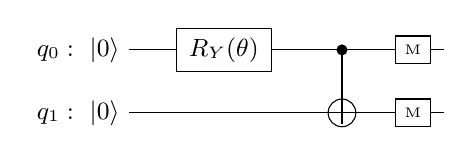
\begin{tikzpicture}[x=1cm, y=0.8cm, font=\small]
\draw (0,0) node[left]{$q_0:\ \ket0$} -- (4,0); \draw (0,-1) node[left]{$q_1:\ \ket0$} -- (4,-1);
\node[draw, fill=white, minimum width=1.2cm] at (1.2,0) {$R_Y(\theta)$};
\fill (2.7,0) circle (2pt); \draw (2.7,0) -- (2.7,-1.18); \draw (2.7,-1) circle (5pt);
\node[draw, fill=white] at (3.6,0) {\tiny M}; \node[draw, fill=white] at (3.6,-1) {\tiny M};
\end{tikzpicture}
\end{center}
Both qubits are then measured in the computational basis; $0 \le \theta \le \pi$.
\end{passagebox}
\needspace{13\baselineskip}
\begin{qitem}{39}
\qmeta{Paragraph based}{Correlations of $R_Y$ + CNOT state}
The expectation values $\langle Z_1\rangle$ and $\langle Z_0Z_1\rangle$ of the final state are
\par\smallskip\noindent\begin{tabularx}{\linewidth}{@{}*{4}{L}@{}}
\correctlabel{A}\,$\cos\theta$ and $1$ & \optlabel{B}\,$1$ and $\cos\theta$ & \optlabel{C}\,$\cos^2(\theta/2)$ and $1$ & \optlabel{D}\,$\cos\theta$ and $\cos^2\theta$
\end{tabularx}
\end{qitem}
\begin{solbox}{A}
\textbf{\color{brand}Correct answer.} \textcolor{okgreen}{\textbf{(A)}} $\cos\theta$ and $1$

\textbf{\color{brand}Concepts required.} Building an entangled state with $R_Y$ + CNOT and computing correlations.

\textbf{\color{brand}Relevant formulae.} $\ket\psi = \cos\frac\theta2\ket{00} + \sin\frac\theta2\ket{11}$; $\langle Z_1\rangle = \sum_{ab}|c_{ab}|^2(-1)^b$, $\langle Z_0Z_1\rangle = \sum|c_{ab}|^2(-1)^{a+b}$.

\textbf{\color{brand}Step-by-step explanation.} $R_Y(\theta)\ket0\otimes\ket0 = \cos\frac\theta2\ket{00} + \sin\frac\theta2\ket{10}$; the CNOT flips qubit 1 when qubit 0 is 1:
$\ket\psi = \cos\frac\theta2\ket{00} + \sin\frac\theta2\ket{11}$.
$\langle Z_1\rangle = \cos^2\frac\theta2 - \sin^2\frac\theta2 = \cos\theta$. Both components have even parity, so
$\langle Z_0Z_1\rangle = 1$ for every $\theta$: the outcomes of the two qubits always agree. (Product of the marginals would give
$\cos^2\theta$, which is wrong because the qubits are correlated.)

\textbf{\color{brand}Why the other options are incorrect.}
\begin{itemize}[leftmargin=2.4em, itemsep=1pt, topsep=2pt]
\item[\textbf{(B)}] $\langle Z_1\rangle = 1$ would mean qubit 1 is always $0$; it is $1$ with probability $\sin^2\frac\theta2$.
\item[\textbf{(C)}] $\cos^2(\theta/2)$ is $P(q_1 = 0)$, not $\langle Z_1\rangle = P(0) - P(1)$.
\item[\textbf{(D)}] $\cos^2\theta$ multiplies the marginals; the outcomes are perfectly correlated, so the parity is always even.
\end{itemize}
\textbf{\color{brand}Key takeaway.} $\langle Z_1\rangle = \cos\theta$, $\langle Z_0Z_1\rangle = 1$: perfectly correlated outcomes.
\end{solbox}
\qsep

\needspace{13\baselineskip}
\begin{qitem}{40}
\qmeta{Paragraph based}{Purity and maximal entanglement}
The value of $\theta$ in $(0, \pi]$ at which the two qubits are \emph{maximally} entangled, and the purity
$\operatorname{tr}\rho_1^2$ of the reduced state of qubit 1 at that value, are
\par\smallskip\noindent\begin{tabularx}{\linewidth}{@{}*{2}{L}@{}}
\optlabel{A}\,$\theta = \pi/2$ and $\operatorname{tr}\rho_1^2 = 1$ & \correctlabel{B}\,$\theta = \pi/2$ and $\operatorname{tr}\rho_1^2 = \tfrac12$ \\[3pt]
\optlabel{C}\,$\theta = \pi$ and $\operatorname{tr}\rho_1^2 = \tfrac12$ & \optlabel{D}\,$\theta = \pi/4$ and $\operatorname{tr}\rho_1^2 = \tfrac34$
\end{tabularx}
\end{qitem}
\begin{solbox}{B}
\textbf{\color{brand}Correct answer.} \textcolor{okgreen}{\textbf{(B)}} $\theta = \pi/2$ and $\operatorname{tr}\rho_1^2 = \tfrac12$

\textbf{\color{brand}Concepts required.} Entanglement of a pure bipartite state measured by the mixedness (purity) of the reduced state.

\textbf{\color{brand}Relevant formulae.} $\rho_1 = \operatorname{diag}(\cos^2\frac\theta2, \sin^2\frac\theta2)$; $\operatorname{tr}\rho_1^2 = \frac{1 + \cos^2\theta}{2} \in [\frac12, 1]$.

\textbf{\color{brand}Step-by-step explanation.} Tracing out qubit 0 from $\cos\frac\theta2\ket{00} + \sin\frac\theta2\ket{11}$ gives $\rho_1 = \operatorname{diag}(\cos^2\frac\theta2, \sin^2\frac\theta2)$
and purity $\operatorname{tr}\rho_1^2 = \cos^4\frac\theta2 + \sin^4\frac\theta2 = \frac{1 + \cos^2\theta}{2}$. It is minimal (most mixed,
most entangled) when $\cos\theta = 0$: $\theta = \frac\pi2$, giving $\frac12$ --- the Bell state $\ket{\Phi^+}$.
At $\theta = \pi$ the state is $\ket{11}$ (product, purity 1); at $\theta = \frac\pi4$ the purity is $\frac{1 + 1/2}{2} = \frac34$.

\textbf{\color{brand}Why the other options are incorrect.}
\begin{itemize}[leftmargin=2.4em, itemsep=1pt, topsep=2pt]
\item[\textbf{(A)}] Purity 1 means a pure reduced state, i.e.\ \emph{no} entanglement.
\item[\textbf{(C)}] $\theta = \pi$ gives $\ket{11}$, a product state with purity 1.
\item[\textbf{(D)}] At $\theta = \frac\pi4$ the state is only partially entangled (purity $\frac34$).
\end{itemize}
\textbf{\color{brand}Key takeaway.} Maximal entanglement $\Leftrightarrow$ maximally mixed reduced state ($\operatorname{tr}\rho^2 = \frac12$ for a qubit).
\end{solbox}
\qsep

\newpage

\begin{sectionbanner}SECTION C \enspace$\cdot$\enspace Quantum Machine Learning Fundamentals \hfill Q.41--60\end{sectionbanner}

\needspace{13\baselineskip}
\begin{qitem}{41}
\qmeta{Single-correct MCQ}{Angle encoding of a pixel}
\texttt{QML.ipynb} encodes a pixel value $x \in [0, 1]$ with \texttt{ry(np.pi * x, q)} on a qubit in $\ket0$. For a
pixel of brightness $x = \frac13$ the probability of measuring $1$ on that qubit and its $\langle Z\rangle$ (before any other gate) are
\par\smallskip\noindent\begin{tabularx}{\linewidth}{@{}*{2}{L}@{}}
\correctlabel{A}\,$P(1) = \frac14$, $\langle Z\rangle = \frac12$ & \optlabel{B}\,$P(1) = \frac12$, $\langle Z\rangle = 0$ \\[3pt]
\optlabel{C}\,$P(1) = \frac13$, $\langle Z\rangle = \frac13$ & \optlabel{D}\,$P(1) = \frac34$, $\langle Z\rangle = -\frac12$
\end{tabularx}
\end{qitem}
\begin{solbox}{A}
\textbf{\color{brand}Correct answer.} \textcolor{okgreen}{\textbf{(A)}} $P(1) = \frac14$, $\langle Z\rangle = \frac12$

\textbf{\color{brand}Concepts required.} Angle encoding writes a feature into a rotation angle; the half-angle appears in the amplitudes.

\textbf{\color{brand}Relevant formulae.} $R_Y(\pi x)\ket0 = \cos\frac{\pi x}2\ket0 + \sin\frac{\pi x}2\ket1$; $P(1) = \sin^2\frac{\pi x}2$, $\langle Z\rangle = \cos\pi x$.

\textbf{\color{brand}Step-by-step explanation.} $R_Y(\pi x)\ket0 = \cos\frac{\pi x}{2}\ket0 + \sin\frac{\pi x}{2}\ket1$. For $x = \frac13$ the half-angle is $\frac\pi6$:
$P(1) = \sin^2\frac\pi6 = \frac14$, $P(0) = \frac34$, so $\langle Z\rangle = \frac34 - \frac14 = \frac12 = \cos\frac\pi3 = \cos(\pi x)$.
A dark pixel ($x = 0$) stays $\ket0$, a lit pixel ($x = 1$) becomes $\ket1$, intermediate values give superpositions.

\textbf{\color{brand}Why the other options are incorrect.}
\begin{itemize}[leftmargin=2.4em, itemsep=1pt, topsep=2pt]
\item[\textbf{(B)}] $P(1) = \frac12$ would correspond to $x = \frac12$.
\item[\textbf{(C)}] Angle encoding does not make $P(1)$ equal to the pixel value; $P(1) = \sin^2\frac{\pi x}{2}$ is non-linear in $x$.
\item[\textbf{(D)}] $P(1) = \frac34$ uses $\sin^2(\pi x)$, forgetting the half-angle of $R_Y$.
\end{itemize}
\textbf{\color{brand}Key takeaway.} Notebook encoding: $\langle Z_i\rangle = \cos(\pi x_i)$ before the QCNN layers.
\end{solbox}
\qsep

\needspace{13\baselineskip}
\begin{qitem}{42}
\qmeta{Single-correct MCQ}{Amplitude encoding}
The vector $\mathbf x = (1, 2, 4, 2)$ is amplitude-encoded: $\ket{\psi_{\mathbf x}} = \sum_j \frac{x_j}{\|\mathbf x\|}\ket j$ with
$\ket0 = \ket{00}, \ket1 = \ket{01}, \ket2 = \ket{10}, \ket3 = \ket{11}$ (qubit 0 written first). The number of qubits and the
probability that a measurement of qubit 0 gives 1 are
\par\smallskip\noindent\begin{tabularx}{\linewidth}{@{}*{4}{L}@{}}
\optlabel{A}\,$2$ qubits; $0.32$ & \optlabel{B}\,$2$ qubits; $0.60$ & \optlabel{C}\,$4$ qubits; $0.80$ & \correctlabel{D}\,$2$ qubits; $0.80$
\end{tabularx}
\end{qitem}
\begin{solbox}{D}
\textbf{\color{brand}Correct answer.} \textcolor{okgreen}{\textbf{(D)}} $2$ qubits; $0.80$

\textbf{\color{brand}Concepts required.} Amplitude encoding stores a normalised vector in the amplitudes of $\log_2d$ qubits.

\textbf{\color{brand}Relevant formulae.} $\ket{\psi_{\mathbf x}} = \frac{1}{\|\mathbf x\|}\sum_jx_j\ket j$; $P(q_0 = 1) = \sum_{j:\,q_0(j) = 1}|x_j|^2/\|\mathbf x\|^2$.

\textbf{\color{brand}Step-by-step explanation.} Four amplitudes need $\log_2 4 = 2$ qubits. $\|\mathbf x\| = \sqrt{1 + 4 + 16 + 4} = 5$, so the amplitudes are
$(0.2, 0.4, 0.8, 0.4)$ on $\ket{00}, \ket{01}, \ket{10}, \ket{11}$. Qubit 0 is 1 in $\ket{10}$ and $\ket{11}$:
$P = 0.8^2 + 0.4^2 = 0.64 + 0.16 = 0.80$. (Qubit 1 is 1 in $\ket{01}, \ket{11}$: $0.16 + 0.16 = 0.32$.) Amplitude encoding is
exponentially compact in qubits, but preparing a general such state needs $O(2^n)$ gates.

\textbf{\color{brand}Why the other options are incorrect.}
\begin{itemize}[leftmargin=2.4em, itemsep=1pt, topsep=2pt]
\item[\textbf{(A)}] $0.32$ is the probability for qubit 1 (basis states $\ket{01}, \ket{11}$), not qubit 0.
\item[\textbf{(B)}] $0.60$ averages the amplitudes $0.8$ and $0.4$ instead of adding their squares.
\item[\textbf{(C)}] Four qubits would be angle/basis encoding; amplitude encoding needs only $\log_24 = 2$.
\end{itemize}
\textbf{\color{brand}Key takeaway.} Normalise, then sum $|$amplitude$|^2$ over the basis states with the wanted bit.
\end{solbox}
\qsep

\needspace{13\baselineskip}
\begin{qitem}{43}
\qmeta{Single-correct MCQ}{Qubit cost of encodings}
A data point has $d = 256$ real features, each stored with 8-bit precision. The numbers of qubits needed by
\emph{basis} encoding (every bit on its own qubit), \emph{angle} encoding (one feature per qubit) and \emph{amplitude} encoding are
\par\smallskip\noindent\begin{tabularx}{\linewidth}{@{}*{4}{L}@{}}
\optlabel{A}\,$256$, $256$, $8$ & \optlabel{B}\,$8$, $256$, $2048$ & \correctlabel{C}\,$2048$, $256$, $8$ & \optlabel{D}\,$2048$, $8$, $256$
\end{tabularx}
\end{qitem}
\begin{solbox}{C}
\textbf{\color{brand}Correct answer.} \textcolor{okgreen}{\textbf{(C)}} $2048$, $256$, $8$

\textbf{\color{brand}Concepts required.} Resource comparison of basis, angle and amplitude encoding.

\textbf{\color{brand}Relevant formulae.} Qubits: basis $= d\cdot b$ ($b$ bits per feature), angle $= d$, amplitude $= \lceil\log_2d\rceil$.

\textbf{\color{brand}Step-by-step explanation.} Basis encoding writes the bit string into computational basis states: $256 \times 8 = 2048$ bits, one qubit each.
Angle encoding uses one rotation angle per feature: $256$ qubits. Amplitude encoding stores $256 = 2^8$ numbers as the
amplitudes of $8$ qubits. Fewer qubits come at the price of a deeper, more complicated state-preparation circuit.

\textbf{\color{brand}Why the other options are incorrect.}
\begin{itemize}[leftmargin=2.4em, itemsep=1pt, topsep=2pt]
\item[\textbf{(A)}] $256$ basis qubits ignores the 8 bits per feature.
\item[\textbf{(B)}] The order is reversed: basis encoding is the most qubit-hungry, amplitude the least.
\item[\textbf{(D)}] Angle and amplitude are swapped: angle encoding is linear in $d$, amplitude encoding logarithmic.
\end{itemize}
\textbf{\color{brand}Key takeaway.} Qubits: basis $\gg$ angle $\gg$ amplitude; circuit depth runs the other way.
\end{solbox}
\qsep

\needspace{13\baselineskip}
\begin{qitem}{44}
\qmeta{Single-correct MCQ}{Fidelity kernel of angle encoding}
With the notebook's angle encoding $\ket{\psi(\mathbf x)} = \bigotimes_i R_Y(\pi x_i)\ket0$, the fidelity (quantum) kernel
$k(\mathbf x, \mathbf x') = |\braket{\psi(\mathbf x)|\psi(\mathbf x')}|^2$ for $\mathbf x = (1, 0.5)$ and $\mathbf x' = (0.5, 0)$ is
\par\smallskip\noindent\begin{tabularx}{\linewidth}{@{}*{4}{L}@{}}
\optlabel{A}\,$\frac1{16}$ & \correctlabel{B}\,$\frac14$ & \optlabel{C}\,$\frac12$ & \optlabel{D}\,$0$
\end{tabularx}
\end{qitem}
\begin{solbox}{B}
\textbf{\color{brand}Correct answer.} \textcolor{okgreen}{\textbf{(B)}} $\frac14$

\textbf{\color{brand}Concepts required.} Fidelity kernel of a product (angle) encoding factorises over qubits.

\textbf{\color{brand}Relevant formulae.} $\braket{\psi(x)|\psi(x')} = \cos\frac{\pi(x - x')}{2}$ per qubit; $k = \prod_i\cos^2\frac{\pi(x_i - x'_i)}{2}$.

\textbf{\color{brand}Step-by-step explanation.} For one qubit $\braket{\psi(x)|\psi(x')} = \cos\frac{\pi x}{2}\cos\frac{\pi x'}{2} + \sin\frac{\pi x}{2}\sin\frac{\pi x'}{2} = \cos\frac{\pi(x - x')}{2}$.
For a product state the overlap is the product: $k = \prod_i\cos^2\frac{\pi(x_i - x'_i)}{2}$.
Here $x_0 - x'_0 = 0.5$ and $x_1 - x'_1 = 0.5$, so $k = \cos^2\frac\pi4\cdot\cos^2\frac\pi4 = \frac12\cdot\frac12 = \frac14$.
(The overlap itself is $\frac12$; the kernel is its square.) Note that this kernel has a simple closed form --- it can be evaluated
classically in $O(d)$ time.

\textbf{\color{brand}Why the other options are incorrect.}
\begin{itemize}[leftmargin=2.4em, itemsep=1pt, topsep=2pt]
\item[\textbf{(A)}] $\frac1{16}$ squares the kernel again ($|\braket{\psi|\psi'}|^4$).
\item[\textbf{(C)}] $\frac12$ is the overlap $|\braket{\psi|\psi'}|$, not its square.
\item[\textbf{(D)}] $0$ would need orthogonal states, i.e.\ a feature difference of 1 on some qubit.
\end{itemize}
\textbf{\color{brand}Key takeaway.} Product encodings give product kernels --- classically cheap, so no quantum advantage from them.
\end{solbox}
\qsep

\needspace{13\baselineskip}
\begin{qitem}{45}
\qmeta{Single-correct MCQ}{Size of the kernel computation}
A quantum-kernel SVM is trained on $M = 20$ points. Every kernel entry $k_{ij} = |\braket{\psi_i|\psi_j}|^2$, with $\ket{\psi_i} = \ket{\psi(\mathbf x_i)}$,
is estimated by its own circuit. Using $k(\mathbf x, \mathbf x) = 1$ and the symmetry $k_{ij} = k_{ji}$, the number of distinct
circuits needed for the training Gram matrix is
\par\smallskip\noindent\begin{tabularx}{\linewidth}{@{}*{4}{L}@{}}
\correctlabel{A}\,$190$ & \optlabel{B}\,$400$ & \optlabel{C}\,$380$ & \optlabel{D}\,$20$
\end{tabularx}
\end{qitem}
\begin{solbox}{A}
\textbf{\color{brand}Correct answer.} \textcolor{okgreen}{\textbf{(A)}} $190$

\textbf{\color{brand}Concepts required.} Cost of building a kernel (Gram) matrix with a quantum computer.

\textbf{\color{brand}Relevant formulae.} Distinct off-diagonal entries of a symmetric $M\times M$ matrix: $\binom M2 = \frac{M(M-1)}{2}$.

\textbf{\color{brand}Step-by-step explanation.} The $20\times20$ Gram matrix has $400$ entries. The $20$ diagonal entries are known ($=1$), leaving $380$
off-diagonal entries, and symmetry halves them: $\binom{20}{2} = \frac{20\cdot19}{2} = 190$ circuits (each run with many shots).
Prediction on a new point needs another $M = 20$ kernel values. The quadratic growth $O(M^2)$ is a practical limitation of kernel methods.

\textbf{\color{brand}Why the other options are incorrect.}
\begin{itemize}[leftmargin=2.4em, itemsep=1pt, topsep=2pt]
\item[\textbf{(B)}] $400 = M^2$ ignores the known diagonal and the symmetry.
\item[\textbf{(C)}] $380 = M^2 - M$ ignores the symmetry $k_{ij} = k_{ji}$.
\item[\textbf{(D)}] $20$ counts the training points, not the pairs.
\end{itemize}
\textbf{\color{brand}Key takeaway.} Kernel training needs $O(M^2)$ circuit estimates; prediction $O(M)$ per new point.
\end{solbox}
\qsep

\needspace{13\baselineskip}
\begin{qitem}{46}
\qmeta{Single-correct MCQ}{Swap test}
In a swap test between the states $\ket\psi$ and $\ket\phi$ the ancilla is measured in state $0$ with probability $0.8$.
The fidelity kernel $|\braket{\psi|\phi}|^2$ is
\par\smallskip\noindent\begin{tabularx}{\linewidth}{@{}*{4}{L}@{}}
\optlabel{A}\,$0.3$ & \optlabel{B}\,$0.8$ & \optlabel{C}\,$0.89$ & \correctlabel{D}\,$0.6$
\end{tabularx}
\end{qitem}
\begin{solbox}{D}
\textbf{\color{brand}Correct answer.} \textcolor{okgreen}{\textbf{(D)}} $0.6$

\textbf{\color{brand}Concepts required.} The swap test estimates the squared overlap of two states from one ancilla qubit.

\textbf{\color{brand}Relevant formulae.} $P(\text{ancilla} = 0) = \frac12(1 + |\braket{\psi|\phi}|^2)$.

\textbf{\color{brand}Step-by-step explanation.} The swap test (Hadamard on the ancilla, controlled-SWAP, Hadamard, measure) gives
$P(0) = \frac12\big(1 + |\braket{\psi|\phi}|^2\big)$. Solving: $|\braket{\psi|\phi}|^2 = 2P(0) - 1 = 2(0.8) - 1 = 0.6$.
Orthogonal states give $P(0) = \frac12$, identical states $P(0) = 1$. (The compute--uncompute test $U(\mathbf x')^\dagger U(\mathbf x)$
instead gives $|\braket{\psi|\phi}|^2$ directly as the probability of the all-zero outcome.)

\textbf{\color{brand}Why the other options are incorrect.}
\begin{itemize}[leftmargin=2.4em, itemsep=1pt, topsep=2pt]
\item[\textbf{(A)}] $0.3$ uses $P(0) - \frac12$ without the factor 2.
\item[\textbf{(B)}] $0.8$ is $P(0)$ itself, not the overlap.
\item[\textbf{(C)}] $0.89 = \sqrt{0.8}$ has no meaning here.
\end{itemize}
\textbf{\color{brand}Key takeaway.} $|\braket{\psi|\phi}|^2 = 2P(0) - 1$.
\end{solbox}
\qsep

\needspace{13\baselineskip}
\begin{qitem}{47}
\qmeta{Single-correct MCQ}{Two-term parameter-shift rule}
A parameter $\theta$ enters a circuit only through one gate $R_Y(\theta)$. The measured expectation values are
$f(\theta + \frac\pi2) = 0.30$ and $f(\theta - \frac\pi2) = -0.50$. The exact derivative $f'(\theta)$ is
\par\smallskip\noindent\begin{tabularx}{\linewidth}{@{}*{4}{L}@{}}
\optlabel{A}\,$-0.40$ & \optlabel{B}\,$0.25$ & \correctlabel{C}\,$0.40$ & \optlabel{D}\,$0.80$
\end{tabularx}
\end{qitem}
\begin{solbox}{C}
\textbf{\color{brand}Correct answer.} \textcolor{okgreen}{\textbf{(C)}} $0.40$

\textbf{\color{brand}Concepts required.} The parameter-shift rule gives exact derivatives of expectation values for Pauli-rotation gates.

\textbf{\color{brand}Relevant formulae.} $f'(\theta) = \frac12[f(\theta + \frac\pi2) - f(\theta - \frac\pi2)]$ for a gate $e^{-i\theta P/2}$, $P^2 = I$.

\textbf{\color{brand}Step-by-step explanation.} The two-term parameter-shift rule for a gate $e^{-i\theta P/2}$ ($P$ a Pauli operator) is
$f'(\theta) = \frac12\big[f(\theta + \frac\pi2) - f(\theta - \frac\pi2)\big]$. Here $\frac12(0.30 - (-0.50)) = 0.40$.
The rule is \emph{exact} (no step-size error), because $f(\theta) = a + b\cos\theta + c\sin\theta$:
$\frac12[f(\theta + \frac\pi2) - f(\theta - \frac\pi2)] = \frac12[-2b\sin\theta + 2c\cos\theta] = f'(\theta)$.

\textbf{\color{brand}Why the other options are incorrect.}
\begin{itemize}[leftmargin=2.4em, itemsep=1pt, topsep=2pt]
\item[\textbf{(A)}] $-0.40$ subtracts in the wrong order.
\item[\textbf{(B)}] $0.25 \approx 0.8/\pi$ treats the shifts as a finite difference with step $\pi$, which is not how the rule works.
\item[\textbf{(D)}] $0.80$ forgets the factor $\frac12$.
\end{itemize}
\textbf{\color{brand}Key takeaway.} Two circuit runs, shifted by $\pm\frac\pi2$, give the exact derivative --- no step-size error.
\end{solbox}
\qsep

\needspace{13\baselineskip}
\begin{qitem}{48}
\qmeta{Single-correct MCQ}{Shared parameters in the QCNN}
In the default 8-qubit QCNN of \texttt{QML.ipynb}, the parameter $\theta_{1,1}$ = \texttt{theta[0]} is used by how many
$R_Y$ gates, and how many circuit evaluations does an exact parameter-shift derivative with respect to it need for one image
(shifting each occurrence separately)?
\par\smallskip\noindent\begin{tabularx}{\linewidth}{@{}*{2}{L}@{}}
\optlabel{A}\,$11$ gates; $22$ circuits & \optlabel{B}\,$4$ gates; $8$ circuits \\[3pt]
\correctlabel{C}\,$7$ gates; $14$ circuits & \optlabel{D}\,$1$ gate; $2$ circuits
\end{tabularx}
\end{qitem}
\begin{solbox}{C}
\textbf{\color{brand}Correct answer.} \textcolor{okgreen}{\textbf{(C)}} $7$ gates; $14$ circuits

\textbf{\color{brand}Concepts required.} Weight sharing: one parameter in many gates; the derivative is the sum over occurrences (product rule).

\textbf{\color{brand}Relevant formulae.} $\partial_\theta f = \sum_g\partial_{\theta^{(g)}}f$; each $R_Y$ occurrence: 2 shifted circuits.

\textbf{\color{brand}Step-by-step explanation.} \texttt{theta[0]} is the first parameter of layer 1; it is applied by \texttt{ry(theta[t], qubits[a])} in \emph{every}
convolution block of that layer. Layer 1 acts on all 8 qubits: pairs $(0,1), (2,3), (4,5), (6,7)$ and then $(1,2), (3,4), (5,6)$,
i.e.\ $4 + 3 = 7$ blocks, so 7 gates share $\theta_{1,1}$ (weight sharing, as in a CNN filter). By the product rule
$\partial_\theta f = \sum_{g=1}^{7}\partial_{\theta^{(g)}} f$, and each occurrence needs the two-term shift (2 circuits):
$7\times2 = 14$ circuits. Shifting the shared value once (2 circuits) does \emph{not} give the derivative.

\textbf{\color{brand}Why the other options are incorrect.}
\begin{itemize}[leftmargin=2.4em, itemsep=1pt, topsep=2pt]
\item[\textbf{(A)}] $11$ counts the convolution blocks of \emph{all} layers; layers 2 and 3 use \texttt{theta[4]} and \texttt{theta[8]} instead.
\item[\textbf{(B)}] $4$ counts only the even pairs $(0,1), (2,3), (4,5), (6,7)$ and forgets the odd pairs $(1,2), (3,4), (5,6)$.
\item[\textbf{(D)}] One gate would hold without weight sharing; in the QCNN every convolution block of layer 1 uses \texttt{theta[0]}.
\end{itemize}
\textbf{\color{brand}Key takeaway.} Shared parameters need one shift pair per occurrence: $7\times2 = 14$ circuits for $\theta_{1,1}$.
\end{solbox}
\qsep

\needspace{13\baselineskip}
\begin{qitem}{49}
\qmeta{Single-correct MCQ}{QCNN depth and parameters}
Using the notebook's layout rule (pool pairs of active qubits, keep the sinks; an odd last qubit moves on unchanged;
4 parameters per layer), a QCNN on $N = 20$ qubits (e.g.\ $4\times5$ pixels) has
\par\smallskip\noindent\begin{tabularx}{\linewidth}{@{}*{2}{L}@{}}
\optlabel{A}\,$4$ layers and $16$ parameters & \optlabel{B}\,$19$ layers and $76$ parameters \\[3pt]
\optlabel{C}\,$5$ layers and $40$ parameters & \correctlabel{D}\,$5$ layers and $20$ parameters
\end{tabularx}
\end{qitem}
\begin{solbox}{D}
\textbf{\color{brand}Correct answer.} \textcolor{okgreen}{\textbf{(D)}} $5$ layers and $20$ parameters

\textbf{\color{brand}Concepts required.} QCNN depth: pooling halves (rounding up) the number of active qubits until one remains.

\textbf{\color{brand}Relevant formulae.} $n \to \lceil n/2\rceil$ per layer; layers $= \lceil\log_2N\rceil$; parameters $= 4\times$layers.

\textbf{\color{brand}Step-by-step explanation.} Track the number of active qubits: pooling keeps $\lceil n/2\rceil$ of $n$ (the sinks, plus the odd last qubit).
$20 \to 10 \to 5 \to 3 \to 2 \to 1$: five layers. With four shared parameters per layer: $4\times5 = 20$ parameters.
In general the layer count is $\lceil\log_2 N\rceil$ and the parameter count $4\lceil\log_2 N\rceil$ --- logarithmic in $N$, while a
dense classical layer on $N$ inputs has $O(N)$ weights.

\textbf{\color{brand}Why the other options are incorrect.}
\begin{itemize}[leftmargin=2.4em, itemsep=1pt, topsep=2pt]
\item[\textbf{(A)}] $4$ layers would leave 2 qubits from 20 ($20\to10\to5\to3\to2$); one more pooling is needed.
\item[\textbf{(B)}] $19$ layers would pool away one qubit per layer; the QCNN halves the register.
\item[\textbf{(C)}] $40$ parameters counts 8 per layer; each layer has only 4 shared parameters.
\end{itemize}
\textbf{\color{brand}Key takeaway.} $20 \to 10 \to 5 \to 3 \to 2 \to 1$: 5 layers, 20 parameters.
\end{solbox}
\qsep

\needspace{13\baselineskip}
\begin{qitem}{50}
\qmeta{Single-correct MCQ}{Pooling block (code)}
The pooling block of \texttt{QML.ipynb} on source qubit $a$ and sink qubit $b$ is
\texttt{rz.ctrl(t3, q[a], q[b]); x(q[a]); rx.ctrl(t4, q[a], q[b]); x(q[a])}. As an operator it equals
\par\smallskip\noindent\begin{tabularx}{\linewidth}{@{}*{2}{L}@{}}
\optlabel{A}\,$R_Z(t_3)_b\,R_X(t_4)_b$ (independent of qubit $a$) & \optlabel{B}\,$\ket1\!\bra1_b\otimes R_Z(t_3)_a + \ket0\!\bra0_b\otimes R_X(t_4)_a$ \\[3pt]
\optlabel{C}\,$\ket0\!\bra0_a\otimes R_Z(t_3)_b + \ket1\!\bra1_a\otimes R_X(t_4)_b$ & \correctlabel{D}\,$\ket1\!\bra1_a\otimes R_Z(t_3)_b + \ket0\!\bra0_a\otimes R_X(t_4)_b$
\end{tabularx}
\end{qitem}
\begin{solbox}{D}
\textbf{\color{brand}Correct answer.} \textcolor{okgreen}{\textbf{(D)}} $\ket1\!\bra1_a\otimes R_Z(t_3)_b + \ket0\!\bra0_a\otimes R_X(t_4)_b$

\textbf{\color{brand}Concepts required.} Reading CUDA-Q code: \texttt{x}-conjugation turns a controlled gate into an anti-controlled one.

\textbf{\color{brand}Relevant formulae.} $(X\otimes I)\,C\text{-}U\,(X\otimes I) = \ket1\!\bra1\otimes I + \ket0\!\bra0\otimes U$.

\textbf{\color{brand}Step-by-step explanation.} \texttt{rz.ctrl(t3, q[a], q[b])} $= \ket0\!\bra0_a\otimes I + \ket1\!\bra1_a\otimes R_Z(t_3)$. The pair \texttt{x(q[a]) \dots\ x(q[a])}
turns the following controlled gate into an \emph{anti}-controlled one (it acts when $a$ is $\ket0$):
$\ket1\!\bra1_a\otimes I + \ket0\!\bra0_a\otimes R_X(t_4)$. Multiplying the two (they act on orthogonal control subspaces):
$\ket1\!\bra1_a\otimes R_Z(t_3) + \ket0\!\bra0_a\otimes R_X(t_4)$. Qubit $a$ is never used again; by the deferred-measurement
principle this equals ``measure $a$, then rotate $b$ according to the result''.

\textbf{\color{brand}Why the other options are incorrect.}
\begin{itemize}[leftmargin=2.4em, itemsep=1pt, topsep=2pt]
\item[\textbf{(A)}] The rotations are controlled; on their own they would not depend on the source qubit at all.
\item[\textbf{(B)}] Source and sink are swapped: \texttt{q[a]} is the control, \texttt{q[b]} the target.
\item[\textbf{(C)}] This swaps the roles: \texttt{rz.ctrl} without the $X$ sandwich acts when $a$ is $\ket1$.
\end{itemize}
\textbf{\color{brand}Key takeaway.} Pooling = ``if $a = 1$ rotate $b$ about $Z$, else about $X$'', then forget $a$.
\end{solbox}
\qsep

\needspace{13\baselineskip}
\begin{qitem}{51}
\qmeta{Single-correct MCQ}{QCNN gate count}
For $N = 16$ qubits the notebook's layout has $26$ convolution blocks and $15$ pooling blocks. Counting the $N$
encoding rotations and every gate of the blocks as \texttt{cudaq.estimate\_resources} does, the circuit has
\par\smallskip\noindent\begin{tabularx}{\linewidth}{@{}*{4}{L}@{}}
\optlabel{A}\,$138$ gates & \correctlabel{B}\,$154$ gates & \optlabel{C}\,$124$ gates & \optlabel{D}\,$170$ gates
\end{tabularx}
\end{qitem}
\begin{solbox}{B}
\textbf{\color{brand}Correct answer.} \textcolor{okgreen}{\textbf{(B)}} $154$ gates

\textbf{\color{brand}Concepts required.} Counting gates from the layout: encoding + blocks.

\textbf{\color{brand}Relevant formulae.} Gates $= N + 3n_{\text{conv}} + 4n_{\text{pool}}$ (conv: 2 \texttt{ry} + \texttt{cx}; pool: \texttt{crz}, 2 \texttt{x}, \texttt{crx}).

\textbf{\color{brand}Step-by-step explanation.} Per convolution block: 2 \texttt{ry} + 1 CNOT = 3 gates. Per pooling block: \texttt{crz}, \texttt{x}, \texttt{crx}, \texttt{x} = 4 gates.
Total $= N + 3n_{\text{conv}} + 4n_{\text{pool}} = 16 + 3(26) + 4(15) = 16 + 78 + 60 = 154$.
\emph{Check} with the default: $8 + 3(11) + 4(7) = 8 + 33 + 28 = 69$, the recorded value. (Doubling 69 gives 138, but the
block counts do not scale linearly.)

\textbf{\color{brand}Why the other options are incorrect.}
\begin{itemize}[leftmargin=2.4em, itemsep=1pt, topsep=2pt]
\item[\textbf{(A)}] $138$ doubles the 8-qubit count; block counts grow as $\approx 2N$ and $N$, not exactly by a factor 2.
\item[\textbf{(C)}] $124$ forgets the two $X$ gates of every pooling block.
\item[\textbf{(D)}] $170$ counts the 16 encoding rotations twice.
\end{itemize}
\textbf{\color{brand}Key takeaway.} $16 + 78 + 60 = 154$; the formula reproduces the recorded 69 gates at $N = 8$.
\end{solbox}
\qsep

\needspace{13\baselineskip}
\begin{qitem}{52}
\qmeta{Single-correct MCQ}{MSE vs.\ accuracy}
A classifier with outputs in $[-1, 1]$ and prediction $\operatorname{sign} f$ gives $f = 0.6,\ -0.2,\ 0.9,\ 0.1$ on four
images with labels $y = +1,\ -1,\ +1,\ -1$. Its mean squared error (as in \texttt{QML.ipynb}) and accuracy are
\par\smallskip\noindent\begin{tabularx}{\linewidth}{@{}*{4}{L}@{}}
\correctlabel{A}\,$0.505$ and $75\,\%$ & \optlabel{B}\,$2.02$ and $75\,\%$ & \optlabel{C}\,$0.60$ and $75\,\%$ & \optlabel{D}\,$0.505$ and $50\,\%$
\end{tabularx}
\end{qitem}
\begin{solbox}{A}
\textbf{\color{brand}Correct answer.} \textcolor{okgreen}{\textbf{(A)}} $0.505$ and $75\,\%$

\textbf{\color{brand}Concepts required.} MSE on real-valued outputs vs.\ sign-based accuracy.

\textbf{\color{brand}Relevant formulae.} $\mathcal L = \frac1M\sum(f_m - y_m)^2$; accuracy $= \frac1M\#\{m: \operatorname{sign}f_m = y_m\}$.

\textbf{\color{brand}Step-by-step explanation.} Errors $f - y$: $-0.4,\ 0.8,\ -0.1,\ 1.1$; squares $0.16,\ 0.64,\ 0.01,\ 1.21$; sum $2.02$; mean $\mathcal L = 0.505$.
Signs: $+, -, +, +$ against labels $+, -, +, -$: three correct, accuracy $75\,\%$. The second image is classified correctly even
though its error is large ($0.8$): MSE punishes small margins, accuracy only looks at the sign.

\textbf{\color{brand}Why the other options are incorrect.}
\begin{itemize}[leftmargin=2.4em, itemsep=1pt, topsep=2pt]
\item[\textbf{(B)}] $2.02$ is the sum of squared errors, not the mean.
\item[\textbf{(C)}] $0.60$ is the mean \emph{absolute} error.
\item[\textbf{(D)}] $50\,\%$ counts the second image as wrong; $\operatorname{sign}(-0.2) = -1 = y$, correct.
\end{itemize}
\textbf{\color{brand}Key takeaway.} A correct sign with a small margin still costs MSE.
\end{solbox}
\qsep

\needspace{13\baselineskip}
\begin{qitem}{53}
\qmeta{Single-correct MCQ}{Circuit count and run time of the notebook}
With its defaults (20 training images, \texttt{MAX\_ITERATIONS = 100} loss evaluations, 20 test images) and the
recorded time of $1.7$ ms per circuit on \texttt{qpp-cpu}, the number of circuits \texttt{QML.ipynb} runs for training plus testing
and the resulting estimate of the run time are
\par\smallskip\noindent\begin{tabularx}{\linewidth}{@{}*{2}{L}@{}}
\correctlabel{A}\,$2020$ circuits, about $3.4$ s & \optlabel{B}\,$100$ circuits, about $0.17$ s \\[3pt]
\optlabel{C}\,$2020$ circuits, about $34$ s & \optlabel{D}\,$2000$ circuits, about $0.17$ s
\end{tabularx}
\end{qitem}
\begin{solbox}{A}
\textbf{\color{brand}Correct answer.} \textcolor{okgreen}{\textbf{(A)}} $2020$ circuits, about $3.4$ s

\textbf{\color{brand}Concepts required.} Cost model of hybrid training: circuits per loss evaluation = number of training images.

\textbf{\color{brand}Relevant formulae.} Circuits $= M_{\text{train}}\times n_{\text{eval}} + M_{\text{test}}$; time $\approx$ circuits $\times$ time per circuit.

\textbf{\color{brand}Step-by-step explanation.} Every loss evaluation runs the QCNN once per training image: $100\times20 = 2000$ circuits; evaluating the test set adds 20:
$2020$ circuits (the notebook prints exactly this number). Time: $2020\times1.7\ \text{ms} = 3.43$ s; the recorded training time was
$3.4$ s. The classical optimizer itself costs almost nothing --- simulation dominates.

\textbf{\color{brand}Why the other options are incorrect.}
\begin{itemize}[leftmargin=2.4em, itemsep=1pt, topsep=2pt]
\item[\textbf{(B)}] $100$ circuits counts loss evaluations, but each evaluation runs one circuit per image.
\item[\textbf{(C)}] $34$ s is ten times too large ($2020\times1.7\ \text{ms} = 3.4$ s).
\item[\textbf{(D)}] $2000$ circuits forgets the 20 test circuits, and $0.17$ s is $100\times1.7$ ms.
\end{itemize}
\textbf{\color{brand}Key takeaway.} $2020\times1.7$ ms $\approx 3.4$ s --- the recorded training time.
\end{solbox}
\qsep

\needspace{13\baselineskip}
\begin{qitem}{54}
\qmeta{Single-correct MCQ}{Data re-uploading frequencies}
A single-qubit model alternates trainable unitaries with the data-encoding gate $R_Y(x)$, which appears $L = 3$ times
(``data re-uploading''). Its output $f(x) = \langle Z\rangle$ is a trigonometric series in $x$. The highest frequency it can contain is
\par\smallskip\noindent\begin{tabularx}{\linewidth}{@{}*{4}{L}@{}}
\optlabel{A}\,$8$ & \correctlabel{B}\,$3$ & \optlabel{C}\,$1$ & \optlabel{D}\,$6$
\end{tabularx}
\end{qitem}
\begin{solbox}{B}
\textbf{\color{brand}Correct answer.} \textcolor{okgreen}{\textbf{(B)}} $3$

\textbf{\color{brand}Concepts required.} Frequency spectrum of quantum models; data re-uploading.

\textbf{\color{brand}Relevant formulae.} $f(x) = \sum_{\omega\in\Omega}c_\omega e^{i\omega x}$ with $\Omega = \{\lambda_j - \lambda_k\}$ of the sums of generator eigenvalues; $L$ uses of $e^{-ixY/2}$: $\Omega = \{-L, \dots, L\}$.

\textbf{\color{brand}Step-by-step explanation.} Each $R_Y(x) = e^{-ixY/2}$ has generator eigenvalues $\pm\frac12$. In $f = \braket{\psi|M|\psi}$ each occurrence contributes
phases $e^{\pm ix/2}$ from the ket and from the bra; with $L$ occurrences the exponents are differences of sums of $L$ terms $\pm\frac12$,
so the frequencies are the integers $0, 1, \dots, L$ (Schuld, Sweke \& Meyer 2021). With one encoding gate $f(x) = a + b\cos x + c\sin x$;
with $L = 3$ the spectrum reaches frequency 3. Repeating the encoding increases expressivity.

\textbf{\color{brand}Why the other options are incorrect.}
\begin{itemize}[leftmargin=2.4em, itemsep=1pt, topsep=2pt]
\item[\textbf{(A)}] $8 = 2^3$ confuses frequencies with the number of basis states.
\item[\textbf{(C)}] Frequency 1 is the single-encoding case $L = 1$.
\item[\textbf{(D)}] $6$ double-counts: the ket and the bra together give differences of sums of $\pm\frac12$, reaching at most $L$.
\end{itemize}
\textbf{\color{brand}Key takeaway.} $L$ encodings $\Rightarrow$ Fourier series of degree $L$ in the data.
\end{solbox}
\qsep

\needspace{13\baselineskip}
\begin{qitem}{55}
\qmeta{Matching lists}{Encodings and feature maps}
Match each data encoding (List-I) with its description (List-II); $d$ = number of features.
\par\smallskip\noindent{\renewcommand{\arraystretch}{1.35}%
\begin{tabularx}{\linewidth}{@{}c>{\raggedright\arraybackslash}p{0.33\linewidth}@{\hspace{1.2em}}cL@{}}
\toprule
\multicolumn{2}{@{}l}{\textbf{List-I}} & \multicolumn{2}{l@{}}{\textbf{List-II}} \\ \midrule
\textbf{(P)} & basis encoding of a $d$-bit string & \textbf{(1)} & $\log_2 d$ qubits; preparing a general state needs $O(d)$ gates \\
\textbf{(Q)} & angle encoding $\bigotimes_i R_Y(x_i)\ket0$ & \textbf{(2)} & $d$ qubits; an $X$ gate on every qubit whose bit is 1; basis states only \\
\textbf{(R)} & amplitude encoding of $d = 2^n$ real numbers & \textbf{(3)} & $d$ qubits; Hadamards, then phases $e^{-i\phi_i(\mathbf x)Z_i}$ and $e^{-i\phi_{ij}(\mathbf x)Z_iZ_j}$; entangling; conjectured hard to simulate classically \\
\textbf{(S)} & ZZ (IQP-type) feature map & \textbf{(4)} & $d$ qubits; depth 1; product state, so its kernel factorises \\
\bottomrule
\end{tabularx}}
\par\smallskip\noindent\begin{tabularx}{\linewidth}{@{}*{2}{L}@{}}
\optlabel{A}\,P$\to$1, Q$\to$4, R$\to$2, S$\to$3 & \optlabel{B}\,P$\to$4, Q$\to$2, R$\to$1, S$\to$3 \\[3pt]
\correctlabel{C}\,P$\to$2, Q$\to$4, R$\to$1, S$\to$3 & \optlabel{D}\,P$\to$2, Q$\to$4, R$\to$3, S$\to$1
\end{tabularx}
\end{qitem}
\begin{solbox}{C}
\textbf{\color{brand}Correct answer.} \textcolor{okgreen}{\textbf{(C)}} P$\to$2, Q$\to$4, R$\to$1, S$\to$3

\textbf{\color{brand}Concepts required.} The four standard ways to put classical data into qubits.

\textbf{\color{brand}Relevant formulae.} Basis $\ket{b}$; angle $\bigotimes R(x_i)\ket0$; amplitude $\sum x_j\ket j/\|\mathbf x\|$; ZZ map $U_\Phi(\mathbf x)H^{\otimes n}U_\Phi(\mathbf x)H^{\otimes n}$.

\textbf{\color{brand}Step-by-step explanation.} \begin{itemize}\itemsep0pt
\item Basis encoding: $\ket{b_1\dots b_d}$ prepared by $X$ gates (2).
\item Angle encoding (used by \texttt{QML.ipynb} with angles $\pi x_i$): one rotation per qubit, no entanglement (4).
\item Amplitude encoding: exponentially few qubits, but generic state preparation is expensive (1).
\item The ZZ feature map of Havl\'{\i}\v{c}ek et al.\ (2019) uses entangling $Z_iZ_j$ phases; its kernel is believed to be hard to
compute classically for suitable parameters (3).
\end{itemize}
Hence P$\to$2, Q$\to$4, R$\to$1, S$\to$3.

\textbf{\color{brand}Why the other options are incorrect.}
\begin{itemize}[leftmargin=2.4em, itemsep=1pt, topsep=2pt]
\item[\textbf{(A)}] P$\to$1, R$\to$2 gives basis encoding $\log_2d$ qubits; it needs one qubit per bit.
\item[\textbf{(B)}] P$\to$4, Q$\to$2 swaps basis and angle encoding: angle encoding uses rotations, not $X$ gates.
\item[\textbf{(D)}] R$\to$3, S$\to$1 swaps amplitude encoding and the ZZ map: the ZZ map uses $d$ qubits and entangling phases.
\end{itemize}
\textbf{\color{brand}Key takeaway.} Basis: bits; angle: rotations (\texttt{QML.ipynb}); amplitude: normalised vector; ZZ: entangling feature map.
\end{solbox}
\qsep

\needspace{13\baselineskip}
\begin{qitem}{56}
\qmeta{Matching lists}{What each QML model trains}
Match each QML model (List-I) with what is trained (List-II).
\par\smallskip\noindent{\renewcommand{\arraystretch}{1.35}%
\begin{tabularx}{\linewidth}{@{}c>{\raggedright\arraybackslash}p{0.33\linewidth}@{\hspace{1.2em}}cL@{}}
\toprule
\multicolumn{2}{@{}l}{\textbf{List-I}} & \multicolumn{2}{l@{}}{\textbf{List-II}} \\ \midrule
\textbf{(P)} & quantum-kernel SVM & \textbf{(1)} & a parameterised generator circuit, trained adversarially against a discriminator \\
\textbf{(Q)} & variational quantum classifier (VQC) & \textbf{(2)} & no circuit parameters: the feature map is fixed; the classical dual coefficients $\alpha_m$ are trained \\
\textbf{(R)} & QCNN & \textbf{(3)} & a feature map followed by a trainable ansatz $U(\boldsymbol\theta)$; $\boldsymbol\theta$ is updated by a classical optimizer \\
\textbf{(S)} & quantum GAN & \textbf{(4)} & convolution and pooling layers with shared parameters; $O(\log N)$ parameters; one output qubit \\
\bottomrule
\end{tabularx}}
\par\smallskip\noindent\begin{tabularx}{\linewidth}{@{}*{2}{L}@{}}
\optlabel{A}\,P$\to$3, Q$\to$2, R$\to$4, S$\to$1 & \optlabel{B}\,P$\to$2, Q$\to$3, R$\to$1, S$\to$4 \\[3pt]
\correctlabel{C}\,P$\to$2, Q$\to$3, R$\to$4, S$\to$1 & \optlabel{D}\,P$\to$2, Q$\to$4, R$\to$3, S$\to$1
\end{tabularx}
\end{qitem}
\begin{solbox}{C}
\textbf{\color{brand}Correct answer.} \textcolor{okgreen}{\textbf{(C)}} P$\to$2, Q$\to$3, R$\to$4, S$\to$1

\textbf{\color{brand}Concepts required.} Where the trainable parameters live in different QML models.

\textbf{\color{brand}Relevant formulae.} Kernel SVM: $\hat y = \operatorname{sign}\sum_m\alpha_my_mk(\mathbf x_m, \mathbf x) + b$; VQC: $f = \braket{\psi(\mathbf x)|U^\dagger(\boldsymbol\theta)MU(\boldsymbol\theta)|\psi(\mathbf x)}$.

\textbf{\color{brand}Step-by-step explanation.} \begin{itemize}\itemsep0pt
\item A kernel SVM uses the quantum computer only to estimate $k(\mathbf x_i, \mathbf x_j)$; training is a convex classical problem for $\alpha$ (2).
\item A VQC trains the circuit parameters in a hybrid loop (3).
\item The QCNN of \texttt{QML.ipynb}: 3 layers $\times$ 4 shared parameters on 8 qubits, readout $\langle Z_7\rangle$ (4).
\item A quantum GAN trains a generator circuit to fool a (classical or quantum) discriminator (1).
\end{itemize}
Hence P$\to$2, Q$\to$3, R$\to$4, S$\to$1.

\textbf{\color{brand}Why the other options are incorrect.}
\begin{itemize}[leftmargin=2.4em, itemsep=1pt, topsep=2pt]
\item[\textbf{(A)}] P$\to$3, Q$\to$2 swaps kernel SVM and VQC: a kernel SVM does not train circuit parameters.
\item[\textbf{(B)}] R$\to$1, S$\to$4 swaps QCNN and GAN: adversarial training defines the GAN.
\item[\textbf{(D)}] Q$\to$4, R$\to$3 swaps VQC and QCNN: the QCNN's defining feature is shared conv/pool layers.
\end{itemize}
\textbf{\color{brand}Key takeaway.} Kernel methods: quantum kernel, classical training; variational models: trainable circuits.
\end{solbox}
\qsep

\needspace{13\baselineskip}
\begin{qitem}{57}
\qmeta{Assertion--Reason}{Gradient-free training; shift-rule validity}
\textbf{Assertion (A):} \texttt{QML.ipynb} trains its QCNN without evaluating any gradient circuits.\\[1mm]
\textbf{Reason (R):} Several QCNN parameters enter controlled rotations (\texttt{rz.ctrl}, \texttt{rx.ctrl}), for which the two-term
parameter-shift rule with shifts $\pm\frac\pi2$ is not exact.
\begin{itemize}[leftmargin=2.6em, labelsep=0.4em, itemsep=2pt, topsep=3pt]
\item[\optlabel{A}] Both Assertion (A) and Reason (R) are true, and R is the correct explanation of A
\item[\correctlabel{B}] Both A and R are true, but R is \emph{not} the correct explanation of A
\item[\optlabel{C}] A is true, but R is false
\item[\optlabel{D}] A is false, but R is true
\end{itemize}
\end{qitem}
\begin{solbox}{B}
\textbf{\color{brand}Correct answer.} \textcolor{okgreen}{\textbf{(B)}} Both A and R are true, but R is \emph{not} the correct explanation of A

\textbf{\color{brand}Concepts required.} Derivative-free optimizers vs.\ gradient rules; validity of the two-term shift rule.

\textbf{\color{brand}Relevant formulae.} Two-term rule exact iff the generator has exactly two eigenvalues $\pm r$; controlled rotations have $\{0, 0, \pm\frac12\}$.

\textbf{\color{brand}Step-by-step explanation.} \textbf{A is true:} the default optimizer is COBYLA (Nelder--Mead and Powell are the alternatives); all three are
derivative-free --- they only call \texttt{loss(theta)}.
\textbf{R is true:} the generator of a controlled rotation, $\ket1\!\bra1\otimes\frac P2$, has eigenvalues $0, \pm\frac12$, so $f$ contains the
frequencies $\frac12$ and $1$ and needs a four-term shift rule.
But R is \emph{not} the reason for A: the notebook would use COBYLA even for a circuit with only $R_Y$ gates; the choice of a
gradient-free optimizer is a design decision, not forced by the gate set. Answer: (B).

\textbf{\color{brand}Why the other options are incorrect.}
\begin{itemize}[leftmargin=2.4em, itemsep=1pt, topsep=2pt]
\item[\textbf{(A)}] needs R to explain A; but COBYLA is chosen for robustness and simplicity, not because shift rules fail.
\item[\textbf{(C)}] needs R false; the generator of a controlled rotation has three distinct eigenvalues, so R is true.
\item[\textbf{(D)}] needs A false; COBYLA, Nelder--Mead and Powell never evaluate gradients.
\end{itemize}
\textbf{\color{brand}Key takeaway.} Two true statements are not automatically cause and effect.
\end{solbox}
\qsep

\needspace{13\baselineskip}
\begin{qitem}{58}
\qmeta{Statement I / II}{PSD kernel matrices; shot noise}
\textbf{Statement I:} For any feature map, the exact Gram matrix $K_{ij} = |\braket{\psi(\mathbf x_i)|\psi(\mathbf x_j)}|^2$ is
symmetric and positive semi-definite.\\[1mm]
\textbf{Statement II:} When the entries $K_{ij}$ are \emph{estimated} with a finite number of shots, the estimated matrix can have small
negative eigenvalues.
\begin{itemize}[leftmargin=2.6em, labelsep=0.4em, itemsep=2pt, topsep=3pt]
\item[\correctlabel{A}] Both Statement I and Statement II are true
\item[\optlabel{B}] Both Statement I and Statement II are false
\item[\optlabel{C}] Statement I is true, but Statement II is false
\item[\optlabel{D}] Statement I is false, but Statement II is true
\end{itemize}
\end{qitem}
\begin{solbox}{A}
\textbf{\color{brand}Correct answer.} \textcolor{okgreen}{\textbf{(A)}} Both Statement I and Statement II are true

\textbf{\color{brand}Concepts required.} Positive semi-definiteness of kernel matrices; effect of finite sampling.

\textbf{\color{brand}Relevant formulae.} $\sum_{ij}c_ic_jK_{ij} = \operatorname{tr}(A^2) \ge 0$, $A = \sum_ic_i\rho_i$ Hermitian.

\textbf{\color{brand}Step-by-step explanation.} \textbf{I is true:} $|\braket{\psi_i|\psi_j}|^2 = \operatorname{tr}(\rho_i\rho_j)$ with $\rho_i = \ket{\psi_i}\!\bra{\psi_i}$, a Hilbert--Schmidt inner product, so
$\sum_{ij}c_ic_jK_{ij} = \operatorname{tr}\big[(\sum_ic_i\rho_i)^2\big] \ge 0$ for real $c$. \textbf{II is true:} each estimate carries independent
statistical noise of order $1/\sqrt S$; the perturbed symmetric matrix need not be PSD, especially when $M$ is large and the
true smallest eigenvalues are near 0. In practice the spectrum is clipped or a small multiple of $I$ is added. Answer: (A).

\textbf{\color{brand}Why the other options are incorrect.}
\begin{itemize}[leftmargin=2.4em, itemsep=1pt, topsep=2pt]
\item[\textbf{(B)}] needs both false, but I is a theorem and II is observed in practice.
\item[\textbf{(C)}] needs II false, but shot noise perturbs every entry independently and can break PSD.
\item[\textbf{(D)}] needs I false, but every fidelity kernel is a valid (PSD) kernel.
\end{itemize}
\textbf{\color{brand}Key takeaway.} Exact quantum kernels are valid kernels; estimated ones may need regularisation.
\end{solbox}
\qsep

\needspace{20\baselineskip}
\begin{passagebox}{Paragraph for Questions 59 and 60}
A two-qubit variational quantum classifier (VQC) encodes the features $(x_0, x_1)$ with $R_Y(x_0)$ on qubit 0 and
$R_Y(x_1)$ on qubit 1, applies a CNOT (control 0, target 1) and then one trainable gate $R_Y(\theta)$ on qubit 1. Its output
is $f(\mathbf x; \theta) = \langle Z_1\rangle$, the prediction is $\operatorname{sign} f$, and the loss of one example is $L = (f - y)^2$.
\begin{center}
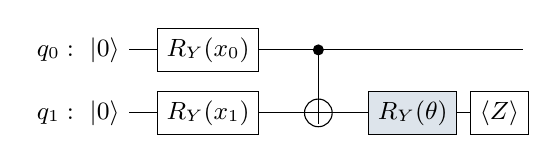
\begin{tikzpicture}[x=1cm, y=0.8cm, font=\small]
\draw (0,0) node[left]{$q_0:\ \ket0$} -- (5,0); \draw (0,-1) node[left]{$q_1:\ \ket0$} -- (5,-1);
\node[draw, fill=white] at (1,0) {$R_Y(x_0)$}; \node[draw, fill=white] at (1,-1) {$R_Y(x_1)$};
\fill (2.4,0) circle (2pt); \draw (2.4,0) -- (2.4,-1.18); \draw (2.4,-1) circle (5pt);
\node[draw, fill=brand!15] at (3.6,-1) {$R_Y(\theta)$}; \node[draw, fill=white] at (4.7,-1) {$\langle Z\rangle$};
\end{tikzpicture}
\end{center}
\end{passagebox}
\needspace{13\baselineskip}
\begin{qitem}{59}
\qmeta{Paragraph based}{VQC output (Heisenberg picture)}
The model output $f(\mathbf x; \theta) = \langle Z_1\rangle$ equals
\par\smallskip\noindent\begin{tabularx}{\linewidth}{@{}*{2}{L}@{}}
\optlabel{A}\,$\cos\theta\cos x_1 - \sin\theta\sin x_0\sin x_1$ & \correctlabel{B}\,$\cos\theta\cos x_0\cos x_1 - \sin\theta\sin x_1$ \\[3pt]
\optlabel{C}\,$\cos\theta\cos x_0\cos x_1 + \sin\theta\sin x_1$ & \optlabel{D}\,$\cos(\theta + x_1)\cos x_0$
\end{tabularx}
\end{qitem}
\begin{solbox}{B}
\textbf{\color{brand}Correct answer.} \textcolor{okgreen}{\textbf{(B)}} $\cos\theta\cos x_0\cos x_1 - \sin\theta\sin x_1$

\textbf{\color{brand}Concepts required.} Heisenberg picture for a small VQC; CNOT propagation rules.

\textbf{\color{brand}Relevant formulae.} $R_Y^\dagger ZR_Y = \cos\theta Z - \sin\theta X$; CNOT: $Z_t \to Z_cZ_t$, $X_t \to X_t$; $\langle X\rangle = \sin x$ for $R_Y(x)\ket0$.

\textbf{\color{brand}Step-by-step explanation.} Work backwards with the observable (Heisenberg picture). (1) Through $R_Y(\theta)$ on qubit 1:
$Z_1 \to \cos\theta\,Z_1 - \sin\theta\,X_1$ (from $R_Y^\dagger ZR_Y = \cos\theta Z - \sin\theta X$). (2) Through the CNOT: $Z$ on the target
becomes $Z_0Z_1$, while $X$ on the target is unchanged. (3) On the product state $R_Y(x_0)\ket0\otimes R_Y(x_1)\ket0$:
$\langle Z_0\rangle = \cos x_0$, $\langle Z_1\rangle = \cos x_1$, $\langle X_1\rangle = \sin x_1$.
Hence $f = \cos\theta\cos x_0\cos x_1 - \sin\theta\sin x_1$.

\textbf{\color{brand}Why the other options are incorrect.}
\begin{itemize}[leftmargin=2.4em, itemsep=1pt, topsep=2pt]
\item[\textbf{(A)}] This attaches $\cos x_0$ to the wrong term and turns $\langle X_1\rangle$ into $\sin x_0\sin x_1$.
\item[\textbf{(C)}] $+\sin\theta\sin x_1$ has the sign of the conjugation wrong.
\item[\textbf{(D)}] $\cos(\theta + x_1)\cos x_0$ attaches $\cos x_0$ to the $X_1$ term too; $X$ on the target does not pick up $Z_0$.
\end{itemize}
\textbf{\color{brand}Key takeaway.} Push the observable back through the gates, then evaluate on the product state.
\end{solbox}
\qsep

\needspace{13\baselineskip}
\begin{qitem}{60}
\qmeta{Paragraph based}{VQC gradient by parameter shift}
For $\mathbf x = (0, \frac\pi3)$, $\theta = \frac\pi6$ and label $y = +1$, the shifted outputs $f(\theta + \frac\pi2)$, $f(\theta - \frac\pi2)$ and
the loss gradient $\partial L/\partial\theta$ are
\par\smallskip\noindent\begin{tabularx}{\linewidth}{@{}*{4}{L}@{}}
\optlabel{A}\,$+1,\ -1,\ +2$ & \optlabel{B}\,$-1,\ +1,\ -2$ & \optlabel{C}\,$-1,\ +1,\ -1$ & \correctlabel{D}\,$-1,\ +1,\ +2$
\end{tabularx}
\end{qitem}
\begin{solbox}{D}
\textbf{\color{brand}Correct answer.} \textcolor{okgreen}{\textbf{(D)}} $-1,\ +1,\ +2$

\textbf{\color{brand}Concepts required.} Parameter shift + chain rule = gradient of the training loss.

\textbf{\color{brand}Relevant formulae.} $f' = \frac12[f(\theta + \frac\pi2) - f(\theta - \frac\pi2)]$; $\frac{\partial L}{\partial\theta} = 2(f - y)f'$.

\textbf{\color{brand}Step-by-step explanation.} With $x_0 = 0$, $x_1 = \frac\pi3$: $f(\theta) = \frac12\cos\theta - \frac{\sqrt3}{2}\sin\theta = \cos(\theta + \frac\pi3)$.
$f(\frac\pi6) = \cos\frac\pi2 = 0$; $f(\frac\pi6 + \frac\pi2) = f(\frac{2\pi}3) = \cos(\frac{2\pi}3 + \frac\pi3) = \cos\pi = -1$;
$f(\frac\pi6 - \frac\pi2) = f(-\frac\pi3) = \cos(-\frac\pi3 + \frac\pi3) = 1$.
Parameter shift: $f'(\theta) = \frac12(-1 - 1) = -1$ (exact; check $f' = -\sin(\theta + \frac\pi3) = -1$).
Chain rule: $\frac{\partial L}{\partial\theta} = 2(f - y)f' = 2(0 - 1)(-1) = +2$. A gradient step $\theta \leftarrow \theta - \eta\cdot2$ decreases $\theta$,
which increases $f$ towards the label $+1$.

\textbf{\color{brand}Why the other options are incorrect.}
\begin{itemize}[leftmargin=2.4em, itemsep=1pt, topsep=2pt]
\item[\textbf{(A)}] The shifted values are swapped: $f(\frac{2\pi}{3}) = \cos\pi = -1$, $f(-\frac\pi3) = \cos0 = +1$.
\item[\textbf{(B)}] $-2$ has the sign of $\partial L/\partial\theta$ wrong: $2(f - y)f' = 2(-1)(-1) = +2$.
\item[\textbf{(C)}] $-1$ is $f'(\theta)$, the derivative of the \emph{output}, not of the loss.
\end{itemize}
\textbf{\color{brand}Key takeaway.} Quantum part: $f'$ by parameter shift; classical part: chain rule through the loss.
\end{solbox}
\qsep

\newpage

\begin{sectionbanner}SECTION D \enspace$\cdot$\enspace Advanced QML and Implementation \hfill Q.61--80\end{sectionbanner}

\needspace{13\baselineskip}
\begin{qitem}{61}
\qmeta{Single-correct MCQ}{Barren plateau: shots needed}
For a deep random circuit with a global cost function the gradient components satisfy $\mathbb E[\partial_kC] = 0$ and
$\operatorname{Var}[\partial_kC] \approx 2^{-n}$. Each cost value is estimated with $S$ shots (statistical error $\approx 1/\sqrt S$). To resolve a
typical gradient component at $n = 20$ qubits one needs roughly
\par\smallskip\noindent\begin{tabularx}{\linewidth}{@{}*{4}{L}@{}}
\optlabel{A}\,$S \sim 20$ shots & \correctlabel{B}\,$S \sim 10^{6}$ shots & \optlabel{C}\,$S \sim 10^{12}$ shots & \optlabel{D}\,$S \sim 400$ shots
\end{tabularx}
\end{qitem}
\begin{solbox}{B}
\textbf{\color{brand}Correct answer.} \textcolor{okgreen}{\textbf{(B)}} $S \sim 10^{6}$ shots

\textbf{\color{brand}Concepts required.} Barren plateaus make gradients exponentially small; estimating them needs exponentially many shots.

\textbf{\color{brand}Relevant formulae.} $\operatorname{Var}[\partial_kC] \sim 2^{-n}$; shot error $\sim 1/\sqrt S$; need $1/\sqrt S \lesssim 2^{-n/2}$.

\textbf{\color{brand}Step-by-step explanation.} A typical gradient has size $\sqrt{\operatorname{Var}} = 2^{-n/2}$ (by Chebyshev, $|\partial_kC| \ge \epsilon$ has probability $\le 2^{-n}/\epsilon^2$).
To see it above the shot noise we need $1/\sqrt S \lesssim 2^{-n/2}$, i.e.\ $S \gtrsim 2^n = 2^{20} \approx 1.05\times10^6$ ---
\emph{exponentially} many shots in the number of qubits: a barren plateau. Comparing the noise with the variance instead of the
standard deviation would give $2^{2n} \approx 10^{12}$; polynomial guesses ($n$, $n^2$) miss the exponential scaling.

\textbf{\color{brand}Why the other options are incorrect.}
\begin{itemize}[leftmargin=2.4em, itemsep=1pt, topsep=2pt]
\item[\textbf{(A)}] $20$ shots ($= n$) assumes polynomial scaling, ignoring the $2^{-n}$ variance.
\item[\textbf{(C)}] $10^{12} = 2^{2n}$ compares the shot error with the variance instead of the standard deviation.
\item[\textbf{(D)}] $400 = n^2$ is also polynomial; it misses the exponential.
\end{itemize}
\textbf{\color{brand}Key takeaway.} Shots $\sim 2^n$: at 20 qubits about a million per gradient component.
\end{solbox}
\qsep

\needspace{13\baselineskip}
\begin{qitem}{62}
\qmeta{Single-correct MCQ}{Barren plateaus: what is known}
Which statement about barren plateaus is correct?
\begin{itemize}[leftmargin=2.6em, labelsep=0.4em, itemsep=2pt, topsep=3pt]
\item[\correctlabel{A}] For random circuits deep enough to form approximate 2-designs, gradient variances vanish exponentially in $n$; for shallow circuits, local cost functions have only polynomially vanishing gradients while global cost functions can still vanish exponentially.
\item[\optlabel{B}] Barren plateaus are caused only by hardware noise, so they never appear in noiseless simulation.
\item[\optlabel{C}] Switching to a gradient-free optimizer such as COBYLA removes a barren plateau, because no gradients are computed.
\item[\optlabel{D}] A barren plateau can be removed by multiplying the learning rate by $2^n$.
\end{itemize}
\end{qitem}
\begin{solbox}{A}
\textbf{\color{brand}Correct answer.} \textcolor{okgreen}{\textbf{(A)}} For random circuits deep enough to form approximate 2-designs, gradient variances vanish exponentially in $n$; for shallow circuits, local cost functions have only polynomially vanishing gradients while global cost functions can still vanish exponentially.

\textbf{\color{brand}Concepts required.} Known results about barren plateaus: depth, cost locality, noise, optimizer independence.

\textbf{\color{brand}Relevant formulae.} 2-design: $\operatorname{Var}[\partial C] \in O(2^{-n})$; shallow + local cost: $\Omega(1/\mathrm{poly}(n))$; global cost: $O(2^{-n})$.

\textbf{\color{brand}Step-by-step explanation.} McClean et al.\ (2018) showed exponentially vanishing gradient variance for random parameterised circuits that approximate
2-designs; Cerezo et al.\ (2021) showed that for shallow (logarithmic-depth) circuits the \emph{locality} of the cost matters: local costs
give polynomially vanishing gradients, global ones (e.g.\ fidelity with a target state) exponentially vanishing ones.
Noise can \emph{cause} additional plateaus (Wang et al.\ 2021), but noiseless deep circuits already have them. A flat landscape is flat for
every optimizer: cost \emph{differences} are exponentially small too (Arrasmith et al.\ 2021). Rescaling the step does not help because
the gradient estimate is dominated by shot noise.

\textbf{\color{brand}Why the other options are incorrect.}
\begin{itemize}[leftmargin=2.4em, itemsep=1pt, topsep=2pt]
\item[\textbf{(B)}] Noiseless random circuits already have barren plateaus (McClean et al.); noise adds further ones.
\item[\textbf{(C)}] Gradient-free optimizers also need cost differences, which are exponentially small on a plateau.
\item[\textbf{(D)}] The gradient \emph{estimate} is shot-noise dominated; scaling the step amplifies the noise too.
\end{itemize}
\textbf{\color{brand}Key takeaway.} Avoid plateaus by structure: shallow circuits, local costs, symmetric architectures (e.g.\ QCNN), smart initialisation.
\end{solbox}
\qsep

\needspace{13\baselineskip}
\begin{qitem}{63}
\qmeta{Single-correct MCQ}{Two- vs.\ four-term shift rule}
In a Hadamard test with a controlled-$R_Z(\theta)$ the measured output is $f(\theta) = \cos(\theta/2)$ (a pure frequency
$\frac12$). At $\theta = \pi$, the two-term shift formula $\frac12[f(\theta + \frac\pi2) - f(\theta - \frac\pi2)]$ and the exact derivative $f'(\pi)$ are
\par\smallskip\noindent\begin{tabularx}{\linewidth}{@{}*{2}{L}@{}}
\correctlabel{A}\,$-0.707$ and $-0.5$ & \optlabel{B}\,$-0.5$ and $-0.5$ \\[3pt]
\optlabel{C}\,$-1$ and $-0.5$ & \optlabel{D}\,$-0.707$ and $-0.707$
\end{tabularx}
\end{qitem}
\begin{solbox}{A}
\textbf{\color{brand}Correct answer.} \textcolor{okgreen}{\textbf{(A)}} $-0.707$ and $-0.5$

\textbf{\color{brand}Concepts required.} Generalised parameter-shift rules for generators with more than two eigenvalues.

\textbf{\color{brand}Relevant formulae.} Two-term: exact for frequency 1; four-term: $d_\pm = \frac{\sqrt2 \pm 1}{4\sqrt2}$, shifts $\frac\pi2$ and $\frac{3\pi}2$.

\textbf{\color{brand}Step-by-step explanation.} Exact: $f'(\theta) = -\frac12\sin\frac\theta2$, so $f'(\pi) = -\frac12$.
Two-term formula: $\frac12[\cos\frac{3\pi}{4} - \cos\frac\pi4] = \frac12\big[-\frac{\sqrt2}{2} - \frac{\sqrt2}{2}\big] = -\frac{\sqrt2}{2} \approx -0.707$ --- wrong
by $41\,\%$. The two-term rule is exact only when the generator has two eigenvalues $\pm\frac12$ (frequency 1). A controlled rotation has
eigenvalues $0, \pm\frac12$ (frequencies $\frac12$ and $1$); the four-term rule
$f' = d_+[f(\theta + \frac\pi2) - f(\theta - \frac\pi2)] - d_-[f(\theta + \frac{3\pi}2) - f(\theta - \frac{3\pi}2)]$, $d_\pm = \frac{\sqrt2 \pm 1}{4\sqrt2}$,
gives exactly $-0.5$.

\textbf{\color{brand}Why the other options are incorrect.}
\begin{itemize}[leftmargin=2.4em, itemsep=1pt, topsep=2pt]
\item[\textbf{(B)}] $-0.5$ for the two-term formula assumes it is exact; it is not for frequency $\frac12$.
\item[\textbf{(C)}] $-1$ omits the factor $\frac12$ of the shift formula.
\item[\textbf{(D)}] $-0.707$ is not the exact derivative; $\frac{d}{d\theta}\cos\frac\theta2 = -\frac12\sin\frac\theta2 = -\frac12$ at $\pi$.
\end{itemize}
\textbf{\color{brand}Key takeaway.} Controlled rotations need the four-term rule; the naive two-term rule is biased.
\end{solbox}
\qsep

\needspace{13\baselineskip}
\begin{qitem}{64}
\qmeta{Single-correct MCQ}{Depolarising noise and accuracy}
In a simple global-depolarising model every gate multiplies the output expectation value by $(1 - p)$. For the default
QCNN (69 gates) and $p = 0.01$, the expectation values are multiplied by about ..., and the test \emph{accuracy} (prediction
$\operatorname{sign}\langle Z\rangle$) is expected to
\begin{itemize}[leftmargin=2.6em, labelsep=0.4em, itemsep=2pt, topsep=3pt]
\item[\optlabel{A}] $0.31$; drop to $50\,\%$
\item[\correctlabel{B}] $0.50$; stay the same, while $|\langle Z\rangle|$ shrinks and the MSE grows
\item[\optlabel{C}] $0.50$; drop to about $50\,\%$, because half of the predictions flip sign
\item[\optlabel{D}] $0.99$; stay the same, and noise is negligible
\end{itemize}
\end{qitem}
\begin{solbox}{B}
\textbf{\color{brand}Correct answer.} \textcolor{okgreen}{\textbf{(B)}} $0.50$; stay the same, while $|\langle Z\rangle|$ shrinks and the MSE grows

\textbf{\color{brand}Concepts required.} Depolarising noise shrinks expectation values towards 0 without (on average) flipping their sign.

\textbf{\color{brand}Relevant formulae.} $\langle Z\rangle_{\text{noisy}} \approx (1 - p)^G\langle Z\rangle$; $(1 - p)^G \approx e^{-pG}$ for small $p$.

\textbf{\color{brand}Step-by-step explanation.} $(1 - 0.01)^{69} = e^{69\ln0.99} = e^{-0.6935} \approx 0.50$. Multiplying every output by a positive factor does not change its
sign, so sign-based accuracy is unchanged in this model; but the outputs move towards 0, so the MSE $\frac1M\sum(f - y)^2$ grows
towards 1 and, with finite shots, small outputs become indistinguishable from 0. (The lecture's density-matrix simulation with
gate-level depolarising noise $p = 0.01$ found exactly this: accuracy stayed $85\,\%$ while the mean $|\langle Z\rangle|$ fell from $0.171$ to $0.112$.)

\textbf{\color{brand}Why the other options are incorrect.}
\begin{itemize}[leftmargin=2.4em, itemsep=1pt, topsep=2pt]
\item[\textbf{(A)}] $0.31$ uses $e^{-pG}$ with the wrong exponent; and a positive scale factor cannot flip signs.
\item[\textbf{(C)}] A common positive factor keeps every sign; accuracy does not collapse in this model.
\item[\textbf{(D)}] $0.99$ is one gate's factor; 69 gates compound to about $0.5$.
\end{itemize}
\textbf{\color{brand}Key takeaway.} Noise shrinks margins (and raises MSE) before it flips predictions; small margins are fragile.
\end{solbox}
\qsep

\needspace{13\baselineskip}
\begin{qitem}{65}
\qmeta{Single-correct MCQ}{GPU memory and multi-GPU qubits}
An 80 GB GPU simulates state vectors in double precision (16 bytes per amplitude). The largest number of qubits that
fits on one GPU, and on four such GPUs pooled for one distributed state vector, are
\par\smallskip\noindent\begin{tabularx}{\linewidth}{@{}*{4}{L}@{}}
\optlabel{A}\,$36$ and $38$ & \optlabel{B}\,$32$ and $128$ & \optlabel{C}\,$33$ and $35$ & \correctlabel{D}\,$32$ and $34$
\end{tabularx}
\end{qitem}
\begin{solbox}{D}
\textbf{\color{brand}Correct answer.} \textcolor{okgreen}{\textbf{(D)}} $32$ and $34$

\textbf{\color{brand}Concepts required.} GPU memory limits of state-vector simulation; distributed (multi-GPU) state vectors.

\textbf{\color{brand}Relevant formulae.} $n_{\max} = \lfloor\log_2(\text{memory}/b)\rfloor$, $b = 16$ (fp64) or $8$ (fp32).

\textbf{\color{brand}Step-by-step explanation.} Need $16\cdot2^n \le 80\times10^9$: $2^{32}\cdot16 = 68.7$ GB fits, $2^{33}\cdot16 = 137$ GB does not, so $n = 32$.
Four GPUs give 320 GB: $2^{34}\cdot16 = 275$ GB fits, $2^{35}\cdot16 = 550$ GB does not, so $n = 34$. Multiplying the memory by 4
adds only $\log_2 4 = 2$ qubits. (In single precision, 8 bytes, the answers would be 33 and 35.)

\textbf{\color{brand}Why the other options are incorrect.}
\begin{itemize}[leftmargin=2.4em, itemsep=1pt, topsep=2pt]
\item[\textbf{(A)}] $36$ and $38$ divide bytes as if they were bits.
\item[\textbf{(B)}] $128$ scales qubits linearly with memory; memory scales as $2^n$.
\item[\textbf{(C)}] $33$ and $35$ are the single-precision (8-byte) answers.
\end{itemize}
\textbf{\color{brand}Key takeaway.} $4\times$ the memory buys only 2 more qubits.
\end{solbox}
\qsep

\needspace{13\baselineskip}
\begin{qitem}{66}
\qmeta{Single-correct MCQ}{Cost of an exact QCNN gradient}
Suppose the 8-qubit QCNN (11 convolution blocks, 7 pooling blocks) were trained by gradient descent with \emph{exact}
parameter-shift gradients: every $R_Y$ occurrence shifted separately (2 circuits), every controlled rotation (\texttt{crz}, \texttt{crx})
with the four-term rule (4 circuits). The number of circuits for \emph{one} full gradient of the loss over the 20 training images is
\par\smallskip\noindent\begin{tabularx}{\linewidth}{@{}*{4}{L}@{}}
\optlabel{A}\,$480$ & \optlabel{B}\,$1440$ & \optlabel{C}\,$40$ & \correctlabel{D}\,$2000$
\end{tabularx}
\end{qitem}
\begin{solbox}{D}
\textbf{\color{brand}Correct answer.} \textcolor{okgreen}{\textbf{(D)}} $2000$

\textbf{\color{brand}Concepts required.} Cost of exact gradients for circuits with shared parameters and controlled rotations.

\textbf{\color{brand}Relevant formulae.} Per image: $\sum_{\text{conv}}2\times2 + \sum_{\text{pool}}2\times4 = 4n_{\text{conv}} + 8n_{\text{pool}}$.

\textbf{\color{brand}Step-by-step explanation.} Per image: each convolution block has 2 $R_Y$ gates $\Rightarrow 2\times2 = 4$ circuits per block, $11\times4 = 44$; each pooling block has one
\texttt{crz} and one \texttt{crx} $\Rightarrow 2\times4 = 8$ circuits per block, $7\times8 = 56$. Total $44 + 56 = 100$ circuits per image, and
$100\times20 = 2000$ for the training set (plus the 20 forward passes for the loss). One exact gradient step costs as much as the
\emph{whole} 100-evaluation COBYLA run of the notebook. (480 = naive $2\times12\times20$; 1440 = two-term rule for every occurrence.)

\textbf{\color{brand}Why the other options are incorrect.}
\begin{itemize}[leftmargin=2.4em, itemsep=1pt, topsep=2pt]
\item[\textbf{(A)}] $480 = 2\times12\times20$ shifts each shared parameter once with the two-term rule: wrong for shared and controlled gates.
\item[\textbf{(B)}] $1440$ shifts every occurrence but uses the two-term rule for the controlled rotations, which is not exact.
\item[\textbf{(C)}] $40$ counts two circuits per image only.
\end{itemize}
\textbf{\color{brand}Key takeaway.} Exact gradients are expensive: one step costs as much as the whole COBYLA run here.
\end{solbox}
\qsep

\needspace{13\baselineskip}
\begin{qitem}{67}
\qmeta{Single-correct MCQ}{Expectation values from counts}
\texttt{cudaq.sample} on a two-qubit kernel returns the counts \texttt{\{'00': 400, '01': 100, '10': 300, '11': 200\}}
(the first character is qubit 0). The estimates of $\big(\langle Z_0\rangle, \langle Z_1\rangle, \langle Z_0Z_1\rangle\big)$ are
\par\smallskip\noindent\begin{tabularx}{\linewidth}{@{}*{4}{L}@{}}
\correctlabel{A}\,$(0,\ 0.4,\ 0.2)$ & \optlabel{B}\,$(0,\ 0.4,\ 0)$ & \optlabel{C}\,$(0,\ 0.4,\ 0.6)$ & \optlabel{D}\,$(0.4,\ 0,\ 0.2)$
\end{tabularx}
\end{qitem}
\begin{solbox}{A}
\textbf{\color{brand}Correct answer.} \textcolor{okgreen}{\textbf{(A)}} $(0,\ 0.4,\ 0.2)$

\textbf{\color{brand}Concepts required.} Estimating Pauli expectation values from bitstring counts; CUDA-Q writes qubit 0 first.

\textbf{\color{brand}Relevant formulae.} $\langle Z_i\rangle = \sum_sp_s(-1)^{s_i}$, $\langle Z_0Z_1\rangle = \sum_sp_s(-1)^{s_0 + s_1}$.

\textbf{\color{brand}Step-by-step explanation.} Total 1000 shots. Qubit 0 is $0$ in \texttt{00}, \texttt{01}: $P = 0.5$, so $\langle Z_0\rangle = 0.5 - 0.5 = 0$.
Qubit 1 is $0$ in \texttt{00}, \texttt{10}: $P = 0.7$, so $\langle Z_1\rangle = 0.7 - 0.3 = 0.4$.
$Z_0Z_1 = +1$ for even parity (\texttt{00}, \texttt{11}: 600) and $-1$ for odd parity (400): $\langle Z_0Z_1\rangle = 0.2$, which differs from
$\langle Z_0\rangle\langle Z_1\rangle = 0$, so the qubits are correlated. \texttt{cudaq.observe} computes such expectation values directly
(exactly on a state-vector simulator, or from shots with \texttt{shots\_count}).

\textbf{\color{brand}Why the other options are incorrect.}
\begin{itemize}[leftmargin=2.4em, itemsep=1pt, topsep=2pt]
\item[\textbf{(B)}] $\langle Z_0Z_1\rangle = 0$ multiplies the marginals; the parity counts give $0.2$.
\item[\textbf{(C)}] $0.6$ is $P(\text{even parity})$, not $P(\text{even}) - P(\text{odd})$.
\item[\textbf{(D)}] $(0.4, 0)$ reads the bitstrings in the wrong order (last character = qubit 0).
\end{itemize}
\textbf{\color{brand}Key takeaway.} Marginalise the counts per qubit; parity gives correlators.
\end{solbox}
\qsep

\needspace{13\baselineskip}
\begin{qitem}{68}
\qmeta{Single-correct MCQ}{Interpreting MSE 0.67 at 90\,\% accuracy}
The recorded run of \texttt{QML.ipynb} ends with training accuracy $90\,\%$ but training MSE $0.67$ (the mean
$|\langle Z_7\rangle|$ of the trained model on the training images is about $0.20$). The best explanation is
\begin{itemize}[leftmargin=2.6em, labelsep=0.4em, itemsep=2pt, topsep=3pt]
\item[\correctlabel{A}] the outputs have the correct sign but small magnitude, so each correct image still contributes about $(1 - 0.2)^2 = 0.64$ to the loss
\item[\optlabel{B}] a bug: for $\pm1$ labels the MSE must equal $1 - \text{accuracy} = 0.10$
\item[\optlabel{C}] COBYLA diverged in the last iterations, so the loss and the accuracy belong to different parameter vectors
\item[\optlabel{D}] the MSE is computed on the test images, the accuracy on the training images
\end{itemize}
\end{qitem}
\begin{solbox}{A}
\textbf{\color{brand}Correct answer.} \textcolor{okgreen}{\textbf{(A)}} the outputs have the correct sign but small magnitude, so each correct image still contributes about $(1 - 0.2)^2 = 0.64$ to the loss

\textbf{\color{brand}Concepts required.} MSE vs.\ accuracy; output margins of a trained QCNN.

\textbf{\color{brand}Relevant formulae.} For a correct prediction with $|f| = m$: $(f - y)^2 = (1 - m)^2$.

\textbf{\color{brand}Step-by-step explanation.} MSE measures the distance of the real-valued output from $\pm1$; accuracy only checks the sign. If $\langle Z\rangle = \pm0.2$ with the
right sign, the squared error is $(1 - 0.2)^2 = 0.64$ even though the prediction is correct. A mean $|\langle Z\rangle|$ of $0.2$ is
consistent with an MSE of $0.67$ and $90\,\%$ accuracy. The notebook prints both quantities for the same final parameters on the
training set. Small margins matter: with few shots or noise such predictions are fragile.

\textbf{\color{brand}Why the other options are incorrect.}
\begin{itemize}[leftmargin=2.4em, itemsep=1pt, topsep=2pt]
\item[\textbf{(B)}] For outputs in $[-1, 1]$ there is no identity $\text{MSE} = 1 - \text{accuracy}$; that would hold only for outputs exactly $\pm1$ (then MSE $= 4(1 - \text{acc})$).
\item[\textbf{(C)}] COBYLA returns its best point; the notebook recomputes the loss and accuracy at the same final parameters.
\item[\textbf{(D)}] Both are computed on the training set (the test MSE is not printed).
\end{itemize}
\textbf{\color{brand}Key takeaway.} High accuracy with high MSE means correct but low-confidence outputs.
\end{solbox}
\qsep

\needspace{13\baselineskip}
\begin{qitem}{69}
\qmeta{Single-correct MCQ}{15-qubit training time}
The README of the repository reports a 15-qubit test of \texttt{QML.ipynb} ($3\times5$ images, 16 training images, 60 COBYLA
evaluations) at about $0.35$ s per circuit on the 4-core test CPU. The training time is about
\par\smallskip\noindent\begin{tabularx}{\linewidth}{@{}*{4}{L}@{}}
\optlabel{A}\,$21$ seconds & \correctlabel{B}\,$5.6$ minutes & \optlabel{C}\,$0.35$ seconds & \optlabel{D}\,$56$ minutes
\end{tabularx}
\end{qitem}
\begin{solbox}{B}
\textbf{\color{brand}Correct answer.} \textcolor{okgreen}{\textbf{(B)}} $5.6$ minutes

\textbf{\color{brand}Concepts required.} Training cost = evaluations $\times$ images $\times$ time per circuit.

\textbf{\color{brand}Relevant formulae.} $T \approx n_{\text{eval}}\cdot M\cdot t_{\text{circuit}}$.

\textbf{\color{brand}Step-by-step explanation.} Circuits $= 60$ evaluations $\times$ 16 images $= 960$; time $\approx 960\times0.35\ \text{s} = 336\ \text{s} \approx 5.6$ minutes.
(Compare 8 qubits: $1.7$ ms per circuit. Going from 8 to 15 qubits multiplies the state size by $2^7 = 128$ and the gate count from
69 to 146, so a factor of about 200 is expected.) This is why the notebook recommends a GPU for 15 or more qubits.

\textbf{\color{brand}Why the other options are incorrect.}
\begin{itemize}[leftmargin=2.4em, itemsep=1pt, topsep=2pt]
\item[\textbf{(A)}] $21$ s forgets the 16 images per evaluation.
\item[\textbf{(C)}] $0.35$ s is the time of one circuit.
\item[\textbf{(D)}] $56$ min is ten times too large.
\end{itemize}
\textbf{\color{brand}Key takeaway.} $60\times16\times0.35$ s $\approx 5.6$ min on a CPU: GPU recommended beyond $\sim15$ qubits.
\end{solbox}
\qsep

\needspace{13\baselineskip}
\begin{qitem}{70}
\qmeta{Single-correct MCQ}{Kernel concentration}
For the product kernel $k(\mathbf x, \mathbf x') = \prod_{i=1}^{n}\cos^2\frac{\pi(x_i - x'_i)}{2}$ with all $x_i, x'_i$ independent
and uniform on $[0, 1]$, the average off-diagonal kernel value $\mathbb E[k]$ equals
\par\smallskip\noindent\begin{tabularx}{\linewidth}{@{}*{2}{L}@{}}
\optlabel{A}\,$(2/\pi)^n$ & \optlabel{B}\,$2^{-n}$ \\[3pt]
\correctlabel{C}\,$\big(\tfrac12 + \tfrac{2}{\pi^2}\big)^n \approx 0.70^n$ & \optlabel{D}\,$1/n$
\end{tabularx}
\end{qitem}
\begin{solbox}{C}
\textbf{\color{brand}Correct answer.} \textcolor{okgreen}{\textbf{(C)}} $\big(\tfrac12 + \tfrac{2}{\pi^2}\big)^n \approx 0.70^n$

\textbf{\color{brand}Concepts required.} Exponential concentration of kernel values for product feature maps with many features.

\textbf{\color{brand}Relevant formulae.} $\mathbb E[k] = \prod_i\mathbb E\cos^2\frac{\pi\Delta_i}2$; $\mathbb E\cos\pi(x - x') = |\mathbb Ee^{i\pi x}|^2 = 4/\pi^2$.

\textbf{\color{brand}Step-by-step explanation.} Independence factorises the expectation: $\mathbb E[k] = \big(\mathbb E\cos^2\frac{\pi\Delta}{2}\big)^n$, $\Delta = x - x'$.
$\cos^2\frac{\pi\Delta}{2} = \frac12 + \frac12\cos\pi\Delta$ and $\mathbb E\cos\pi(x - x') = |\mathbb E\,e^{i\pi x}|^2 = \big|\int_0^1e^{i\pi x}dx\big|^2 = \big|\frac{e^{i\pi} - 1}{i\pi}\big|^2 = \frac{4}{\pi^2}$.
So each factor is $\frac12 + \frac{2}{\pi^2} \approx 0.703$ and $\mathbb E[k] \approx 0.703^n$: kernel values \emph{concentrate} exponentially
towards 0 as the number of features grows ($0.703^{8} \approx 0.06$, $0.703^{50} \approx 2\times10^{-8}$), so exponentially many shots would
be needed to estimate them --- the exponential-concentration problem of quantum kernels.

\textbf{\color{brand}Why the other options are incorrect.}
\begin{itemize}[leftmargin=2.4em, itemsep=1pt, topsep=2pt]
\item[\textbf{(A)}] $(2/\pi)^n$ uses $|\mathbb Ee^{i\pi x}|$ instead of $\frac12 + \frac12|\mathbb Ee^{i\pi x}|^2$.
\item[\textbf{(B)}] $2^{-n}$ assumes every factor averages $\frac12$, i.e.\ drops the term $\frac12\mathbb E\cos\pi\Delta = 2/\pi^2$.
\item[\textbf{(D)}] $1/n$ is polynomial; independent factors multiply, giving exponential decay.
\end{itemize}
\textbf{\color{brand}Key takeaway.} Product kernels concentrate like $c^n$ ($c \approx 0.70$ here): more features $\Rightarrow$ kernel values $\to 0$.
\end{solbox}
\qsep

\needspace{13\baselineskip}
\begin{qitem}{71}
\qmeta{Single-correct MCQ}{Quantum PCA}
Which statement about quantum principal component analysis (qPCA, Lloyd, Mohseni \& Rebentrost 2014) is correct?
\begin{itemize}[leftmargin=2.6em, labelsep=0.4em, itemsep=2pt, topsep=3pt]
\item[\correctlabel{A}] It uses many copies of a density matrix $\rho$ to apply $e^{-i\rho t}$ (density-matrix exponentiation) and phase estimation to reveal its large eigenvalues; the output is a quantum state, and any speed-up assumes efficient state preparation and low rank --- dequantized classical algorithms match it under comparable assumptions.
\item[\optlabel{B}] It is the pooling layer of the QCNN in \texttt{QML.ipynb}.
\item[\optlabel{C}] It diagonalises the covariance matrix of $N$ classical data points in $O(\log N)$ total time, including loading the data and reading out all eigenvectors.
\item[\optlabel{D}] It needs only a single copy of $\rho$, because one measurement reveals all eigenvalues.
\end{itemize}
\end{qitem}
\begin{solbox}{A}
\textbf{\color{brand}Correct answer.} \textcolor{okgreen}{\textbf{(A)}} It uses many copies of a density matrix $\rho$ to apply $e^{-i\rho t}$ (density-matrix exponentiation) and phase estimation to reveal its large eigenvalues; the output is a quantum state, and any speed-up assumes efficient state preparation and low rank --- dequantized classical algorithms match it under comparable assumptions.

\textbf{\color{brand}Concepts required.} What qPCA actually does, and its assumptions.

\textbf{\color{brand}Relevant formulae.} $e^{-i\rho t}$ from copies of $\rho$ (partial SWAPs); phase estimation gives $\lambda_k$ with $\ket{v_k}$; cost polylog only for low rank with efficient state access.

\textbf{\color{brand}Step-by-step explanation.} qPCA prepares many copies of $\rho$ (the normalised covariance/density matrix), simulates $e^{-i\rho t}$ by repeated partial SWAPs with
fresh copies, and runs phase estimation to obtain eigenvalue estimates together with the eigenvectors \emph{as quantum states}.
Reading out classical eigenvectors costs time proportional to their dimension, and loading classical data needs QRAM-like assumptions;
Tang-style ``dequantized'' sampling algorithms reach similar polylogarithmic scaling for low-rank matrices with comparable access. One copy
cannot reveal a spectrum (no-cloning, measurement collapse). qPCA is \emph{not} implemented in this repository.

\textbf{\color{brand}Why the other options are incorrect.}
\begin{itemize}[leftmargin=2.4em, itemsep=1pt, topsep=2pt]
\item[\textbf{(B)}] The QCNN pooling block is a controlled rotation; qPCA is not in the repository.
\item[\textbf{(C)}] Loading $N$ classical points and reading out eigenvectors each cost at least linear time; no end-to-end $O(\log N)$ is known.
\item[\textbf{(D)}] One copy of an unknown state cannot reveal its spectrum; qPCA consumes many copies.
\end{itemize}
\textbf{\color{brand}Key takeaway.} qPCA's speed-up lives in the assumptions (state access, low rank, quantum output).
\end{solbox}
\qsep

\needspace{13\baselineskip}
\begin{qitem}{72}
\qmeta{Single-correct MCQ}{GAN equilibrium}
A (quantum or classical) GAN optimises $V(D, G) = \mathbb E_{x\sim p_{\text{data}}}[\ln D(x)] + \mathbb E_{x\sim p_G}[\ln(1 - D(x))]$.
At the ideal equilibrium $p_G = p_{\text{data}}$ with the optimal discriminator, the value of $V$ is
\par\smallskip\noindent\begin{tabularx}{\linewidth}{@{}*{4}{L}@{}}
\optlabel{A}\,$0$ & \optlabel{B}\,$-\tfrac12$ & \correctlabel{C}\,$-\ln 4 \approx -1.386$ & \optlabel{D}\,$\ln 2$
\end{tabularx}
\end{qitem}
\begin{solbox}{C}
\textbf{\color{brand}Correct answer.} \textcolor{okgreen}{\textbf{(C)}} $-\ln 4 \approx -1.386$

\textbf{\color{brand}Concepts required.} GAN minimax objective and its equilibrium.

\textbf{\color{brand}Relevant formulae.} $D^* = \frac{p_{\text{data}}}{p_{\text{data}} + p_G}$; at $p_G = p_{\text{data}}$: $D^* = \frac12$, $V = 2\ln\frac12$.

\textbf{\color{brand}Step-by-step explanation.} For fixed $G$ the optimal discriminator is $D^*(x) = \frac{p_{\text{data}}(x)}{p_{\text{data}}(x) + p_G(x)}$. When $p_G = p_{\text{data}}$, $D^* = \frac12$
everywhere, so $V = \ln\frac12 + \ln\frac12 = -2\ln2 = -\ln4$. In a quantum GAN the generator is a parameterised circuit whose
measurement distribution plays the role of $p_G$; training alternates discriminator and generator updates (not implemented in this repository).

\textbf{\color{brand}Why the other options are incorrect.}
\begin{itemize}[leftmargin=2.4em, itemsep=1pt, topsep=2pt]
\item[\textbf{(A)}] $0$ would need $D = 1$ on data and $D = 0$ on fakes, i.e.\ a perfect discriminator, not equilibrium.
\item[\textbf{(B)}] $-\frac12$ has no derivation from $V$.
\item[\textbf{(D)}] $\ln2$ is positive; $V$ is a sum of logarithms of probabilities and is $\le 0$.
\end{itemize}
\textbf{\color{brand}Key takeaway.} Equilibrium: the discriminator outputs $\frac12$ everywhere, $V = -\ln4$.
\end{solbox}
\qsep

\needspace{13\baselineskip}
\begin{qitem}{73}
\qmeta{Single-correct MCQ}{Q-learning update}
In (quantum) reinforcement learning with Q-learning, $Q(s, a) \leftarrow Q(s, a) + \alpha\big[r + \gamma\max_{a'}Q(s', a') - Q(s, a)\big]$.
With $Q(s, a) = 2$, $\alpha = 0.5$, reward $r = 1$, discount $\gamma = 0.9$ and $\max_{a'}Q(s', a') = 4$, the updated value is
\par\smallskip\noindent\begin{tabularx}{\linewidth}{@{}*{4}{L}@{}}
\optlabel{A}\,$3.5$ & \optlabel{B}\,$2.6$ & \correctlabel{C}\,$3.3$ & \optlabel{D}\,$4.6$
\end{tabularx}
\end{qitem}
\begin{solbox}{C}
\textbf{\color{brand}Correct answer.} \textcolor{okgreen}{\textbf{(C)}} $3.3$

\textbf{\color{brand}Concepts required.} Temporal-difference (Q-learning) update.

\textbf{\color{brand}Relevant formulae.} $Q \leftarrow Q + \alpha(r + \gamma\max_{a'}Q' - Q)$.

\textbf{\color{brand}Step-by-step explanation.} Target $= r + \gamma\max Q' = 1 + 0.9\times4 = 4.6$; temporal-difference error $= 4.6 - 2 = 2.6$;
update $= 2 + 0.5\times2.6 = 3.3$. In quantum RL a variational circuit can represent the Q-function or the policy
$\pi(a\mid s) = |\braket{a|U(s; \boldsymbol\theta)|0}|^2$; the update rule itself is classical.

\textbf{\color{brand}Why the other options are incorrect.}
\begin{itemize}[leftmargin=2.4em, itemsep=1pt, topsep=2pt]
\item[\textbf{(A)}] $3.5$ ignores the discount ($\gamma = 1$).
\item[\textbf{(B)}] $2.6$ is the TD error, not the new $Q$.
\item[\textbf{(D)}] $4.6$ is the target $r + \gamma\max Q'$, not the updated value (it would need $\alpha = 1$).
\end{itemize}
\textbf{\color{brand}Key takeaway.} New $Q$ = old $Q$ + learning rate $\times$ TD error.
\end{solbox}
\qsep

\needspace{13\baselineskip}
\begin{qitem}{74}
\qmeta{Single-correct MCQ}{Swap-test distances (clustering)}
A quantum clustering algorithm estimates distances between normalised real data vectors $\mathbf a, \mathbf b$ with a swap test.
The ancilla gives $0$ with probability $0.9$, and $\mathbf a\cdot\mathbf b > 0$ is known. The Euclidean distance $\|\mathbf a - \mathbf b\|$ is about
\par\smallskip\noindent\begin{tabularx}{\linewidth}{@{}*{4}{L}@{}}
\optlabel{A}\,$0.21$ & \correctlabel{B}\,$0.46$ & \optlabel{C}\,$0.63$ & \optlabel{D}\,$0.89$
\end{tabularx}
\end{qitem}
\begin{solbox}{B}
\textbf{\color{brand}Correct answer.} \textcolor{okgreen}{\textbf{(B)}} $0.46$

\textbf{\color{brand}Concepts required.} Distances from overlaps; swap test estimates $|\braket{a|b}|^2$.

\textbf{\color{brand}Relevant formulae.} $|\mathbf a\cdot\mathbf b|^2 = 2P(0) - 1$; $\|\mathbf a - \mathbf b\|^2 = 2 - 2\mathbf a\cdot\mathbf b$ for unit vectors.

\textbf{\color{brand}Step-by-step explanation.} Swap test: $|\mathbf a\cdot\mathbf b|^2 = 2P(0) - 1 = 0.8$, so $\mathbf a\cdot\mathbf b = \sqrt{0.8} = 0.894$.
For unit vectors $\|\mathbf a - \mathbf b\|^2 = 2 - 2\,\mathbf a\cdot\mathbf b = 2 - 1.789 = 0.211$, hence $\|\mathbf a - \mathbf b\| = 0.46$.
(Using $0.8$ as the overlap gives $\sqrt{0.4} = 0.63$.) The swap test only gives $|\mathbf a\cdot\mathbf b|$; the sign must be known
or obtained otherwise (e.g.\ a Hadamard test).

\textbf{\color{brand}Why the other options are incorrect.}
\begin{itemize}[leftmargin=2.4em, itemsep=1pt, topsep=2pt]
\item[\textbf{(A)}] $0.21$ is the squared distance.
\item[\textbf{(C)}] $0.63$ uses $0.8$ (the squared overlap) as the overlap.
\item[\textbf{(D)}] $0.89$ is the overlap $\mathbf a\cdot\mathbf b$, not the distance.
\end{itemize}
\textbf{\color{brand}Key takeaway.} Overlap $\to$ distance: take the square root of $2P(0) - 1$ first.
\end{solbox}
\qsep

\needspace{13\baselineskip}
\begin{qitem}{75}
\qmeta{Matching lists}{CUDA-Q targets}
Match each CUDA-Q target (List-I) with its use (List-II).
\par\smallskip\noindent{\renewcommand{\arraystretch}{1.35}%
\begin{tabularx}{\linewidth}{@{}c>{\raggedright\arraybackslash}p{0.33\linewidth}@{\hspace{1.2em}}cL@{}}
\toprule
\multicolumn{2}{@{}l}{\textbf{List-I}} & \multicolumn{2}{l@{}}{\textbf{List-II}} \\ \midrule
\textbf{(P)} & \texttt{qpp-cpu} & \textbf{(1)} & one state vector distributed over several GPUs (one MPI rank per GPU) to simulate more qubits \\
\textbf{(Q)} & \texttt{nvidia} with option \texttt{mgpu} & \textbf{(2)} & several independent virtual QPUs (one per GPU) that run \emph{different} circuits in parallel, e.g.\ many images or shift terms \\
\textbf{(R)} & \texttt{nvidia} with option \texttt{mqpu} & \textbf{(3)} & CPU state-vector simulator; produced the recorded outputs of \texttt{QML.ipynb} \\
\textbf{(S)} & \texttt{density-matrix-cpu} & \textbf{(4)} & noisy simulation with a noise model; memory $16\cdot4^N$ bytes \\
\bottomrule
\end{tabularx}}
\par\smallskip\noindent\begin{tabularx}{\linewidth}{@{}*{2}{L}@{}}
\optlabel{A}\,P$\to$3, Q$\to$1, R$\to$4, S$\to$2 & \optlabel{B}\,P$\to$4, Q$\to$1, R$\to$2, S$\to$3 \\[3pt]
\correctlabel{C}\,P$\to$3, Q$\to$1, R$\to$2, S$\to$4 & \optlabel{D}\,P$\to$3, Q$\to$2, R$\to$1, S$\to$4
\end{tabularx}
\end{qitem}
\begin{solbox}{C}
\textbf{\color{brand}Correct answer.} \textcolor{okgreen}{\textbf{(C)}} P$\to$3, Q$\to$1, R$\to$2, S$\to$4

\textbf{\color{brand}Concepts required.} CUDA-Q simulation targets and their use in QML workloads.

\textbf{\color{brand}Relevant formulae.} State vector: $16\cdot2^N$ B (\texttt{qpp-cpu}, \texttt{nvidia}); distributed: $16\cdot2^N/G$ per GPU (\texttt{mgpu}); density matrix: $16\cdot4^N$ B.

\textbf{\color{brand}Step-by-step explanation.} \begin{itemize}\itemsep0pt
\item \texttt{qpp-cpu}: the default when no GPU is visible; the notebook's recorded run used it (\texttt{GPUs visible to CUDA-Q: 0}) (3).
\item \texttt{mgpu} pools the memory of several GPUs for \emph{one} large state vector; it needs \texttt{mpiexec} (1).
\item \texttt{mqpu} exposes each GPU as a separate QPU for asynchronous, parallel execution of many \emph{small} circuits --- the natural
choice for QML, where each training step evaluates one circuit per image (2).
\item \texttt{density-matrix-cpu} stores $\rho$ ($4^N$ entries) and applies noise channels (4).
\end{itemize}
Hence P$\to$3, Q$\to$1, R$\to$2, S$\to$4. \texttt{QML.ipynb} itself selects only \texttt{nvidia} or \texttt{qpp-cpu} (or a user-given name) and uses neither \texttt{mgpu} nor \texttt{mqpu}.

\textbf{\color{brand}Why the other options are incorrect.}
\begin{itemize}[leftmargin=2.4em, itemsep=1pt, topsep=2pt]
\item[\textbf{(A)}] R$\to$4, S$\to$2: \texttt{mqpu} is a parallel noiseless state-vector mode; noise needs a density-matrix or trajectory target.
\item[\textbf{(B)}] P$\to$4, S$\to$3 swaps the CPU state-vector and density-matrix simulators.
\item[\textbf{(D)}] Q$\to$2, R$\to$1 swaps \texttt{mgpu} (one big state) and \texttt{mqpu} (many small circuits in parallel).
\end{itemize}
\textbf{\color{brand}Key takeaway.} QML batches many small circuits: \texttt{mqpu} parallelises them; \texttt{mgpu} only helps for very wide circuits.
\end{solbox}
\qsep

\needspace{13\baselineskip}
\begin{qitem}{76}
\qmeta{Matching lists}{Limitations of QML}
Match each limitation of QML (List-I) with its description (List-II).
\par\smallskip\noindent{\renewcommand{\arraystretch}{1.35}%
\begin{tabularx}{\linewidth}{@{}c>{\raggedright\arraybackslash}p{0.33\linewidth}@{\hspace{1.2em}}cL@{}}
\toprule
\multicolumn{2}{@{}l}{\textbf{List-I}} & \multicolumn{2}{l@{}}{\textbf{List-II}} \\ \midrule
\textbf{(P)} & barren plateau & \textbf{(1)} & classical sampling algorithms reproduce claimed exponential speed-ups (e.g.\ recommendation systems, PCA) under the same input assumptions \\
\textbf{(Q)} & dequantization & \textbf{(2)} & the variance of cost gradients decays exponentially with the number of qubits \\
\textbf{(R)} & data-loading bottleneck & \textbf{(3)} & off-diagonal kernel values approach a constant exponentially fast, so exponentially many shots are needed to distinguish them \\
\textbf{(S)} & exponential kernel concentration & \textbf{(4)} & preparing a general amplitude-encoded state of $2^n$ numbers needs $O(2^n)$ gates, which can cancel a speed-up \\
\bottomrule
\end{tabularx}}
\par\smallskip\noindent\begin{tabularx}{\linewidth}{@{}*{2}{L}@{}}
\optlabel{A}\,P$\to$2, Q$\to$4, R$\to$1, S$\to$3 & \optlabel{B}\,P$\to$1, Q$\to$2, R$\to$4, S$\to$3 \\[3pt]
\optlabel{C}\,P$\to$3, Q$\to$1, R$\to$4, S$\to$2 & \correctlabel{D}\,P$\to$2, Q$\to$1, R$\to$4, S$\to$3
\end{tabularx}
\end{qitem}
\begin{solbox}{D}
\textbf{\color{brand}Correct answer.} \textcolor{okgreen}{\textbf{(D)}} P$\to$2, Q$\to$1, R$\to$4, S$\to$3

\textbf{\color{brand}Concepts required.} The main known obstacles to useful QML.

\textbf{\color{brand}Relevant formulae.} BP: $\operatorname{Var}[\partial C] \sim 2^{-n}$; concentration: $|k - \bar k| \sim c^{n}$; loading: $O(2^n)$ gates for general amplitude states.

\textbf{\color{brand}Step-by-step explanation.} \begin{itemize}\itemsep0pt
\item Barren plateau (McClean et al.\ 2018): $\operatorname{Var}[\partial C] \sim 2^{-n}$ (2).
\item Dequantization (Tang 2019 and later): quantum-inspired classical algorithms with comparable sampling access (1).
\item Data loading: amplitude encoding is qubit-cheap but gate-expensive; QRAM is not available at scale (4).
\item Kernel concentration (Thanasilp et al.\ 2022): $k(\mathbf x, \mathbf x') \to$ const, the model cannot generalise with polynomial shots (3).
\end{itemize}
Hence P$\to$2, Q$\to$1, R$\to$4, S$\to$3.

\textbf{\color{brand}Why the other options are incorrect.}
\begin{itemize}[leftmargin=2.4em, itemsep=1pt, topsep=2pt]
\item[\textbf{(A)}] Q$\to$4, R$\to$1 swaps dequantization and data loading.
\item[\textbf{(B)}] P$\to$1, Q$\to$2 swaps barren plateaus and dequantization.
\item[\textbf{(C)}] P$\to$3, S$\to$2 swaps gradient and kernel concentration; both are exponential, but in different objects.
\end{itemize}
\textbf{\color{brand}Key takeaway.} Trainability, classical competition and data loading must all be addressed before claiming advantage.
\end{solbox}
\qsep

\needspace{13\baselineskip}
\begin{qitem}{77}
\qmeta{Assertion--Reason}{Quantum-advantage claims}
\textbf{Assertion (A):} Because the QCNN of \texttt{QML.ipynb} reaches $85\,\%$ test accuracy, it demonstrates a quantum advantage
over classical image classifiers.\\[1mm]
\textbf{Reason (R):} Before any advantage can be claimed, the quantum model must be compared with classical baselines trained and
evaluated on the same data, at comparable cost.
\begin{itemize}[leftmargin=2.6em, labelsep=0.4em, itemsep=2pt, topsep=3pt]
\item[\optlabel{A}] Both Assertion (A) and Reason (R) are true, and R is the correct explanation of A
\item[\optlabel{B}] Both A and R are true, but R is \emph{not} the correct explanation of A
\item[\optlabel{C}] A is true, but R is false
\item[\correctlabel{D}] A is false, but R is true
\end{itemize}
\end{qitem}
\begin{solbox}{D}
\textbf{\color{brand}Correct answer.} \textcolor{okgreen}{\textbf{(D)}} A is false, but R is true

\textbf{\color{brand}Concepts required.} Standards of evidence for quantum advantage in ML.

\textbf{\color{brand}Relevant formulae.} Compare with strong classical baselines on the same data, with uncertainty ($\mathrm{SE} \approx \sqrt{a(1-a)/M}$) and cost.

\textbf{\color{brand}Step-by-step explanation.} \textbf{A is false:} $85\,\%$ on 20 test images ($\pm8$ points) only shows that the model learned something; the notebook itself states
that a classical CNN or even simple methods solve the toy task easily, and the circuit was \emph{simulated} classically in $3.4$ s.
In the lecture's experiments a hand-written rule reached $100\,\%$ and a classically computable kernel SVM $95.2\,\%$ on fresh images
(QCNN $80.2\,\%$). \textbf{R is true}: it is the minimum standard of benchmarking. Answer: (D).

\textbf{\color{brand}Why the other options are incorrect.}
\begin{itemize}[leftmargin=2.4em, itemsep=1pt, topsep=2pt]
\item[\textbf{(A)}] needs A true; one accuracy number on a toy task is not evidence of advantage.
\item[\textbf{(B)}] needs A true as well.
\item[\textbf{(C)}] needs R false, but baseline comparison is the minimum requirement.
\end{itemize}
\textbf{\color{brand}Key takeaway.} No baseline, no claim: and here simple classical methods do better.
\end{solbox}
\qsep

\needspace{13\baselineskip}
\begin{qitem}{78}
\qmeta{Statement I / II}{Recorded hardware; target selection}
\textbf{Statement I:} The outputs stored in \texttt{QML.ipynb} were produced on an NVIDIA GPU.\\[1mm]
\textbf{Statement II:} With \texttt{TARGET = "auto"} on a machine with two GPUs, \texttt{QML.ipynb} distributes the QCNN state vector over both GPUs.
\begin{itemize}[leftmargin=2.6em, labelsep=0.4em, itemsep=2pt, topsep=3pt]
\item[\optlabel{A}] Both Statement I and Statement II are true
\item[\correctlabel{B}] Both Statement I and Statement II are false
\item[\optlabel{C}] Statement I is true, but Statement II is false
\item[\optlabel{D}] Statement I is false, but Statement II is true
\end{itemize}
\end{qitem}
\begin{solbox}{B}
\textbf{\color{brand}Correct answer.} \textcolor{okgreen}{\textbf{(B)}} Both Statement I and Statement II are false

\textbf{\color{brand}Concepts required.} Reading the recorded outputs and the target-selection code of \texttt{QML.ipynb}.

\textbf{\color{brand}Relevant formulae.} \texttt{TARGET = "auto"} $\to$ \texttt{"nvidia"} if \texttt{cudaq.num\_available\_gpus() > 0} else \texttt{"qpp-cpu"}; no options passed.

\textbf{\color{brand}Step-by-step explanation.} \textbf{I is false:} the recorded output prints \texttt{GPUs visible to CUDA-Q: 0} and \texttt{CUDA-Q target: qpp-cpu}; the README states the
run was on a CPU-only container, and GPU paths were not executed. \textbf{II is false:} \texttt{"auto"} selects \texttt{"nvidia"} when a GPU is
visible, via \texttt{cudaq.set\_target(target\_name)} without options --- a single-GPU state vector. Distributing one state would need the
\texttt{mgpu} option and MPI; running images in parallel would need \texttt{mqpu}. Answer: (B).

\textbf{\color{brand}Why the other options are incorrect.}
\begin{itemize}[leftmargin=2.4em, itemsep=1pt, topsep=2pt]
\item[\textbf{(A)}] needs both true; neither is.
\item[\textbf{(C)}] needs I true, but the recorded run shows 0 GPUs and \texttt{qpp-cpu}.
\item[\textbf{(D)}] needs II true, but \texttt{set\_target("nvidia")} without \texttt{mgpu} uses one GPU.
\end{itemize}
\textbf{\color{brand}Key takeaway.} Report hardware exactly as recorded; GPU and multi-GPU paths of the QML notebook were not executed.
\end{solbox}
\qsep

\needspace{20\baselineskip}
\begin{passagebox}{Paragraph for Questions 79 and 80}
For the lecture, \texttt{QML.ipynb} was re-executed with its default settings (CUDA-Q 0.16.0, \texttt{qpp-cpu}, no GPU).
It reproduced the recorded outputs exactly: loss $1.1214 \to 0.6704$, training accuracy $90\,\%$, test accuracy $85\,\%$.
With ``horizontal'' as the positive class, the 20 test images give the confusion matrix
\begin{center}\small
\begin{tabular}{lcc}\toprule & predicted horizontal & predicted vertical\\ \midrule
true horizontal (10 images) & 9 & 1\\ true vertical (10 images) & 2 & 8\\ \bottomrule\end{tabular}
\end{center}
Further measurements on the \emph{same} 20 training images (illustrative experiments, not part of the notebook):
logistic regression on the 8 raw pixels reaches $45\,\%$ test accuracy; a hand-written rule (``is some horizontal pixel pair
brighter than every vertical pixel pair?'') reaches $100\,\%$; an SVM with the fidelity kernel of the notebook's angle encoding
reaches $100\,\%$. On $2000$ fresh images from the same generator the accuracies are: trained QCNN $80.2\,\%$, kernel SVM
$95.2\,\%$, hand-written rule $100\,\%$, logistic regression $46.5\,\%$.
\end{passagebox}
\needspace{13\baselineskip}
\begin{qitem}{79}
\qmeta{Paragraph based}{Recorded run: precision, recall, F1}
For the positive class ``horizontal'', the precision, recall and F1-score of the trained QCNN on the 20 test images are
\par\smallskip\noindent\begin{tabularx}{\linewidth}{@{}*{2}{L}@{}}
\optlabel{A}\,$0.900$, $0.818$, $0.857$ & \optlabel{B}\,$0.850$, $0.850$, $0.850$ \\[3pt]
\correctlabel{C}\,$0.818$, $0.900$, $0.857$ & \optlabel{D}\,$0.818$, $0.900$, $0.859$
\end{tabularx}
\end{qitem}
\begin{solbox}{C}
\textbf{\color{brand}Correct answer.} \textcolor{okgreen}{\textbf{(C)}} $0.818$, $0.900$, $0.857$

\textbf{\color{brand}Concepts required.} Confusion-matrix metrics for a chosen positive class.

\textbf{\color{brand}Relevant formulae.} $P = \frac{TP}{TP + FP}$, $R = \frac{TP}{TP + FN}$, $F_1 = \frac{2TP}{2TP + FP + FN}$.

\textbf{\color{brand}Step-by-step explanation.} From the table: $TP = 9$, $FN = 1$, $FP = 2$, $TN = 8$.
Precision $= \frac{TP}{TP + FP} = \frac{9}{11} = 0.818$; recall $= \frac{TP}{TP + FN} = \frac{9}{10} = 0.900$;
$F_1 = \frac{2TP}{2TP + FP + FN} = \frac{18}{21} = 0.857$ (the harmonic mean, slightly below the arithmetic mean $0.859$).
Accuracy $= \frac{9 + 8}{20} = 0.85$ agrees with the recorded test accuracy.

\textbf{\color{brand}Why the other options are incorrect.}
\begin{itemize}[leftmargin=2.4em, itemsep=1pt, topsep=2pt]
\item[\textbf{(A)}] Precision and recall are swapped ($9/10$ is recall, $9/11$ precision).
\item[\textbf{(B)}] $0.85$ is the accuracy, reported for all three metrics.
\item[\textbf{(D)}] $0.859$ is the arithmetic mean of $P$ and $R$, not F1.
\end{itemize}
\textbf{\color{brand}Key takeaway.} TP 9, FP 2, FN 1: $P = 0.818$, $R = 0.900$, $F_1 = 0.857$.
\end{solbox}
\qsep

\needspace{13\baselineskip}
\begin{qitem}{80}
\qmeta{Paragraph based}{Recorded run vs.\ classical baselines}
Which conclusion is supported by these measurements?
\begin{itemize}[leftmargin=2.6em, labelsep=0.4em, itemsep=2pt, topsep=3pt]
\item[\optlabel{A}] The drop from $85\,\%$ to $80.2\,\%$ proves that the 2000 fresh images come from a different distribution than the training images.
\item[\optlabel{B}] The kernel SVM result requires a quantum computer, because its kernel is defined as an overlap of quantum states.
\item[\optlabel{C}] The QCNN demonstrates a quantum advantage, because it beats logistic regression by about 35 points.
\item[\correctlabel{D}] On fresh data the QCNN ($80.2\,\%$) is below the classically computable kernel SVM ($95.2\,\%$) and the simple rule ($100\,\%$); its $85\,\%$ on 20 images lies within about one standard error ($\approx8$ points) of $80\,\%$; logistic regression fails because the classes are not linearly separable in pixel space.
\end{itemize}
\end{qitem}
\begin{solbox}{D}
\textbf{\color{brand}Correct answer.} \textcolor{okgreen}{\textbf{(D)}} On fresh data the QCNN ($80.2\,\%$) is below the classically computable kernel SVM ($95.2\,\%$) and the simple rule ($100\,\%$); its $85\,\%$ on 20 images lies within about one standard error ($\approx8$ points) of $80\,\%$; logistic regression fails because the classes are not linearly separable in pixel space.

\textbf{\color{brand}Concepts required.} Benchmarking: larger test sets, strong baselines, classical simulability of the quantum kernel, linear separability.

\textbf{\color{brand}Relevant formulae.} $\mathrm{SE} = \sqrt{a(1 - a)/M}$; angle-encoding kernel $= \prod_i\cos^2\frac{\pi(x_i - x'_i)}{2}$; for clean images the constraints of the horizontal pairs in columns 1--2 and the vertical lines in columns 1 and 2 sum to $s + 2b > 0$ and $s + 2b < 0$: not linearly separable.

\textbf{\color{brand}Step-by-step explanation.} The fresh test set (2000 images) has a standard error of only $\sqrt{0.8\cdot0.2/2000} \approx 0.9$ points, so it measures the QCNN's
generalisation much better than 20 images ($\approx8$ points); $85\,\%$ vs.\ $80.2\,\%$ is consistent with sampling noise, and both sets come
from the same generator. The angle-encoding kernel is $\prod_i\cos^2\frac{\pi(x_i - x'_i)}{2}$, computable classically in $O(d)$; the rule needs
no training at all. Beating one weak (linear) baseline is not evidence of advantage: a line can be horizontal or vertical at any position,
and no single linear function of the pixels separates the two classes well.

\textbf{\color{brand}Why the other options are incorrect.}
\begin{itemize}[leftmargin=2.4em, itemsep=1pt, topsep=2pt]
\item[\textbf{(A)}] Both test sets come from the same generator; $85\,\%$ vs.\ $80.2\,\%$ is within the $\pm8$-point error of 20 images.
\item[\textbf{(B)}] The kernel has a closed classical formula; it was in fact computed with both CUDA-Q states and the formula (difference $10^{-15}$).
\item[\textbf{(C)}] Beating one weak linear baseline is not advantage; stronger classical methods (rule, kernel SVM) beat the QCNN.
\end{itemize}
\textbf{\color{brand}Key takeaway.} Bigger test sets and strong baselines turn a promising number into an honest assessment.
\end{solbox}
\qsep

\end{document}